\documentclass[letterpaper,12pt,oneside]{report}
 

\usepackage[activate={true,nocompatibility},final,tracking=true,kerning=true,spacing=true,factor=1100,stretch=10,shrink=10]{microtype}
\usepackage[left=3cm,right=2cm,top=2cm,bottom=2cm]{geometry}
\usepackage{adjustbox}
\usepackage{epigraph}
\usepackage{sectsty}
 \usepackage{marvosym}
 \usepackage{pgfplots}
 \usepackage{minted}
 \usetikzlibrary{positioning,calc}
 \newcommand{\heart}{\ensuremath\heartsuit}
 \definecolor{chin}{RGB}{25,44,109}
\ifx\du\undefined
\newlength{\du}
\fi
\setlength{\du}{15\unitlength}
\usepackage[hidelinks]{hyperref}
\usepackage[spanish, es-tabla]{babel}
\usepackage[T1]{fontenc}\usepackage[utf8]{inputenc}
\usepackage{chngcntr}
\counterwithout{figure}{chapter}
\counterwithout{table}{chapter}
\usepackage{amsfonts}
\usepackage{xcolor}
\usepackage{appendix}
\usepackage{multicol}
\usepackage{enumitem}
\usepackage{authblk}
\newcommand*\mycirc[1]{%
	\begin{tikzpicture}[baseline=(C.base)]
	\node[draw,circle,inner sep=1pt,minimum size=3ex,fill=escom,escom](C) {\color{white}#1};
	\end{tikzpicture}}
\usepackage{tikz}
\usepackage{kpfonts}
\usepackage[explicit]{titlesec}
\usepackage[titles]{tocloft}
 

\usepackage[acronym, toc]{glossaries}

\newlength\mylength
\renewcommand\cftchappresnum{\chaptername~}
\renewcommand\cftchapaftersnum{:}
\settowidth\mylength{\cftchappresnum\cftchapaftersnum\quad}
\addtolength\cftchapnumwidth{\mylength}
\newcommand{\listequationsname}{Lista de Ecuaciones}
\newlistof{myequations}{equ}{\listequationsname}
\newcommand{\myequations}[1]{%
\addcontentsline{equ}{myequations}{\protect\numberline{\theequation}#1}\par}

\newcommand*\chapterlabel{}
\titleformat{\chapter}
{\gdef\chapterlabel{}
	\normalfont\sffamily\large\bfseries\scshape}
{\gdef\chapterlabel{\thechapter\ }}{0pt}
{\begin{tikzpicture}[remember picture,overlay]	
	\node[yshift=-2cm] at (current page.north west)
	{\begin{tikzpicture}[remember picture, overlay]
		\draw[fill=escom,escom] (0,0) rectangle
		(\paperwidth,2cm);
		\node[anchor=east,xshift=.9\paperwidth,rectangle,
		rounded corners=20pt,inner sep=11pt,
		fill=escom]
		{\color{white}\chapterlabel#1};
		\node[inner sep=0pt] at (2,0)
		{
\includegraphics[width=.1\textwidth]{TT/img/sisprel.png}};
		\end{tikzpicture}
	};
\end{tikzpicture}
}
\titlespacing*{\chapter}{0pt}{50pt}{-60pt}

\usepackage{float} 
 
\usepackage{caption}

\newcommand{\repeatcaption}[2]{%
\renewcommand{\thefigure}{\ref{#1}}%
    \captionsetup{list=no}%
   	\caption{#2 (repeated from page \pageref{#1})}%
   }
\newcommand*\Laplace{\mathop{}\!\mathbin\bigtriangleup}
\newcommand*\DAlambert{\mathop{}\!\mathbin\Box}
\usepackage{wrapfig} 
\usepackage{csquotes}

\usepackage{subfigure}
\usepackage { etex }
\usepackage{amssymb}

\usepackage[square,numbers]{natbib}
\bibliographystyle{unsrtnat}

\usepackage[spanish]{translator}
\usepackage{booktabs}\usepackage{minitoc}
\usepackage[final]{pdfpages}

\usepackage{wrapfig}
\usepackage{longtable}
\usepackage{multirow}
\usepackage[rightcaption]{sidecap}

% Código
\usepackage{listings}

\definecolor{codegreen}{rgb}{0,0.6,0}
\definecolor{codegray}{rgb}{0.5,0.5,0.5}
\definecolor{codepurple}{rgb}{0.58,0,0.82}
\definecolor{backcolour}{rgb}{0.95,0.95,0.92}


\lstdefinestyle{mystyle}{
    backgroundcolor=\color{backcolour},   
    commentstyle=\color{codegreen},
    keywordstyle=\color{magenta},
    numberstyle=\tiny\color{codegray},
    stringstyle=\color{codepurple},
    basicstyle=\ttfamily\footnotesize,
    breakatwhitespace=false,         
    breaklines=true,                 
    captionpos=b,                    
    keepspaces=true,                 
    numbers=left,                    
    numbersep=5pt,                  
    showspaces=false,                
    showstringspaces=false,
    showtabs=false,                  
    tabsize=2
}

\lstset{style=mystyle}

 
\usepackage{graphicx}
\usepackage{verbatim}
\usepackage{latexsym}
\usepackage{mathchars}
\usepackage{array}

\usepackage{setspace}
 \usepackage{pdflscape}\usepackage{multicol}\usepackage{colortbl}
\usepackage[framemethod=TikZ]{mdframed}\usepackage{tabularx}
\usepackage{ltablex}
\usepackage[acronym]{glossaries}

\usepackage{tikz}
\usepackage{pstricks}
\usepackage[absolute]{textpos}
\usetikzlibrary{arrows,decorations.markings}
\usepackage{float}
\usepackage{xcolor}
\usepackage{blindtext}
\definecolor{escom}{RGB}{92,152,192}
\usepackage{tcolorbox}
\def\tabularxcolumn#1{m{#1}} % defines the X column to use m (\parbox[c]) instead of p (`parbox[t]`).
\mdfdefinestyle{MyFrame}{%
	linecolor=escom,
	outerlinewidth=1pt,
	roundcorner=20pt,
	innertopmargin=\baselineskip,
	innerbottommargin=\baselineskip,
	innerrightmargin=40pt,
	innerleftmargin=40pt,
	backgroundcolor=white,        tikzsetting={draw=white,line width=3pt,%, 
		double,
		dashed,%
		dash pattern= on 10pt off 3pt}}
\mdfdefinestyle{MyFrame2}{%
	linecolor=escom,
	outerlinewidth=1pt,
	roundcorner=20pt,
	innertopmargin=1pt,
	innerbottommargin=1pt,
	innerrightmargin=1pt,
	innerleftmargin=1pt,
	backgroundcolor=white,        tikzsetting={draw=white,line width=3pt,%, 
		double,
		dashed,%
		dash pattern= on 10pt off 3pt}}
\setlength{\parskip}{\medskipamount}  % a little space before a \par
\setlength{\parindent}{0pt}	      % don't indent first lines of paragraphs
%UHEAD.STY  If this is included after \documentstyle{report}, it adds
% an underlined heading style to the LaTeX report style.
% \pagestyle{uheadings} will put underlined headings at the top
% of each page. The right page headings are the Capítulo titles and
% the left page titles are supplied by \def\lefthead{text}.

% Ted Shapin, Dec. 17, 1986

\makeatletter
\def\chapapp2{Capítulo}

\def\appendix{\par
 \setcounter{chapter}{0}
 \setcounter{section}{0}
 \def\chapapp2{Appendix}
 \def\@chapapp{Appendix}
 \def\thechapter{\Alph{chapter}}}

\def\ps@uheadings{\let\@mkboth\markboth
% modifications
\def\@oddhead{\protect\underline{\protect\makebox[\textwidth][l]
		{\sl\rightmark\hfill\rm\thepage}}}
\def\@oddfoot{}
\def\@evenfoot{}
\def\@evenhead{\protect\underline{\protect\makebox[\textwidth][l]
		{\rm\thepage\hfill\sl\leftmark}}}
% end of modifications
\def\chaptermark##1{\markboth {\ifnum \c@secnumdepth >\m@ne
 \chapapp2\ \thechapter. \ \fi ##1}{}}%
\def\sectionmark##1{\markright {\ifnum \c@secnumdepth >\z@
   \thesection. \ \fi ##1}}}
\makeatother
%%From: marcel@cs.caltech.edu (Marcel van der Goot)
%%Newsgroups: comp.text.tex
%%Subject: illegal modification of boxit.sty
%%Date: 28 Feb 92 01:10:02 GMT
%%Organization: California Institute of Technology (CS dept)
%%Nntp-Posting-Host: andromeda.cs.caltech.edu
%%
%%
%%Quite some time ago I posted a file boxit.sty; maybe it made it
%%to some archives, although I don't recall submitting it. It defines
%%	\begin{boxit}
%%	...
%%	\end{boxit}
%%to draw a box around `...', where the `...' can contain other
%%environments (e.g., a verbatim environment). Unfortunately, it had
%%a problem: it did not work if you used it in paragraph mode, i.e., it
%%only worked if there was an empty line in front of \begin{boxit}.
%%Luckily, that is easily corrected.
%%
%%HOWEVER, apparently someone noticed the problem, tried to correct it,
%%and then distributed this modified version. That would be fine with me,
%%except that:
%%1. There was no note in the file about this modification, it only has my
%%   name in it.
%%2. The modification is wrong: now it only works if there is *no* empty
%%   line in front of \begin{boxit}. In my opinion this bug is worse than
%%   the original one.
%%
%%In particular, the author of this modification tried to force an empty
%%line by inserting a `\\' in the definition of \Beginboxit. If you have
%%a version of boxit.sty with a `\\', please delete it. If you have my
%%old version of boxit.sty, please also delete it. Below is an improved
%%version.
%%
%%Thanks to Joe Armstrong for drawing my attention to the bug and to the
%%illegal version.
%%
%%                                          Marcel van der Goot
%% .---------------------------------------------------------------
%% | Blauw de viooltjes,                    marcel@cs.caltech.edu
%% |    Rood zijn de rozen;
%% | Een rijm kan gezet
%% |    Met plaksel en dozen.
%% |


% boxit.sty
% version: 27 Feb 1992
%
% Defines a boxit environment, which draws lines around its contents.
% Usage:
%   \begin{boxit}
%	... (text you want to be boxed, can contain other environments)
%   \end{boxit}
%
% The width of the box is the width of the contents.
% The boxit* environment behaves the same, except that the box will be
% at least as wide as a normal paragraph.
%
% The reason for writing it this way (rather than with the \boxit#1 macro
% from the TeXbook), is that now you can box verbatim text, as in
%   \begin{boxit}
%   \begin{verbatim}
%   this better come out in boxed verbatim mode ...
%   \end{verbatim}
%   \end{boxit}
%
%						Marcel van der Goot
%						marcel@cs.caltech.edu
%

\def\Beginboxit
   {\par
    \vbox\bgroup
	   \hrule
	   \hbox\bgroup
		  \vrule \kern1.2pt %
		  \vbox\bgroup\kern1.2pt
   }

\def\Endboxit{%
			      \kern1.2pt
		       \egroup
		  \kern1.2pt\vrule
		\egroup
	   \hrule
	 \egroup
   }	

\newenvironment{boxit}{\Beginboxit}{\Endboxit}
\newenvironment{boxit*}{\Beginboxit\hbox to\hsize{}}{\Endboxit}
\usepackage{multicol}
\usepackage{datetime}
\usepackage[absolute]{textpos}
\usepackage{ragged2e}
\newdateformat{monthyeardate}{%
	\monthname[\THEMONTH], \THEYEAR}
\pagestyle{empty}

%TT STUFF
\newcommand{\ttt}{Sistema computacional de predicción enfocado a procesos electorales con base en la socio-física}

\newcommand{\ttno}{Trabajo Terminal No. 2021 - YYYY}
\newcommand{\ttnumero}{2022 - YYYY}
\newcommand{\azuluno}{Dr. De Luna Caballero Roberto}
\newcommand{\azuldos}{Dr. Ramírez Díaz Mario Humberto}
%
\newcommand{\me}{Josué David Hernández Ramírez}
\newcommand{\moduno}{Física}
\newcommand{\moddos}{Política}
\setlength{\parskip}{2ex plus 0.5ex minus 0.2ex}
\setlength{\parindent}{0pt}

\makeatletter  %to avoid error messages generated by "\@". Makes Latex treat "@" like a letter

%\linespread{1.5}
\def\submitdate#1{\gdef\@submitdate{#1}}

\def\maketitle{
  \begin{titlepage}{
    %\linespread{1.5}
    \begin{textblock}{8}(10,0.7)
    	\begin{center}
    			
\includegraphics[height=1.58cm]{./img/logoescom.png}
    	\end{center}
    \end{textblock}
    \begin{textblock}{8}(-1.3,0.7)
    	\begin{center}
		
\includegraphics[height=2.3cm]{./img/ipnLogo.jpg}
    	\end{center}
    \end{textblock}
    \Large \textsc{Instituto Politécnico Nacional \\
    %\linebreak
    Escuela Superior de Cómputo \\ 
    Subdirección Académica } \\
    %\linebreak
    %Department of Computing
    \rm
    \vskip 1.6in
    \par
        \begin{center}
        	\normalsize{
        		\begin{multicols}{2}
        			\ttno\\[2cm]
        			\vskip 0.5in
        			\columnbreak \vfill
        			\textsc{Diciembre, 2021 }\\
        		\end{multicols}}
        	\end{center}
    \textsc{Documento Técnico} %de Trabajo Terminal
    \par

    \Large \bf \@title \par
  }\vskip 0.02in
  
   \vskip 0.02in
   \par
   \textsc{Presenta:}
  {\large  {\textit{{\hyperlink{me}{\@author$^{1}$}}}}}
   \vskip 0.1in
   \par
   \begin{center}
   	\textsc{Directores:}
   \end{center}
\begin{multicols}{2}
\azuldos  \\
\azuluno  \\
\end{multicols}
   \vskip 0.1in
   \par
\justifying
\paragraph*{Resumen –} El presente trabajo terminal propone usar el enfoque socio físico para la predicción de resultados en los procesos electorales, teniendo como guía los trabajos de Galam.  Se realizará un sistema computacional que refleje los resultados teóricos propuestos por Galam enfocando los algoritmos socio físicos a este tema. El sistema computacional tiene como objetivo el calcular predicciones de procesos electorales usando formulas matemáticas y autómatas celulares.
\par

\paragraph*{Palabras Clave -} \textsc{Física, Matemáticas, Minería de datos, Política, Socio-física, Autómata celular} % Todas las letras a mayúsculas
  \vfil 
    \vskip 0.02in\
    \par
  \begin{flushleft}
  	\line(1,0){100}\\
  	\textit{\hypertarget{me}{$^{1}$ \scriptsize{e-mail:} \href{mailto:jhernandezr1605@alumno.ipn.mx}{\scriptsize{jhernandezr1605@alumno.ipn.mx}}}}
  \end{flushleft}
  
  \end{titlepage}
}



\def\titleCover{
	\begin{titlepageCover}
		

	
 
			 
		\begin{minipage}[b]{0.1\textwidth}

		\textcolor{escom}{\rule{2pt}{0.68\textheight} \rule{3pt}{0.68\textheight} \rule{2pt}{0.68\textheight}}

		\begin{textblock}{0.6}[0.5,0.5](1.9,13.5)
			
\includegraphics[width=3cm]{./img/logoescom.png}			
		\end{textblock}
		\begin{textblock}{0.6}[0.5,0.5](2,2)
			
\includegraphics[width=2.4cm]{./img/ipnLogo.jpg}			
		\end{textblock}	

 		 \vspace*{1cm}
		\vfill
		\end{minipage}%
		\begin{minipage}[b]{0.85\textwidth}
 \centering
 
		\vspace*{1.5cm}
		\Large  \textsc{Instituto Polit\'{e}cnico Nacional \\  Escuela Superior de C\'{o}mputo} \\[0.5\baselineskip] % Title
		\large \textsc{ESCOM}\\[1\baselineskip]
		\vspace*{1cm}
		\large \textsc{Trabajo Terminal}\\[0.1\baselineskip]
		\large \textit{\ttt}\\[0.5\baselineskip]
		\large \textsc{\ttnumero}\\[2\baselineskip]
	%	\large \textsc{Que para cumplir con la opci\'{o}n de titulaci\'{o}n}\\
	%	\large \textsc{curricular en la carrera de}\\ 
	%	\large \textsc{``INGENIER\'{I}A EN SISTEMAS COMPUTACIONALES''}\\[0.5\baselineskip]
	%Lo anterior hasta titulacion
	
		 Presenta: \\ \textsc{\textbf{\me}}\\[3\baselineskip] % Author name
		 \vspace*{0.25cm}
		   \begin{center}
		   	\textsc{Directores:}
		   \end{center}
		\begin{multicols}{2}
				\azuldos  \\
				\azuluno  \\
			\end{multicols}
  \vspace*{2cm}
	 \begin{flushright}
		\textsc{Ciudad de México, Diciembre 2021}
	\end{flushright}      
 \vspace*{0.5cm}
\vfill

		\end{minipage}
 
 
	 
			\end{titlepageCover}
		}

\def\titlepage{
  \newpage
  \centering
  \linespread{1}
  \normalsize
  \vbox to \vsize\bgroup\vbox to 9in\bgroup
}
\def\endtitlepage{
  \par
  \kern 0pt
  \egroup
  \vss
  \egroup
  \cleardoublepage
}
\def\titlepageCover{
	\newpage
	\centering
	\linespread{1}
	\normalsize
	\vbox to \vsize\bgroup\vbox to 9in\bgroup
}
\def\endtitlepageCover{
	\par
	\kern 0pt
	\egroup
	\vss
	\egroup
	\cleardoublepage
}

\def\abstract{
  \begin{center}{
    \large\bf Abstract}
  \end{center}
  \small    
  %\def\baselinestretch{1.5}
  \linespread{2}
  \normalsize
}
\def\endabstract{
  \par
}

\newenvironment{acknowledgements}{
  \cleardoublepage
  \begin{center}{
    \large \bf Agradecimientos}
  \end{center}
  \small
  \linespread{1}
  \normalsize
}{\cleardoublepage}
\def\endacknowledgements{
  \par
}

\newenvironment{dedication}{
  \cleardoublepage
  \begin{center}{
    \large \bf Dedicatorias}
  \end{center}
  \small
  \linespread{1}
  \normalsize
}{\cleardoublepage}
\def\enddedication{
  \par
}

\def\preface{
    \pagenumbering{roman}
    \pagestyle{plain}
    \doublespacing
}

\def\body{
    \cleardoublepage    
    \pagestyle{uheadings}
    \setcounter{tocdepth}{5}
    \setcounter{secnumdepth}{5}
     \linespread{0.7}
 \dominitoc
    \tableofcontents
\thispagestyle{empty}

    
    \pagestyle{plain}
    \cleardoublepage
    \pagestyle{uheadings}
{%
	\let\oldnumberline\numberline%
	\renewcommand{\numberline}{\tablename~\oldnumberline}%
 
		 \listoftables%
 
	
	\addcontentsline{toc}{chapter}{Lista de Tablas}
}
    \pagestyle{plain}
    \cleardoublepage
    \pagestyle{uheadings}
{%
	\let\oldnumberline\numberline%
	\renewcommand{\numberline}{\figurename~\oldnumberline}%
 
	\listoffigures%	 
 
	\addcontentsline{toc}{chapter}{Lista de Figuras}
	\cleardoublepage \newpage
	
}
    \pagestyle{plain}
    \cleardoublepage
    \pagestyle{uheadings}
    \pagenumbering{arabic}
 \cleardoublepage
}

\makeatother  %to avoid error messages generated by "\@". Makes Latex treat "@" like a letter


\newcommand{\ipc}{{\sf ipc}}

\newcommand{\Prob}{\bbbp}
\newcommand{\Real}{\bbbr}
\newcommand{\real}{\Real}
\newcommand{\Int}{\bbbz}
\newcommand{\Nat}{\bbbn}

\newcommand{\NN}{{\sf I\kern-0.14emN}}   % Natural numbers
\newcommand{\ZZ}{{\sf Z\kern-0.45emZ}}   % Integers
\newcommand{\QQQ}{{\sf C\kern-0.48emQ}}   % Rational numbers
\newcommand{\RR}{{\sf I\kern-0.14emR}}   % Real numbers
\newcommand{\KK}{{\cal K}}
\newcommand{\OO}{{\cal O}}
\newcommand{\AAA}{{\bf A}}
\newcommand{\HH}{{\bf H}}
\newcommand{\II}{{\bf I}}
\newcommand{\LL}{{\bf L}}
\newcommand{\PP}{{\bf P}}
\newcommand{\PPprime}{{\bf P'}}
\newcommand{\QQ}{{\bf Q}}
\newcommand{\UU}{{\bf U}}
\newcommand{\UUprime}{{\bf U'}}
\newcommand{\zzero}{{\bf 0}}
\newcommand{\ppi}{\mbox{\boldmath $\pi$}}
\newcommand{\aalph}{\mbox{\boldmath $\alpha$}}
\newcommand{\bb}{{\bf b}}
\newcommand{\ee}{{\bf e}}
\newcommand{\mmu}{\mbox{\boldmath $\mu$}}
\newcommand{\vv}{{\bf v}}
\newcommand{\xx}{{\bf x}}
\newcommand{\yy}{{\bf y}}
\newcommand{\zz}{{\bf z}}
\newcommand{\oomeg}{\mbox{\boldmath $\omega$}}
\newcommand{\res}{{\bf res}}
\newcommand{\cchi}{{\mbox{\raisebox{.4ex}{$\chi$}}}}
%\newcommand{\cchi}{{\cal X}}
%\newcommand{\cchi}{\mbox{\Large $\chi$}}

% Logical operators and symbols
\newcommand{\imply}{\Rightarrow}
\newcommand{\bimply}{\Leftrightarrow}
\newcommand{\union}{\cup}
\newcommand{\intersect}{\cap}
\newcommand{\boolor}{\vee}
\newcommand{\booland}{\wedge}
\newcommand{\boolimply}{\imply}
\newcommand{\boolbimply}{\bimply}
\newcommand{\boolnot}{\neg}
\newcommand{\boolsat}{\!\models}
\newcommand{\boolnsat}{\!\not\models}


\newcommand{\op}[1]{\mathrm{#1}}
\newcommand{\s}[1]{\ensuremath{\mathcal #1}}

% Properly styled differentiation and integration operators
\newcommand{\diff}[1]{\mathrm{\frac{d}{d\mathit{#1}}}}
\newcommand{\diffII}[1]{\mathrm{\frac{d^2}{d\mathit{#1}^2}}}
\newcommand{\intg}[4]{\int_{#3}^{#4} #1 \, \mathrm{d}#2}
\newcommand{\intgd}[4]{\int\!\!\!\!\int_{#4} #1 \, \mathrm{d}#2 \, \mathrm{d}#3}

% Large () brackets on different lines of an eqnarray environment
\newcommand{\Leftbrace}[1]{\left(\raisebox{0mm}[#1][#1]{}\right.}
\newcommand{\Rightbrace}[1]{\left.\raisebox{0mm}[#1][#1]{}\right)}

% Funky symobols for footnotes
\newcommand{\symbolfootnote}{\renewcommand{\thefootnote}{\fnsymbol{footnote}}}
% now add \symbolfootnote to the beginning of the document...

\newcommand{\normallinespacing}{\renewcommand{\baselinestretch}{1.5} \normalsize}
\newcommand{\mediumlinespacing}{\renewcommand{\baselinestretch}{1.2} \normalsize}
\newcommand{\narrowlinespacing}{\renewcommand{\baselinestretch}{1.0} \normalsize}
\newcommand{\bump}{\noalign{\vspace*{\doublerulesep}}}
\newcommand{\cell}{\multicolumn{1}{}{}}
\newcommand{\spann}{\mbox{span}}
\newcommand{\diagg}{\mbox{diag}}
\newcommand{\modd}{\mbox{mod}}
\newcommand{\minn}{\mbox{min}}
\newcommand{\andd}{\mbox{and}}
\newcommand{\forr}{\mbox{for}}
\newcommand{\EE}{\mbox{E}}

\newcommand{\deff}{\stackrel{\mathrm{def}}{=}}
\newcommand{\syncc}{~\stackrel{\textstyle \rhd\kern-0.57em\lhd}{\scriptstyle L}~}

\def\coop{\mbox{\large $\rhd\!\!\!\lhd$}}
\newcommand{\sync}[1]{\raisebox{-1.0ex}{$\;\stackrel{\coop}{\scriptscriptstyle
#1}\,$}}

\newtheorem{definition}{Definition}[chapter]
\newtheorem{theorem}{Theorem}[chapter]

\newcommand{\Figref}[1]{Figure~\ref{#1}}
\newcommand{\fig}[3]{
 \begin{figure}[!ht]
 \begin{center}
 \scalebox{#3}{\includegraphics{figs/#1.ps}}
 \vspace{-0.1in}
 \caption[ ]{\label{#1} #2}
 \end{center}
 \end{figure}
}

\newcommand{\figtwo}[8]{
 \begin{figure}
 \parbox[b]{#4 \textwidth}{
 \begin{center}
 \scalebox{#3}{\includegraphics{figs/#1.ps}}
 \vspace{-0.1in}
 \caption{\label{#1}#2}
 \end{center}
 }
 \hfill
 \parbox[b]{#8 \textwidth}{
 \begin{center}
 \scalebox{#7}{\includegraphics{figs/#5.ps}}
 \vspace{-0.1in}
 \caption{\label{#5}#6}
 \end{center}
 }
 \end{figure}
}


\makenoidxglossaries
%GLOSARIO


\newglossaryentry{API}
{
	name=API,
	description={una interfaz de programación de aplicaciones (API) es un conjunto particular de reglas (``código'') y las especificaciones que los programas de software pueden seguir para comunicarse entre sí} 
}
\newglossaryentry{borde}
{
	name=borde,
	description={Variaciones fuertes de la intensidad que	corresponden a las fronteras de los objetos visualizados} , plural= bordes
}


\newglossaryentry{chaar}
{
	name=cascada de Haar,
	description={El clasificador Haar es un método desarrollado por Viola y Jones y es una versión del algoritmo Adaboost. Es un clasificador basado en árboles de decisión con entrenamiento supervisado.} ,plural=cascadas de Haar
}
\newglossaryentry{roi}
{
	name=ROI,
	description={\textit{Region Of Interest} Una Región de interés es un subconjunto de una imagen (\gls{2D}) que es usado para un propósito específico} ,plural=ROIs
}
\newglossaryentry{arruga}
{
	name=arruga,
	description={Pliegue que se hace en la piel, ordinariamente por efecto de la edad} ,plural=arrugas
}
\newglossaryentry{mockups}
{
	name=mockups,
	description={Un wireframe o mockup básicamente es un boceto básico y de baja calidad del desarrollo de una página web o el diseño de una interfaz} 
}

\newglossaryentry{tipadodin}
{
	name=tipado dinámico,
	description={A diferencia de lenguajes como C, en lenguajes como \gls{python} a asignación de tipos a las variables se hace en tiempo de ejecución} 
}



\newglossaryentry{degeneracion}
{
	name=degeneración,
	description={facial, se entiende por degeneración cualquier herida, laceración o magulladura} 
}


\newglossaryentry{criminalistica}
{
	name=criminalística,
	description={es una disciplina que aplica fundamentalmente los conocimientos, métodos y técnicas de investigación de las ciencias naturales, en el examen del material sensible significativo relacionado con un presunto hecho delictuoso con el fin de determinar en auxilio de los órganos encargados de administrar justicia} 
}
\newglossaryentry{gui}
{
	name=interfaz de usuario,
	description={la interfaz de usuario es el medio con que el usuario puede comunicarse con una máquina, un equipo o una computadora, y comprende todos los puntos de contacto entre el usuario y el equipo} 
}
\newglossaryentry{riesgo}
{
	name=riesgo,
	description={un riesgo es un problema potencial, puede ocurrir o no} 
}

\newglossaryentry{jython}
{
	name=Jython,
	description={es un lenguaje de programación de alto nivel, dinámico y orientado a objetos basado en Python e implementado íntegramente en Java} 
}



\newglossaryentry{legista}
{
	name=médico legista,
	description={Médico encargado por la justicia para dictaminar los problemas de medicina legal} 
}
\newglossaryentry{orografia}
{
	name=orografía,
	description={Parte de la geografía física que trata de la descripción de las montañas} 
}

\newglossaryentry{arbolDendrtico}
{
	name=arbol dendrítico,
	description={El árbol dendrítico, junto con el pericarion, constituyen partes receptivas de la célula; y son esenciales en la transmisión del impulso nervioso. Esto se debe a que, en respuesta al estímulo por otras células, el potencial de membrana de una célula excitable se despolariza} 
}


\newglossaryentry{neurona}
{
	name=neurona,
	description={son un tipo de células del sistema nervioso cuya principal función es la excitabilidad eléctrica de su membrana plasmática} 
}
\newglossaryentry{3D}
{
	name=3D,
	description={Objeto cuyos componentes pueden ser ubicados mediante una 3-tupla $(x,y,z)$} 
}


\newglossaryentry{2D}
{
	name=2D,
	description={Objeto cuyos componentes pueden ser ubicados mediante una 2-tupla $(x,y)$} 
}

\newglossaryentry{multiplataforma}
{
	name=multiplataforma,
	description={Que puede ser utilizado por distintos sistemas o entornos} 
}

\newglossaryentry{estereosc}
{
	name=imágenes estereoscópicas,
	description={La estereoscopía es cualquier técnica capaz de recoger información visual tridimensional y/o crear la ilusión de profundidad mediante una imagen estereográfica, un estereograma, o una imagen \gls{3D} (tridimensional)} 
}
\newglossaryentry{python}
{
	name=python,
	description={Python es un lenguaje de programación interpretado cuya filosofía hace hincapié en una sintaxis que favorezca un código legible. Se trata de un lenguaje de programación multiparadigma, ya que soporta orientación a objetos, programación imperativa y, en menor medida, programación funcional. Es un lenguaje interpretado, usa tipado dinámico y es multiplataforma} 
} 
\newglossaryentry{bash}
{
	name=bash,
	description={Bash (Bourne again shell) es un programa informático cuya función consiste en interpretar órdenes. Está basado en la shell de Unix y es compatible con POSIX.} 
} 


\newacronym[see={[Glosario:]{NIST}}]{NIST}{NIST}{National Institute of Standards and Technology \textit{(Instituto Nacional de Estándares y Tecnología)}\glsadd{NIST}}
\newacronym[see={[Glosario:]{PPM}}]{PPM}{PPM}{Portable Pixel Map \textit{(Mapa de Pixeles Portable)}\glsadd{PPM}}
\newacronym[see={[Glosario:]{JPG}}]{JPG}{JPG}{Joint Photographic Experts Group \textit{(Grupo Conjunto de Expertos en Fotografía)}\glsadd{JPG}}
\newacronym[see={[Glosario:]{SEMEFO}}]{SEMEFO}{SEMEFO}{ Servicio Médico Forense \glsadd{SEMEFO}}
\newacronym[see={[Glosario:]{IJCF}}]{IJCF}{IJCF}{ Instituto Jaliciense de Ciencias Forenses \glsadd{IJCF}}
\newacronym[see={[Glosario:]{MAD}}]{MAD}{MAD}{ Monto A Depreciar \glsadd{MAD}}
\newacronym[see={[Glosario:]{VDS}}]{VDS}{VDS}{ Valor de Salvamento \glsadd{VDS}}  
\newacronym[see={[Glosario:]{GIF}}]{GIF}{GIF}{Graphics Interchange Format\textit{(Formato de Intercambio de Gráficos)} \glsadd{GIF}} 
\newacronym[see={[Glosario:]{LBPH}}]{LBPH}{LBPH}{Local Binary Patterns Histograms \textit{(Histogramas de Patrones Binarios Locales)} \glsadd{LBPH}}

\hypersetup{
	pdftoolbar=true,        % show Acrobat’s toolbar?
	pdfmenubar=true,        % show Acrobat’s menu?
	pdffitwindow=false,     % window fit to page when opened
	pdfstartview={FitH},    % fits the width of the page to the window
	pdftitle={\ttno},    % title
	pdfauthor={\me},     % author
	pdfsubject={TT 2021-YYYY},   % subject of the document
	pdfcreator={\me},   % creator of the document
	pdfproducer={XELATEX}, % producer of the document
	pdfkeywords={sociofísica} {algoritmos genéticos} {Politica} {aplicaciones de escritorio} 
}
\begin{document}

\title{\Large {\bf \ttt \\ \ttno}\\
 \vspace*{6mm}
}

\author{\me}
\submitdate{Diciembre, 2021}

\normallinespacing
\titleCover
\maketitle

% Contiene los numeros romanos 
\preface
 
%
\includepdf[pages=-]{cartaResponsiva/cresp.pdf}
\newpage
\vspace*{2cm}
\begin{center}
	\Large{\textbf{Advertencia}} \\[2cm]
	\normalsize
\end{center}
	\begin{mdframed}[style=MyFrame2] \vspace*{0.3cm}	\begin{mdframed}[style=MyFrame]
		\begin{center}
			\textit{``Este documento contiene información desarrollada por la Escuela Superior de Cómputo del Instituto Politécnico Nacional, a partir de datos y documentos con derecho de propiedad y por lo tanto, su uso quedará restringido a las aplicaciones que explícitamente se convengan.''}\\[1cm]
		La aplicación no convenida exime a la escuela su responsabilidad técnica y da lugar a las consecuencias legales que para tal efecto se determinen. \\
		Información adicional sobre este reporte técnico podrá obtenerse en:\\
		La Subdirección Académica de la Escuela Superior de Cómputo del Instituto Politécnico Nacional, situada en Av. Juan de Dios Bátiz s/n Teléfono: 57296000, extensión 52000. 
		\end{center}

\end{mdframed}\end{mdframed}

%\cleardoublepage
%\chapter*{Dedicatorias}
\begin{dedication}
		\vspace*{2cm}
 	\textit{``Hug and kiss whoever helped get you - financially, mentally, morally, emotionally - to this day. Parents, mentors, friends, teachers. If you're too uptight to do that, at least do the old handshake thing, but I recommend a hug and a kiss. Don't let the sun go down without saying thank you to someone, and without admitting to yourself that absolutely no one gets this far alone.'' \\\begin{flushright}
		\textbf{	-- Stephen King}
		\end{flushright}}
	\vspace*{1.5cm}
	\normalsize
\begin{flushright}
\textit{
\blindenumerate[10]
}
\vspace*{2cm}
\textit{A todos ellos: Gracias por confiar en mí.\\ }

\end{flushright}
\end{dedication}
%\cleardoublepage
%\chapter*{Agradecimientos}


\begin{acknowledgements}
	\vspace*{2cm}
El presente trabajo obtuvo una importante colaboración de algunas personas importantes, ya sea con ideas, correcciones u observaciones, sin las cuales esto no hubiera sido posible.\\[2cm]
\textit{Agradezco:}\\[2cm]
\textit{
	\vspace*{-0.4cm}
\blindenumerate[10]
}
\vspace*{1cm}
 
\end{acknowledgements}
\addcontentsline{toc}{chapter}{Agradecimientos}
%\clearpage

\narrowlinespacing

\vspace*{9cm}

 
\begin{flushright}
	\textit{`Frase profunda: \blindtext[1]'}

\emph{--Alguien}

\end{flushright}


\normallinespacing
%\cleardoublepage

\vspace*{6cm}
\begin{abstract}
\textit{\blindtext[1]}

\end{abstract}\addcontentsline{toc}{chapter}{Abstract}


\body
\cleardoublepage

\newpage 
\chapter*{Introducción}
%\section*{Introducción}
%\blindtext[1]
%\blindmathpaper \blindmathpaper
La socio-físico es una nueva rama interdisciplinaria de la física que aboga por el uso de los métodos y conceptos de la física de sistemas complejos para el estudio de interacciones colectivas en sociedades y de los fenómenos sociales como propiedades emergentes de un conjunto de individuos. Serge Galam propone el uso de estructuras piramidales auto-dirigidas de abajo hacia arriba usando reglas de mayoría. \cite{MarioH.RamirezDiaz2014, Galam.1986, Galam1990, Galam1991, Galam2000}
\\
\\
Con los conceptos que existen relacionados a la socio-física actualmente que cubren varios temas como: redes sociales, evolución de los lenguajes, dinamismo de la población, crecimiento epidemiológico, terrorismo, elecciones electorales entre otros, se desarrollará un sistema computacional enfocado a resolver el problemas de las elecciones electorales relacionados con el éxito o fracaso de estas.
\\
\\
Este documento contendrá el desarrollo del sistema, el primer capítulo presentará el panorama general del sistema, se planteará el problema a resolver y la solución propuesta, el segundo capítulo contendrá los antecedentes de estudios relacionados a la socio-física, el tercer capítulo será un análisis del sistema donde se describirá los datos necesarios para el desarrollo junto con los requerimientos del sistema de acuerdo a la funcionalidad deseada, el cuarto capítulo comprenderá en la descripción del diseño del sistema, se definen los módulos y componentes, el quinto capítulo se detallará las herramientas elegidas para desarrollar el sistema, el sexto capítulo contendrá el desarrollo del sistema y en el séptimo capítulo se presentarán las conclusiones y el trabajo futuro sobre este sistema. 

\subsection*{Origen de la socio-física}
Se plantea que Sege Galam fue uno de los primeros en tratar de publicar sus ideas relacionadas a la socio-física en los años 70's, pero no fue hasta los 90's donde el interés de los físicos creció sobre este campo. Ahora es un campo reconocido de la física emparentado con la física estadística. Este campo ha prosperado y expandido con muchos artículos e investigaciones en revistas importantes de física de todo el mundo, en parte, es gracias a las redes, especialmente a las redes sociales.\cite{Galam.1986} Un ejemplo, fruto de estas investigaciones, es posible cuantificar aproximadamente el grado de amistad usando el tiempo que se habla con otra persona en el celular.\cite{OctavioMiramontes2013}

\subsection*{Física y población}
Existe actualmente una opinión generalizada entre investigadores de las ciencias naturales, donde piensan que el progreso de la humanidad depende primordialmente de avances científicos y tecnológicos los cuales resolverán los mayores problemas de la raza humana, pero esta visión es incompleta. En esta época existen suficientes conocimientos y riqueza para resolver muchos de los dilemas civilizatorios. Si no se aplican es por una combinación de conflictos, intereses e ignorancia. \cite{OctavioMiramontes2013}
\\
\\
La física aplicada al estudio de sistemas sociales puede dividirse en dos ramas: 
\begin{itemize}
    \item La primera plantea el uso de métodos desarrollados por la física para el estudio de sistemas sociales, en donde se pueden encontrar conceptos como: econo-física y la socio-física que modelan aspectos de la economía, organización social, política, antropología, etcétera.
    \item La otra rama consiste en la aplicación de la física mediante la aplicación de sus leyes fundamentales para proveer un marco de restricciones y posibilidades de las sociedades en su conjunto.
\end{itemize}
Ambas ramas dotan de herramientas poderosas para el análisis y la toma de decisiones. \cite{OctavioMiramontes2013}

\subsection*{Física estadística}
La física estadística o mecánica estadística es una rama de la física que se aplica la teoría de probabilidades para determinar el comportamiento de un sistema conformado por partículas. La física estadística proporciona un marco para relacionar las propiedades microscópicas de los átomos y moléculas individuales a las propiedades macroscópicas de los materiales. \cite{Rodriguez2021}

La física estadística permite describir numerosos campos que tengan una naturaleza estocástica como puede ser: reacciones nucleares, sistemas biológicos, químicos, neurológicos, etc.

Esta capacidad de hacer predicciones basadas en las propiedades macroscópicas y microscópicas de los sistemas, permite que el conocimiento obtenido del comportamiento de uno se pueda averiguar detalles del otro.

\subsection*{Econofísica}
El término econofísica fue acuñado a finales del siglo XX, para englobar los trabajos que los físicos hacían sobre diversos aspectos de la economía.
\\
\\
En términos generales, la economía estudia como las personas asignan e intercambian recursos y qué consecuencias tienen estas acciones sobre las decisiones y acciones de otras personas. A grandes rasgos, la economía puede dividirse en:

\begin{itemize}
    \item Microeconomía: Es la rama de la economía que estudia las decisiones de asignación e intercambios de recursos a nivel de agentes individuales y/o firmas.
    \item Macroeconomía: Es la rama de la economía que estudia la economía de una zona, país o grupo de países.
    \item Finanzas: Se relaciona con las decisiones de asignación de recursos en el tiempo bajo condiciones de riesgo como los mercados donde se compran y venden instrumentos financieros como acciones y bonos. Pero también abarca otras áreas, como las finanzas personales, donde las decisiones de asignación de bienes en el tiempo determinan, por ejemplo los fondos de retiro, las inversiones familiares, etc.
\end{itemize}

De hecho, la física estadística tradicionalmente busca ser el puente entre la física microscópica y la fenomenología macroscópica. Donde, desde la perspectiva de la física se ha podido avanzar en el entendimiento de este tipo de sistemas, denominados complejos, en los que, entre otras cosas, pequeñas perturbaciones pueden llevar a efectos enormes, y donde los estados que alcanza el sistema emergen fenómenos colectivos entre los componentes. \cite{Rodriguez2021}

Es relevante denotar que la econofísica se contrapone a la economía clásica en métodos y filosofía ya que, se considera que los fundamentos teóricos derivados de una termodinámica del equilibrio que es inaplicable a la realidad.

\subsection*{La socio-física como una rama de la econofísica}
En el campo de la econofísica toma como agentes los aspectos financieros de alto impacto en los mercados bursátiles, en la bolsa de valores o en cualquier organización como serían las alzas de las acciones o las devaluaciones, la socio-física trabaja de esta manera, analizando una población de agentes, con la diferencia de que la socio-física estudia el comportamiento de individuos poblacionales, para predecir acciones de los mismos, un ejemplo sería la divulgación y el impacto que puede tener un chisme o la ola de los estadios de fútbol.
% Es posible agregar una imagen de la jerarquía de disciplinas
\thispagestyle{empty}	
 \addcontentsline{toc}{chapter}{Introducción}
\chapter{Nombre de tu sistema (Overview)}
\epigraph{\textit{Beware of bugs in the above code. I've only proved it correct, not tried it.     
	}}{\textit{—  Donald E. Knuth}}
	\vspace*{8cm}
	\begin{center}
		\centering % TU LOGO
		\includegraphics[width=10.5cm]{example-image}
	\end{center}
	\thispagestyle{empty}
	\newpage
	\vspace*{2cm}
\section{Planteamiento del Problema}
Ante la creciente incertidumbre de los partidos políticos sobre la aceptación que tienen en la sociedad, es necesario saber de una manera confiable su nivel de aceptación para que puedan crear sus propuestas para la sociedad.

\section{Solución Propuesta}
\blindmathpaper 

\section{Objetivo}
Desarrollar un sistema computacional basado en el enfoque de socio-físico que permita realizar predicciones de resultados en los procesos electorales. 

\subsection{Objetivos Específicos}
\blindenumerate[15]


\section{Justificación}
La aplicación de la teoría de la socio-física y los modelos desarrollados por Serge Galam en el ámbito político de México ayudaría a tener predicciones con el enfoque de la socio-física y no solamente probabilísticos sobre las predicciones electorales con base a los datos recolectados de elecciones anteriores para estimar el grado de aceptación para un partido político determinado.
\\
\\
Para los políticos puede proporcionar resultados estimados sobre la confiabilidad y aceptación en un proceso electoral mediante la socio-física y no solamente probabilísticos.


\section{Estado del Arte}

\blindtext[2]


\subsection{Herramientas Similares a tu sistema}
\subsubsection{Aplicaciones}

\paragraph{Una aplicación \\}
\blindtext[2]


\paragraph{Otra aplicación \\}

\blindtext[2] 



\subsubsection{Trabajos Terminales}
 
 

 
En la tabla \ref{table:similarStuffTTS} se hace mención de sistemas relacionados con \textit{TU SISTEMA}, los cuales han sido desarrollados en las instalaciones de la Escuela Superior de Cómputo.
	
		\begin{table}[H]	
			\centering
 
			  	
			\begin{tabular}{*{2}{|p{6cm}}|p{3cm}|}
				\hline\hline
				
				\cellcolor[gray]{0.8}\textsc{ Software }& \cellcolor[gray]{0.8} \textsc{Características} & \cellcolor[gray]{0.8} \textsc{Precio En El Mercado} \\

				\multicolumn{3}{|c|}{\cellcolor{escom}\textcolor{white}{Trabajos Terminales}}\\
				\hline
				\textit{Identificación de la personalidad de individuos basado en los rasgos faciales con fines criminalísticos (TT 2010 - 0068), ESCOM IPN} & Sistema que trata de realizar la identificación de algun individuo que tenga procesos judiciales. & \textit{\textbf{No Aplica}} \\
				\hline
				\textit{Sistema prototipo para apoyo y seguimiento en procesos judiciales utilizando reconocimiento facial (TT 2004 - 0809), ESCOM IPN} & En este trabajo se trata de realizar la identificación de algun individuo que tenga procesos judiciales para poder hacer un seguimiento del mismo.  & \textit{\textbf{No Aplica}} \\
				\hline
				
				\textit{Envejecimiento de rostro por medio de  \gls{estereosc} (TT 2005 - 0857), ESCOM IPN} & En este trabajo se hace uso de representaciones tridimensionales para poder generar la apariencia posterior de una persona.  &  \textit{\textbf{No Aplica}} \\
				\hline
				\hline
			\end{tabular}
 
		
			\caption{Productos Similares a \textit{``tu sistema''}}
			\label{table:similarStuffTTS}
		\end{table}
		
		
		
	\subsection{Lo que ofrece tu sistema}
	
	
\blindtext[3]

\section{Modelo de Proceso: Desarrollo Incremental}
El modelo de proceso incremental, como la construcción de prototipos y otros enfoques evolutivos, es iterativo por naturaleza. Pero a diferencia de la construcción de prototipos, el modelo incremental se centra en la entrega de un producto operacional con cada incremento. Los primeros incrementos son versiones <<incompletas>> del producto final, pero proporcionan al usuario la funcionalidad que precisa y también una plataforma para la evaluación. El desarrollo incremental es particularmente útil cuando la dotación de personal no está disponible para una implementación completa en la fecha límite que se haya establecido para el proyecto. Los primeros incrementos se pueden implementar con menos personas. \cite{pressman2002ingenieria}

En la figura \ref{figure: modIncremental} se ilustra el proceso que se sigue cuando se desarrolla siguiendo esta metodología. 

Es importante remarcar el hecho de que aunque existen diversas metodologías además de la utilizada en el desarrollo de este sistema, he considerado que es la mejor por las características del mismo, ya que se ajusta a ella en el sentido de que son dos módulos. En el primer incremento, como se ha especificado anteriormente se desarrollará un módulo de reconocimiento facial. Y en el segundo se trabajará en el módulo de aproximación facial en una edad anterior del individuo.
\begin{figure}[H]
\centering
\resizebox{17cm}{10cm}{

\begin{tikzpicture} 
\pgftransformxscale{1.000000}
\pgftransformyscale{-1.000000}
\definecolor{dialinecolor}{rgb}{0.000000, 0.000000, 0.000000}
\pgfsetstrokecolor{dialinecolor}
\definecolor{dialinecolor}{rgb}{1.000000, 1.000000, 1.000000}
\pgfsetfillcolor{dialinecolor}
\pgfsetlinewidth{0.100000\du}
\pgfsetdash{}{0pt}
\pgfsetdash{}{0pt}
\pgfsetbuttcap
{
	\definecolor{dialinecolor}{rgb}{0.000000, 0.000000, 0.000000}
	\pgfsetfillcolor{dialinecolor}
	% was here!!!
	\definecolor{dialinecolor}{rgb}{0.000000, 0.000000, 0.000000}
	\pgfsetstrokecolor{dialinecolor}
	\draw (1.176001\du,1.779724\du)--(1.181995\du,23.239613\du);
}
\pgfsetlinewidth{0.100000\du}
\pgfsetdash{}{0pt}
\pgfsetdash{}{0pt}
\pgfsetbuttcap
{
	\definecolor{dialinecolor}{rgb}{0.000000, 0.000000, 0.000000}
	\pgfsetfillcolor{dialinecolor}
	% was here!!!
	\pgfsetarrowsend{stealth}
	\definecolor{dialinecolor}{rgb}{0.000000, 0.000000, 0.000000}
	\pgfsetstrokecolor{dialinecolor}
	\draw (1.241390\du,23.186072\du)--(46.952962\du,23.214622\du);
}
% setfont left to latex
\definecolor{dialinecolor}{rgb}{0.000000, 0.000000, 0.000000}
\pgfsetstrokecolor{dialinecolor}
\node[anchor=west] at (22.017292\du,24.668903\du){Tiempo de calendario};
\definecolor{dialinecolor}{rgb}{1.000000, 1.000000, 1.000000}
\pgfsetfillcolor{dialinecolor}
\pgfpathellipse{\pgfpoint{12.654964\du}{4.748909\du}}{\pgfpoint{4.684383\du}{0\du}}{\pgfpoint{0\du}{3.217234\du}}
\pgfusepath{fill}
\pgfsetlinewidth{0.100000\du}
\pgfsetdash{}{0pt}
\pgfsetdash{}{0pt}
\pgfsetmiterjoin
\definecolor{dialinecolor}{rgb}{0.000000, 0.000000, 0.000000}
\pgfsetstrokecolor{dialinecolor}
\pgfpathellipse{\pgfpoint{12.654964\du}{4.748909\du}}{\pgfpoint{4.684383\du}{0\du}}{\pgfpoint{0\du}{3.217234\du}}
\pgfusepath{stroke}
% setfont left to latex
\definecolor{dialinecolor}{rgb}{0.000000, 0.000000, 0.000000}
\pgfsetstrokecolor{dialinecolor}
\node at (12.654964\du,4.943909\du){};
% setfont left to latex
\definecolor{dialinecolor}{rgb}{0.000000, 0.000000, 0.000000}
\pgfsetstrokecolor{dialinecolor}
\node[anchor=west] at (9.543702\du,3.069534\du){ingeniería de};
% setfont left to latex
\definecolor{dialinecolor}{rgb}{0.000000, 0.000000, 0.000000}
\pgfsetstrokecolor{dialinecolor}
\node[anchor=west] at (9.543702\du,3.598701\du){sistemas/información};
\definecolor{dialinecolor}{rgb}{1.000000, 1.000000, 1.000000}
\pgfsetfillcolor{dialinecolor}
\fill (8.855598\du,3.980617\du)--(8.855598\du,5.880617\du)--(12.388098\du,5.880617\du)--(12.388098\du,3.980617\du)--cycle;
\pgfsetlinewidth{0.100000\du}
\pgfsetdash{}{0pt}
\pgfsetdash{}{0pt}
\pgfsetmiterjoin
\definecolor{dialinecolor}{rgb}{0.000000, 0.000000, 0.000000}
\pgfsetstrokecolor{dialinecolor}
\draw (8.855598\du,3.980617\du)--(8.855598\du,5.880617\du)--(12.388098\du,5.880617\du)--(12.388098\du,3.980617\du)--cycle;
% setfont left to latex
\definecolor{dialinecolor}{rgb}{0.000000, 0.000000, 0.000000}
\pgfsetstrokecolor{dialinecolor}
\node at (10.621848\du,5.125617\du){Análisis};
\definecolor{dialinecolor}{rgb}{1.000000, 1.000000, 1.000000}
\pgfsetfillcolor{dialinecolor}
\fill (13.014134\du,3.978572\du)--(13.014134\du,5.878572\du)--(16.546634\du,5.878572\du)--(16.546634\du,3.978572\du)--cycle;
\pgfsetlinewidth{0.100000\du}
\pgfsetdash{}{0pt}
\pgfsetdash{}{0pt}
\pgfsetmiterjoin
\definecolor{dialinecolor}{rgb}{0.000000, 0.000000, 0.000000}
\pgfsetstrokecolor{dialinecolor}
\draw (13.014134\du,3.978572\du)--(13.014134\du,5.878572\du)--(16.546634\du,5.878572\du)--(16.546634\du,3.978572\du)--cycle;
% setfont left to latex
\definecolor{dialinecolor}{rgb}{0.000000, 0.000000, 0.000000}
\pgfsetstrokecolor{dialinecolor}
\node at (14.780384\du,5.123572\du){Diseño};
\definecolor{dialinecolor}{rgb}{1.000000, 1.000000, 1.000000}
\pgfsetfillcolor{dialinecolor}
\fill (18.212492\du,4.023357\du)--(18.212492\du,5.923357\du)--(21.744992\du,5.923357\du)--(21.744992\du,4.023357\du)--cycle;
\pgfsetlinewidth{0.100000\du}
\pgfsetdash{}{0pt}
\pgfsetdash{}{0pt}
\pgfsetmiterjoin
\definecolor{dialinecolor}{rgb}{0.000000, 0.000000, 0.000000}
\pgfsetstrokecolor{dialinecolor}
\draw (18.212492\du,4.023357\du)--(18.212492\du,5.923357\du)--(21.744992\du,5.923357\du)--(21.744992\du,4.023357\du)--cycle;
% setfont left to latex
\definecolor{dialinecolor}{rgb}{0.000000, 0.000000, 0.000000}
\pgfsetstrokecolor{dialinecolor}
\node at (19.978742\du,5.168357\du){Código};
\definecolor{dialinecolor}{rgb}{1.000000, 1.000000, 1.000000}
\pgfsetfillcolor{dialinecolor}
\fill (22.371028\du,4.021313\du)--(22.371028\du,5.921313\du)--(25.903528\du,5.921313\du)--(25.903528\du,4.021313\du)--cycle;
\pgfsetlinewidth{0.100000\du}
\pgfsetdash{}{0pt}
\pgfsetdash{}{0pt}
\pgfsetmiterjoin
\definecolor{dialinecolor}{rgb}{0.000000, 0.000000, 0.000000}
\pgfsetstrokecolor{dialinecolor}
\draw (22.371028\du,4.021313\du)--(22.371028\du,5.921313\du)--(25.903528\du,5.921313\du)--(25.903528\du,4.021313\du)--cycle;
% setfont left to latex
\definecolor{dialinecolor}{rgb}{0.000000, 0.000000, 0.000000}
\pgfsetstrokecolor{dialinecolor}
\node at (24.137278\du,5.166313\du){Prueba};
% setfont left to latex
\definecolor{dialinecolor}{rgb}{0.000000, 0.000000, 0.000000}
\pgfsetstrokecolor{dialinecolor}
\node[anchor=west] at (20.264994\du,2.698209\du){Incremento 1};
% setfont left to latex
\definecolor{dialinecolor}{rgb}{0.000000, 0.000000, 0.000000}
\pgfsetstrokecolor{dialinecolor}
\node[anchor=west] at (27.371401\du,4.854880\du){Entrega del 1er };
% setfont left to latex
\definecolor{dialinecolor}{rgb}{0.000000, 0.000000, 0.000000}
\pgfsetstrokecolor{dialinecolor}
\node[anchor=west] at (27.371401\du,5.654880\du){incremento};
\definecolor{dialinecolor}{rgb}{1.000000, 1.000000, 1.000000}
\pgfsetfillcolor{dialinecolor}
\fill (13.425606\du,9.716671\du)--(13.425606\du,11.616671\du)--(16.958106\du,11.616671\du)--(16.958106\du,9.716671\du)--cycle;
\pgfsetlinewidth{0.100000\du}
\pgfsetdash{}{0pt}
\pgfsetdash{}{0pt}
\pgfsetmiterjoin
\definecolor{dialinecolor}{rgb}{0.000000, 0.000000, 0.000000}
\pgfsetstrokecolor{dialinecolor}
\draw (13.425606\du,9.716671\du)--(13.425606\du,11.616671\du)--(16.958106\du,11.616671\du)--(16.958106\du,9.716671\du)--cycle;
% setfont left to latex
\definecolor{dialinecolor}{rgb}{0.000000, 0.000000, 0.000000}
\pgfsetstrokecolor{dialinecolor}
\node at (15.191856\du,10.861671\du){Análisis};
\definecolor{dialinecolor}{rgb}{1.000000, 1.000000, 1.000000}
\pgfsetfillcolor{dialinecolor}
\fill (17.584142\du,9.714626\du)--(17.584142\du,11.614626\du)--(21.116642\du,11.614626\du)--(21.116642\du,9.714626\du)--cycle;
\pgfsetlinewidth{0.100000\du}
\pgfsetdash{}{0pt}
\pgfsetdash{}{0pt}
\pgfsetmiterjoin
\definecolor{dialinecolor}{rgb}{0.000000, 0.000000, 0.000000}
\pgfsetstrokecolor{dialinecolor}
\draw (17.584142\du,9.714626\du)--(17.584142\du,11.614626\du)--(21.116642\du,11.614626\du)--(21.116642\du,9.714626\du)--cycle;
% setfont left to latex
\definecolor{dialinecolor}{rgb}{0.000000, 0.000000, 0.000000}
\pgfsetstrokecolor{dialinecolor}
\node at (19.350392\du,10.859626\du){Diseño};
\definecolor{dialinecolor}{rgb}{1.000000, 1.000000, 1.000000}
\pgfsetfillcolor{dialinecolor}
\fill (22.782500\du,9.759411\du)--(22.782500\du,11.659411\du)--(26.315000\du,11.659411\du)--(26.315000\du,9.759411\du)--cycle;
\pgfsetlinewidth{0.100000\du}
\pgfsetdash{}{0pt}
\pgfsetdash{}{0pt}
\pgfsetmiterjoin
\definecolor{dialinecolor}{rgb}{0.000000, 0.000000, 0.000000}
\pgfsetstrokecolor{dialinecolor}
\draw (22.782500\du,9.759411\du)--(22.782500\du,11.659411\du)--(26.315000\du,11.659411\du)--(26.315000\du,9.759411\du)--cycle;
% setfont left to latex
\definecolor{dialinecolor}{rgb}{0.000000, 0.000000, 0.000000}
\pgfsetstrokecolor{dialinecolor}
\node at (24.548750\du,10.904411\du){Código};
\definecolor{dialinecolor}{rgb}{1.000000, 1.000000, 1.000000}
\pgfsetfillcolor{dialinecolor}
\fill (26.941035\du,9.757366\du)--(26.941035\du,11.657366\du)--(30.473535\du,11.657366\du)--(30.473535\du,9.757366\du)--cycle;
\pgfsetlinewidth{0.100000\du}
\pgfsetdash{}{0pt}
\pgfsetdash{}{0pt}
\pgfsetmiterjoin
\definecolor{dialinecolor}{rgb}{0.000000, 0.000000, 0.000000}
\pgfsetstrokecolor{dialinecolor}
\draw (26.941035\du,9.757366\du)--(26.941035\du,11.657366\du)--(30.473535\du,11.657366\du)--(30.473535\du,9.757366\du)--cycle;
% setfont left to latex
\definecolor{dialinecolor}{rgb}{0.000000, 0.000000, 0.000000}
\pgfsetstrokecolor{dialinecolor}
\node at (28.707285\du,10.902366\du){Prueba};
% setfont left to latex
\definecolor{dialinecolor}{rgb}{0.000000, 0.000000, 0.000000}
\pgfsetstrokecolor{dialinecolor}
\node[anchor=west] at (8.713005\du,10.732355\du){Incremento 2};
% setfont left to latex
\definecolor{dialinecolor}{rgb}{0.000000, 0.000000, 0.000000}
\pgfsetstrokecolor{dialinecolor}
\node[anchor=west] at (31.941408\du,10.590934\du){Entrega del 2do };
% setfont left to latex
\definecolor{dialinecolor}{rgb}{0.000000, 0.000000, 0.000000}
\pgfsetstrokecolor{dialinecolor}
\node[anchor=west] at (31.941408\du,11.390934\du){incremento};
\pgfsetlinewidth{0.100000\du}
\pgfsetdash{}{0pt}
\pgfsetdash{}{0pt}
\pgfsetbuttcap
{
	\definecolor{dialinecolor}{rgb}{0.000000, 0.000000, 0.000000}
	\pgfsetfillcolor{dialinecolor}
	% was here!!!
	\pgfsetarrowsend{stealth}
	\definecolor{dialinecolor}{rgb}{0.000000, 0.000000, 0.000000}
	\pgfsetstrokecolor{dialinecolor}
	\draw (12.437673\du,4.929065\du)--(13.014134\du,4.928572\du);
}
\pgfsetlinewidth{0.100000\du}
\pgfsetdash{}{0pt}
\pgfsetdash{}{0pt}
\pgfsetbuttcap
{
	\definecolor{dialinecolor}{rgb}{0.000000, 0.000000, 0.000000}
	\pgfsetfillcolor{dialinecolor}
	% was here!!!
	\pgfsetarrowsend{stealth}
	\definecolor{dialinecolor}{rgb}{0.000000, 0.000000, 0.000000}
	\pgfsetstrokecolor{dialinecolor}
	\draw (16.596827\du,4.944221\du)--(18.162299\du,4.957708\du);
}
\pgfsetlinewidth{0.100000\du}
\pgfsetdash{}{0pt}
\pgfsetdash{}{0pt}
\pgfsetbuttcap
{
	\definecolor{dialinecolor}{rgb}{0.000000, 0.000000, 0.000000}
	\pgfsetfillcolor{dialinecolor}
	% was here!!!
	\pgfsetarrowsend{stealth}
	\definecolor{dialinecolor}{rgb}{0.000000, 0.000000, 0.000000}
	\pgfsetstrokecolor{dialinecolor}
	\draw (21.794548\du,4.972464\du)--(22.321472\du,4.972205\du);
}
\pgfsetlinewidth{0.100000\du}
\pgfsetdash{}{0pt}
\pgfsetdash{}{0pt}
\pgfsetbuttcap
{
	\definecolor{dialinecolor}{rgb}{0.000000, 0.000000, 0.000000}
	\pgfsetfillcolor{dialinecolor}
	% was here!!!
	\pgfsetarrowsend{stealth}
	\definecolor{dialinecolor}{rgb}{0.000000, 0.000000, 0.000000}
	\pgfsetstrokecolor{dialinecolor}
	\draw (17.007662\du,10.665778\du)--(17.534586\du,10.665519\du);
}
\pgfsetlinewidth{0.100000\du}
\pgfsetdash{}{0pt}
\pgfsetdash{}{0pt}
\pgfsetbuttcap
{
	\definecolor{dialinecolor}{rgb}{0.000000, 0.000000, 0.000000}
	\pgfsetfillcolor{dialinecolor}
	% was here!!!
	\pgfsetarrowsend{stealth}
	\definecolor{dialinecolor}{rgb}{0.000000, 0.000000, 0.000000}
	\pgfsetstrokecolor{dialinecolor}
	\draw (21.166834\du,10.680275\du)--(22.732307\du,10.693762\du);
}
\pgfsetlinewidth{0.100000\du}
\pgfsetdash{}{0pt}
\pgfsetdash{}{0pt}
\pgfsetbuttcap
{
	\definecolor{dialinecolor}{rgb}{0.000000, 0.000000, 0.000000}
	\pgfsetfillcolor{dialinecolor}
	% was here!!!
	\pgfsetarrowsend{stealth}
	\definecolor{dialinecolor}{rgb}{0.000000, 0.000000, 0.000000}
	\pgfsetstrokecolor{dialinecolor}
	\draw (26.364556\du,10.708518\du)--(26.891479\du,10.708259\du);
}
\definecolor{dialinecolor}{rgb}{1.000000, 1.000000, 1.000000}
\pgfsetfillcolor{dialinecolor}
\fill (17.841121\du,14.524224\du)--(17.841121\du,16.424224\du)--(21.373621\du,16.424224\du)--(21.373621\du,14.524224\du)--cycle;
\pgfsetlinewidth{0.100000\du}
\pgfsetdash{}{0pt}
\pgfsetdash{}{0pt}
\pgfsetmiterjoin
\definecolor{dialinecolor}{rgb}{0.000000, 0.000000, 0.000000}
\pgfsetstrokecolor{dialinecolor}
\draw (17.841121\du,14.524224\du)--(17.841121\du,16.424224\du)--(21.373621\du,16.424224\du)--(21.373621\du,14.524224\du)--cycle;
% setfont left to latex
\definecolor{dialinecolor}{rgb}{0.000000, 0.000000, 0.000000}
\pgfsetstrokecolor{dialinecolor}
\node at (19.607371\du,15.669224\du){Análisis};
\definecolor{dialinecolor}{rgb}{1.000000, 1.000000, 1.000000}
\pgfsetfillcolor{dialinecolor}
\fill (21.999656\du,14.522180\du)--(21.999656\du,16.422180\du)--(25.532156\du,16.422180\du)--(25.532156\du,14.522180\du)--cycle;
\pgfsetlinewidth{0.100000\du}
\pgfsetdash{}{0pt}
\pgfsetdash{}{0pt}
\pgfsetmiterjoin
\definecolor{dialinecolor}{rgb}{0.000000, 0.000000, 0.000000}
\pgfsetstrokecolor{dialinecolor}
\draw (21.999656\du,14.522180\du)--(21.999656\du,16.422180\du)--(25.532156\du,16.422180\du)--(25.532156\du,14.522180\du)--cycle;
% setfont left to latex
\definecolor{dialinecolor}{rgb}{0.000000, 0.000000, 0.000000}
\pgfsetstrokecolor{dialinecolor}
\node at (23.765906\du,15.667180\du){Diseño};
\definecolor{dialinecolor}{rgb}{1.000000, 1.000000, 1.000000}
\pgfsetfillcolor{dialinecolor}
\fill (27.198014\du,14.566965\du)--(27.198014\du,16.466965\du)--(30.730514\du,16.466965\du)--(30.730514\du,14.566965\du)--cycle;
\pgfsetlinewidth{0.100000\du}
\pgfsetdash{}{0pt}
\pgfsetdash{}{0pt}
\pgfsetmiterjoin
\definecolor{dialinecolor}{rgb}{0.000000, 0.000000, 0.000000}
\pgfsetstrokecolor{dialinecolor}
\draw (27.198014\du,14.566965\du)--(27.198014\du,16.466965\du)--(30.730514\du,16.466965\du)--(30.730514\du,14.566965\du)--cycle;
% setfont left to latex
\definecolor{dialinecolor}{rgb}{0.000000, 0.000000, 0.000000}
\pgfsetstrokecolor{dialinecolor}
\node at (28.964264\du,15.711965\du){Código};
\definecolor{dialinecolor}{rgb}{1.000000, 1.000000, 1.000000}
\pgfsetfillcolor{dialinecolor}
\fill (31.356550\du,14.564920\du)--(31.356550\du,16.464920\du)--(34.889050\du,16.464920\du)--(34.889050\du,14.564920\du)--cycle;
\pgfsetlinewidth{0.100000\du}
\pgfsetdash{}{0pt}
\pgfsetdash{}{0pt}
\pgfsetmiterjoin
\definecolor{dialinecolor}{rgb}{0.000000, 0.000000, 0.000000}
\pgfsetstrokecolor{dialinecolor}
\draw (31.356550\du,14.564920\du)--(31.356550\du,16.464920\du)--(34.889050\du,16.464920\du)--(34.889050\du,14.564920\du)--cycle;
% setfont left to latex
\definecolor{dialinecolor}{rgb}{0.000000, 0.000000, 0.000000}
\pgfsetstrokecolor{dialinecolor}
\node at (33.122800\du,15.709920\du){Prueba};
% setfont left to latex
\definecolor{dialinecolor}{rgb}{0.000000, 0.000000, 0.000000}
\pgfsetstrokecolor{dialinecolor}
\node[anchor=west] at (13.128520\du,15.539909\du){Incremento 3};
% setfont left to latex
\definecolor{dialinecolor}{rgb}{0.000000, 0.000000, 0.000000}
\pgfsetstrokecolor{dialinecolor}
\node[anchor=west] at (36.356923\du,15.398488\du){Entrega del 3er };
% setfont left to latex
\definecolor{dialinecolor}{rgb}{0.000000, 0.000000, 0.000000}
\pgfsetstrokecolor{dialinecolor}
\node[anchor=west] at (36.356923\du,16.198488\du){incremento};
\pgfsetlinewidth{0.100000\du}
\pgfsetdash{}{0pt}
\pgfsetdash{}{0pt}
\pgfsetbuttcap
{
	\definecolor{dialinecolor}{rgb}{0.000000, 0.000000, 0.000000}
	\pgfsetfillcolor{dialinecolor}
	% was here!!!
	\pgfsetarrowsend{stealth}
	\definecolor{dialinecolor}{rgb}{0.000000, 0.000000, 0.000000}
	\pgfsetstrokecolor{dialinecolor}
	\draw (21.423176\du,15.473332\du)--(21.950100\du,15.473073\du);
}
\pgfsetlinewidth{0.100000\du}
\pgfsetdash{}{0pt}
\pgfsetdash{}{0pt}
\pgfsetbuttcap
{
	\definecolor{dialinecolor}{rgb}{0.000000, 0.000000, 0.000000}
	\pgfsetfillcolor{dialinecolor}
	% was here!!!
	\pgfsetarrowsend{stealth}
	\definecolor{dialinecolor}{rgb}{0.000000, 0.000000, 0.000000}
	\pgfsetstrokecolor{dialinecolor}
	\draw (25.582349\du,15.487829\du)--(27.147821\du,15.501316\du);
}
\pgfsetlinewidth{0.100000\du}
\pgfsetdash{}{0pt}
\pgfsetdash{}{0pt}
\pgfsetbuttcap
{
	\definecolor{dialinecolor}{rgb}{0.000000, 0.000000, 0.000000}
	\pgfsetfillcolor{dialinecolor}
	% was here!!!
	\pgfsetarrowsend{stealth}
	\definecolor{dialinecolor}{rgb}{0.000000, 0.000000, 0.000000}
	\pgfsetstrokecolor{dialinecolor}
	\draw (30.780070\du,15.516072\du)--(31.306994\du,15.515813\du);
}
\definecolor{dialinecolor}{rgb}{1.000000, 1.000000, 1.000000}
\pgfsetfillcolor{dialinecolor}
\fill (22.020662\du,19.367448\du)--(22.020662\du,21.267448\du)--(25.553162\du,21.267448\du)--(25.553162\du,19.367448\du)--cycle;
\pgfsetlinewidth{0.100000\du}
\pgfsetdash{}{0pt}
\pgfsetdash{}{0pt}
\pgfsetmiterjoin
\definecolor{dialinecolor}{rgb}{0.000000, 0.000000, 0.000000}
\pgfsetstrokecolor{dialinecolor}
\draw (22.020662\du,19.367448\du)--(22.020662\du,21.267448\du)--(25.553162\du,21.267448\du)--(25.553162\du,19.367448\du)--cycle;
% setfont left to latex
\definecolor{dialinecolor}{rgb}{0.000000, 0.000000, 0.000000}
\pgfsetstrokecolor{dialinecolor}
\node at (23.786912\du,20.512448\du){Análisis};
\definecolor{dialinecolor}{rgb}{1.000000, 1.000000, 1.000000}
\pgfsetfillcolor{dialinecolor}
\fill (26.179198\du,19.365403\du)--(26.179198\du,21.265403\du)--(29.711698\du,21.265403\du)--(29.711698\du,19.365403\du)--cycle;
\pgfsetlinewidth{0.100000\du}
\pgfsetdash{}{0pt}
\pgfsetdash{}{0pt}
\pgfsetmiterjoin
\definecolor{dialinecolor}{rgb}{0.000000, 0.000000, 0.000000}
\pgfsetstrokecolor{dialinecolor}
\draw (26.179198\du,19.365403\du)--(26.179198\du,21.265403\du)--(29.711698\du,21.265403\du)--(29.711698\du,19.365403\du)--cycle;
% setfont left to latex
\definecolor{dialinecolor}{rgb}{0.000000, 0.000000, 0.000000}
\pgfsetstrokecolor{dialinecolor}
\node at (27.945448\du,20.510403\du){Diseño};
\definecolor{dialinecolor}{rgb}{1.000000, 1.000000, 1.000000}
\pgfsetfillcolor{dialinecolor}
\fill (31.377556\du,19.410188\du)--(31.377556\du,21.310188\du)--(34.910056\du,21.310188\du)--(34.910056\du,19.410188\du)--cycle;
\pgfsetlinewidth{0.100000\du}
\pgfsetdash{}{0pt}
\pgfsetdash{}{0pt}
\pgfsetmiterjoin
\definecolor{dialinecolor}{rgb}{0.000000, 0.000000, 0.000000}
\pgfsetstrokecolor{dialinecolor}
\draw (31.377556\du,19.410188\du)--(31.377556\du,21.310188\du)--(34.910056\du,21.310188\du)--(34.910056\du,19.410188\du)--cycle;
% setfont left to latex
\definecolor{dialinecolor}{rgb}{0.000000, 0.000000, 0.000000}
\pgfsetstrokecolor{dialinecolor}
\node at (33.143806\du,20.555188\du){Código};
\definecolor{dialinecolor}{rgb}{1.000000, 1.000000, 1.000000}
\pgfsetfillcolor{dialinecolor}
\fill (35.536092\du,19.408143\du)--(35.536092\du,21.308143\du)--(39.068592\du,21.308143\du)--(39.068592\du,19.408143\du)--cycle;
\pgfsetlinewidth{0.100000\du}
\pgfsetdash{}{0pt}
\pgfsetdash{}{0pt}
\pgfsetmiterjoin
\definecolor{dialinecolor}{rgb}{0.000000, 0.000000, 0.000000}
\pgfsetstrokecolor{dialinecolor}
\draw (35.536092\du,19.408143\du)--(35.536092\du,21.308143\du)--(39.068592\du,21.308143\du)--(39.068592\du,19.408143\du)--cycle;
% setfont left to latex
\definecolor{dialinecolor}{rgb}{0.000000, 0.000000, 0.000000}
\pgfsetstrokecolor{dialinecolor}
\node at (37.302342\du,20.553143\du){Prueba};
% setfont left to latex
\definecolor{dialinecolor}{rgb}{0.000000, 0.000000, 0.000000}
\pgfsetstrokecolor{dialinecolor}
\node[anchor=west] at (17.308062\du,20.383132\du){Incremento 4};
% setfont left to latex
\definecolor{dialinecolor}{rgb}{0.000000, 0.000000, 0.000000}
\pgfsetstrokecolor{dialinecolor}
\node[anchor=west] at (40.536465\du,20.241711\du){Entrega del 4to };
% setfont left to latex
\definecolor{dialinecolor}{rgb}{0.000000, 0.000000, 0.000000}
\pgfsetstrokecolor{dialinecolor}
\node[anchor=west] at (40.536465\du,21.041711\du){incremento};
\pgfsetlinewidth{0.100000\du}
\pgfsetdash{}{0pt}
\pgfsetdash{}{0pt}
\pgfsetbuttcap
{
	\definecolor{dialinecolor}{rgb}{0.000000, 0.000000, 0.000000}
	\pgfsetfillcolor{dialinecolor}
	% was here!!!
	\pgfsetarrowsend{stealth}
	\definecolor{dialinecolor}{rgb}{0.000000, 0.000000, 0.000000}
	\pgfsetstrokecolor{dialinecolor}
	\draw (25.602718\du,20.316555\du)--(26.129642\du,20.316296\du);
}
\pgfsetlinewidth{0.100000\du}
\pgfsetdash{}{0pt}
\pgfsetdash{}{0pt}
\pgfsetbuttcap
{
	\definecolor{dialinecolor}{rgb}{0.000000, 0.000000, 0.000000}
	\pgfsetfillcolor{dialinecolor}
	% was here!!!
	\pgfsetarrowsend{stealth}
	\definecolor{dialinecolor}{rgb}{0.000000, 0.000000, 0.000000}
	\pgfsetstrokecolor{dialinecolor}
	\draw (29.761891\du,20.331052\du)--(31.327363\du,20.344539\du);
}
\pgfsetlinewidth{0.100000\du}
\pgfsetdash{}{0pt}
\pgfsetdash{}{0pt}
\pgfsetbuttcap
{
	\definecolor{dialinecolor}{rgb}{0.000000, 0.000000, 0.000000}
	\pgfsetfillcolor{dialinecolor}
	% was here!!!
	\pgfsetarrowsend{stealth}
	\definecolor{dialinecolor}{rgb}{0.000000, 0.000000, 0.000000}
	\pgfsetstrokecolor{dialinecolor}
	\draw (34.959612\du,20.359295\du)--(35.486536\du,20.359036\du);
}
\end{tikzpicture} 
}
\caption{El modelo incremental}
\label{figure: modIncremental}
\end{figure}
\chapter{Marco Teórico}
\epigraph{\textit{Research is what I'm doing when I don't know what I'm doing.   
	}}{\textit{— Wernher von Braun, NASA engineer}}
	\vspace*{8cm}
	\begin{center}
		\centering
		\includegraphics[width=10.5cm]{example-image}
    \end{center}
\thispagestyle{empty}
\newpage
\vspace*{2cm}
En este capítulo abordaremos algunos temas y conceptos teóricos para sentar la base necesaria del proyecto y de este modo, continuar con el diseño del proyecto.

\section{Algoritmos de predicción}
En uno de los trabajos de Galam, propone una población que evoluciona a través de un contexto con dos opciones con una probabilidad de éxito o fracaso, de un espacio de individuos cualquiera y de este espacio, dividirlos en 3 grupos generando una nueva población para evaluar a la mayoría predominante en esas particiones. \cite{Galam2008}
% Insertar diagrama del TT

En los grupos no es estrictamente necesario ser de 3 individuos, el agrupamiento de individuos puede ser de cualquier tamaño, este comportamiento puede aplicarse a distintos casos, ya que es posible evaluar el desarrollo de un comportamiento de la población.

\subsection{Modelo de reglas de la mayoría local}
Consideramos grupos, que están constituidos por la segregación aleatoria de 3 agentes. Da la probabilidad de tener un \textbf{A} elegido en el nivel \textit{(n + 1)} de un grupo de nivel \textit{n} donde $P_{n}$ es la porción de personas \textbf{A} elegidas en el n-nivel.\cite{Galam2008}
\begin{equation}
    p_{n}+1 \equiv P_{3}(p_{n}) = p_{n}^3 + 3p_{n}^2(1-p_{n})
\end{equation}
La función de votación $P_{3}(p_{n})$ tiene 3 puntos fijos $p_{d} = 0$, $p_{c,3} = 1/2$ y $p_{t} = 1$. El primero corresponde a la desaparición de A. El último punto $p_{t}$ representa la situación de la dictadura donde solo \textbf{A} esta presente. Ambos son estables. Por el contrario, $p_{c}$ es inestable. Para determinar el umbral a plena potencia. A partir de $p_{0} < 1/2$ la votación repetida conduce a (0) mientras que el flujo esta en la dirección de (1) para $p_{0} > 1/2$.\cite{Galam2008}

\begin{figure}[!ht]
    \centering
    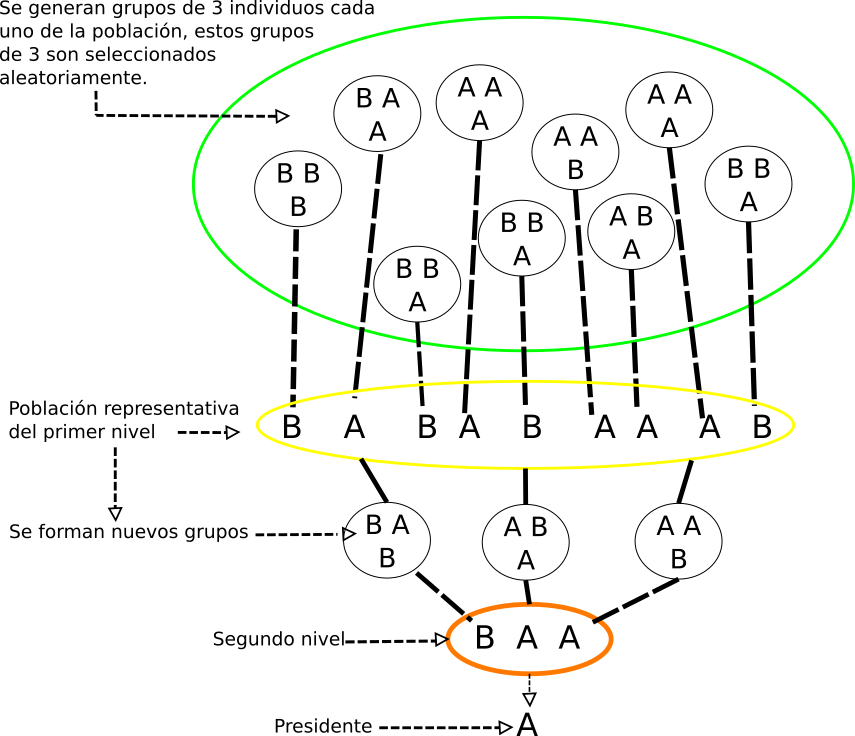
\includegraphics[scale=0.50]{TT/img/marco teorico/prediccion.png}
    \caption{Jerarquización de la población a través de diferentes iteraciones}
    \label{graphic:prediccion}
\end{figure}

Por lo tanto, la votación por regla de la mayoría produce la auto-eliminación de cualquier proporción de la tendencia \textbf{A}, mientras que $p_{0} < 1/2$, siempre que exista un número suficiente de votación, esto lo vemos en la figura \ref{graphic:prediccion}. Por consiguiente, es esencial determinar el número de niveles necesarios para garantizar el liderazgo completo a la mayor tendencia inicial. \cite{Galam2008}
%Insertar imagen describiendo el funcionamiento del algoritmo

\subsection{Grupos de votación mas grandes y la fórmula mágica}
Para grupos de votación de cualquier tamaño \textbf{\textit{r}} la función de votación $p_{n+1} = P_{r}(p_{n})$ se escribe:
\begin{equation}
    P_{r}(p_{n}) = \sum_{l=r}^{l=m} \frac{r!}{l!(r-l)!}p_{n}^{l}(1+p_{n})^{r-l},
\end{equation}
donde $m = (r + 1)/2$ para r impar y $m = (r + 1)/2$ para r par para dar cuenta del sesgo favorecido por \textbf{B}. Los dos puntos fijos estables $p_{d} = 0$ y $p_{t} = 1$ son independientes del tamaño del grupo \textbf{\textit{r}}. La inestable $p_{c,r} = 1/2$ también es independiente del tamaño del grupo \textbf{\textit{r}} para valores impares de r, para los cuales no existe sesgo. Por el contrario, varía con \textbf{\textit{r}} para valores pares. Comienza en $p_{c,2} = 1$ para $r = 2$, disminuye a $p_{c,4} = (1 + \sqrt{13})/6 \approx 0.77$ para $\textbf{\textit{r}} = 4$ y luego sigue disminuyendo asintóticamente hacia $1/2$ desde arriba.


\chapter{Análisis} \label{analisis}
\epigraph{\textit{Research is what I'm doing when I don't know what I'm doing.   
	}}{\textit{— Wernher von Braun, NASA engineer}}
	\vspace*{8cm}
	\begin{center}
		\centering
		\includegraphics[width=10.5cm]{example-image}
    \end{center}
\thispagestyle{empty}
\newpage
\vspace*{2cm}

\section{Estudio de factibilidad}
En esta sección del trabajo terminal, abordaremos la factibilidad técnica y económica que tendrá la implementación de la solución propuesta. Para ello se dará respuesta a las siguientes preguntas sobre la factibilidad del sistema.

\textbf{\textit{¿Este sistema implementará alguna tecnología que no se haya empleado previamente?}}\newline
Para el desarrollo del sistema no requerirá alguna tecnología que no se haya implementado anteriormente, ya que los usuarios deberán contar con un dispositivo móvil para realizar las actividades necesarias para el funcionamiento de este. 

\textbf{\textit{¿El sistema puede integrarse dentro de alguna organización?}}\newline
El sistema se plantea como un sistema independiente, pero, puede hacerlo adaptando el sistema para que sea consumido por otros que estén en la organización que lo use.

\textbf{\textit{Considerando gastos, tecnología, conocimiento y tiempo ¿El desarrollo del sistema es conveniente?}}\newline
La respuesta es sí, ya que la tecnología que implementará tiene una gran comunidad y tiene años en el mercado, lo único necesario es acceso a un equipo de computo y tener acceso a internet, con lo que ya se cuenta. Los problemas son la falta de conocimiento técnico con algunos temas, sin embargo, el tiempo y apoyándose con la comunidad de desarrolladores que tiene las tecnologías a usar, se puede superar este problema, por otro lado puede que algunas tecnologías tengan algún costo, pero como se tiene acceso a una cuenta universitaria, existen descuentos o inclusive el uso gratuito de la tecnología que se requiera.

Por lo tanto, podemos concluir que el sistema es factible de manera técnica y económicamente.
\subsection{Herramientas necesarias para el desarrollo del sistema}

\subsection{Elección de software}

\section{Metodología}
Para este trabajo terminal se utilizará la metodología de desarrollo rápido de aplicaciones (DRA), dado que el tiempo de desarrollo es corto, esta metodología permite centrarse en el producto final, hace hincapié en el desarrollo de prioridades y la definición de los plazos de entrega, si estos empiezan a atrasarse permite la reducción de requisitos para el ajuste y de esta manera no aumentar la fecha limite de entrega. Por otro lado la participación de los usuarios es necesaria para el diseño del sistema.\cite{dra}

\begin{figure}[!ht]
    \centering
    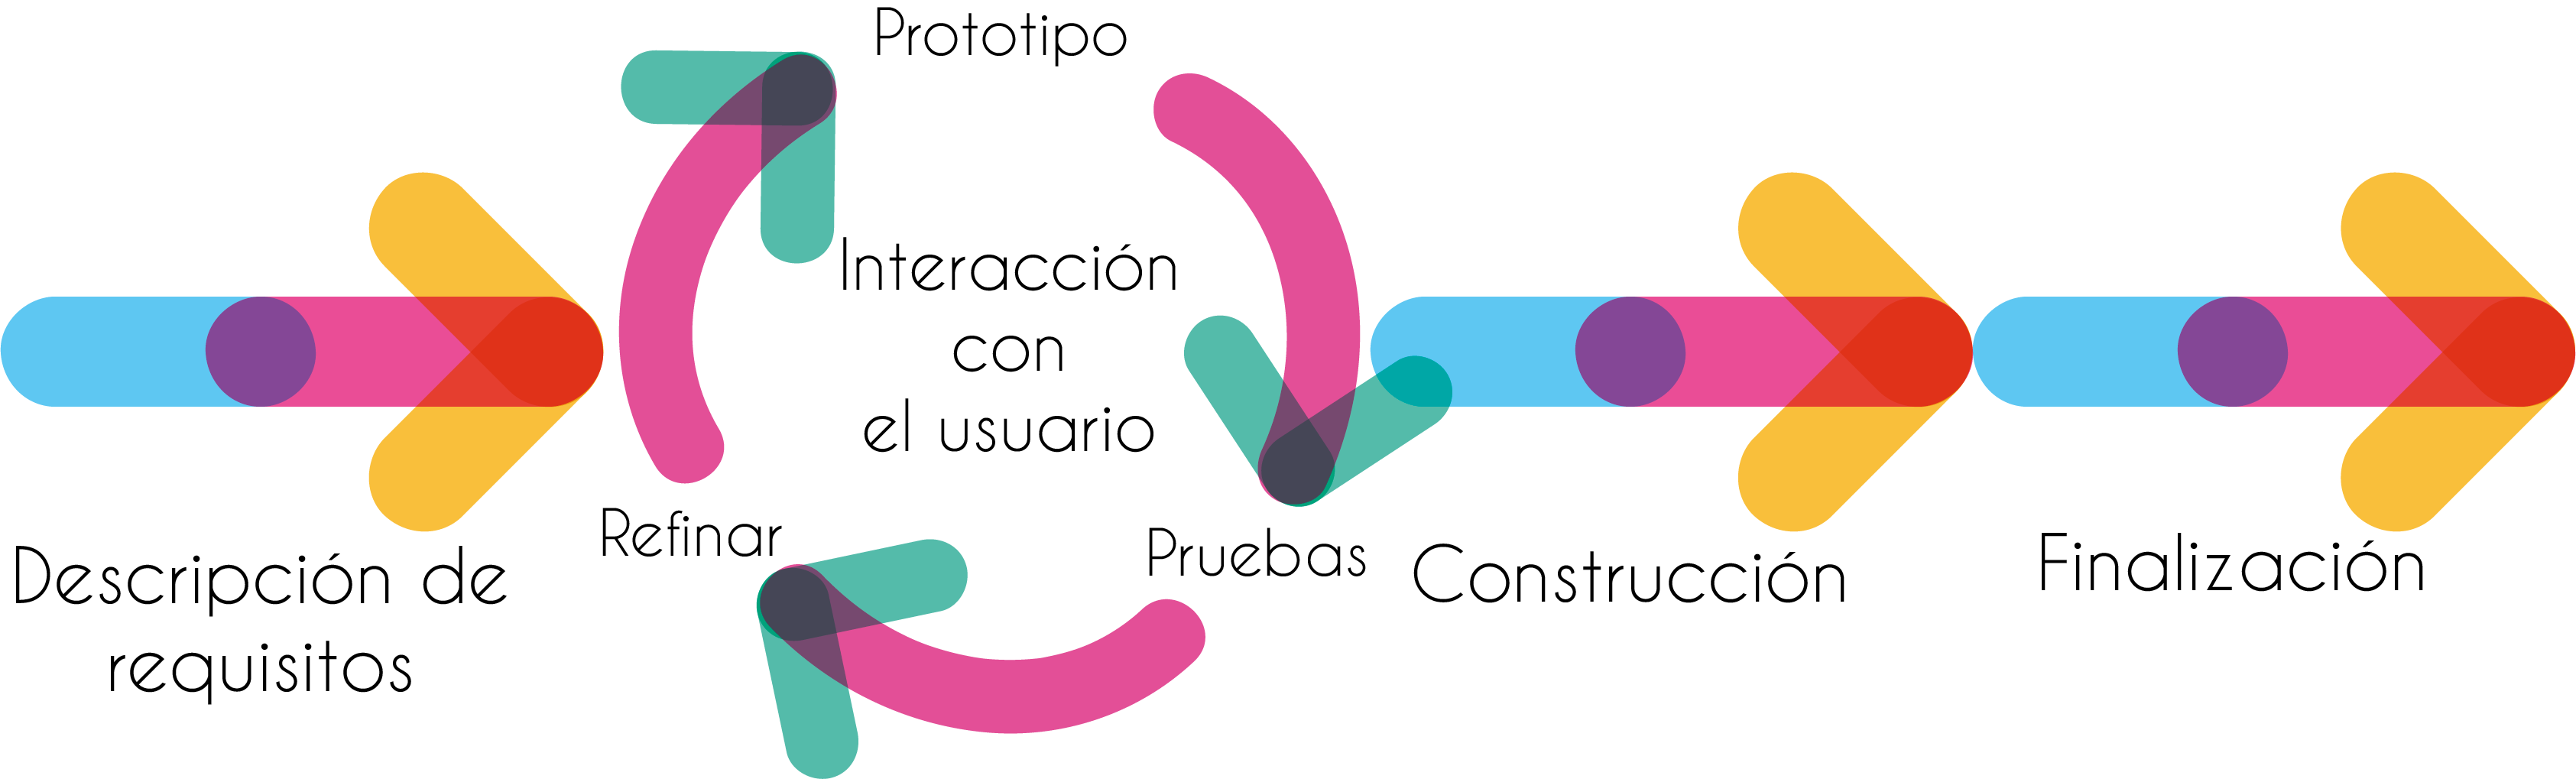
\includegraphics[scale=0.50]{TT/img/metodología/RAD.png}
    \caption{Desarrollo rápido de aplicaciones}
    \label{graphic:RAD}
\end{figure}
\section{Requerimientos}

\subsection{Requerimientos funcionales}

\subsection{Requerimientos no funcionales}


\chapter{Diseño}\label{diseno}

%\epigraph{\textit{Sometimes it is the people no one imagines anything of who do the things that no one can imagine.  
%}}{\textit{— Alan Turing}}
%\vspace*{8cm}
%\begin{center}
%	\centering
%	\includegraphics[width=10.5cm]{example-image}
%\end{center}
%\thispagestyle{empty}
%\newpage
\vspace*{2cm}

En el siguiente capítulo se ve detalla más a fondo de las reglas de negocio que debe cumplir el sistema, así mismo, el modelo relacional, la arquitectura del sistema usando UML.

\section{Reglas de negocio}
\begin{longtable}{|l|m{4cm}|m{9.5cm}|}
    \hline
    \rowcolor[HTML]{329A9D} 
    \multicolumn{3}{|c|}{\cellcolor[HTML]{329A9D}{\color[HTML]{FFFFFF} Reglas de negocio}} \\ \hline
    \rowcolor[HTML]{3531FF} 
    \multicolumn{1}{|c|}{\cellcolor[HTML]{3531FF}{\color[HTML]{FFFFFF} ID}} & \multicolumn{1}{c|}{\cellcolor[HTML]{3531FF}{\color[HTML]{FFFFFF} Nombre}} & \multicolumn{1}{c|}{\cellcolor[HTML]{3531FF}{\color[HTML]{FFFFFF} Descripción}} \\ \hline
    \endfirsthead
    \hline
    \rowcolor[HTML]{329A9D} 
    \multicolumn{3}{|c|}{\cellcolor[HTML]{329A9D}{\color[HTML]{FFFFFF} Reglas de negocio}} \\ \hline
    \rowcolor[HTML]{3531FF} 
    \multicolumn{1}{|c|}{\cellcolor[HTML]{3531FF}{\color[HTML]{FFFFFF} ID}} & \multicolumn{1}{c|}{\cellcolor[HTML]{3531FF}{\color[HTML]{FFFFFF} Nombre}} & \multicolumn{1}{c|}{\cellcolor[HTML]{3531FF}{\color[HTML]{FFFFFF} Descripción}} \\ \hline
    \endhead
    % aquí añadimos el fondo de todas las hojas, excepto de la última.
    \multicolumn{3}{c}{Sigue en la página siguiente.}
    \endfoot
    % aquí añadimos el fondo de la última hoja.
    \endlastfoot
    RN01&Encuestas&Las encuestas serán limitadas a preguntas de opción múltiple. \\ \hline
    RN02&Peso de respuestas & El peso por defecto a cada respuesta creada será de 1.\\ \hline
    RN03&Datos obligatorios & Los datos que serán necesarios para registrarse son: Nombre y apellidos, correo electrónico, sexo y su contraseña.\\ \hline
    RN04&Usuarios identificados & Los usuarios tendrán que iniciar sesión para contestar y crear encuestas.\\ \hline
    RN05&Identificador de usuario único & La dirección de correo electrónico registrada será el identificador de cada usuario, por lo que no podrá haber duplicados.\\ \hline
    \caption{Reglas de negocio}
    \label{table:RNegocio}
\end{longtable}
\section{Casos de uso}
Los requerimientos del sistema se transforman en casos de uso necesarios para plantear la infraestructura del sistema a nivel de implementación, el diagrama de casos de uso se muestra a continuación.

\subsection{Gestionar encuesta}

\begin{figure}[!ht]
    \centering
    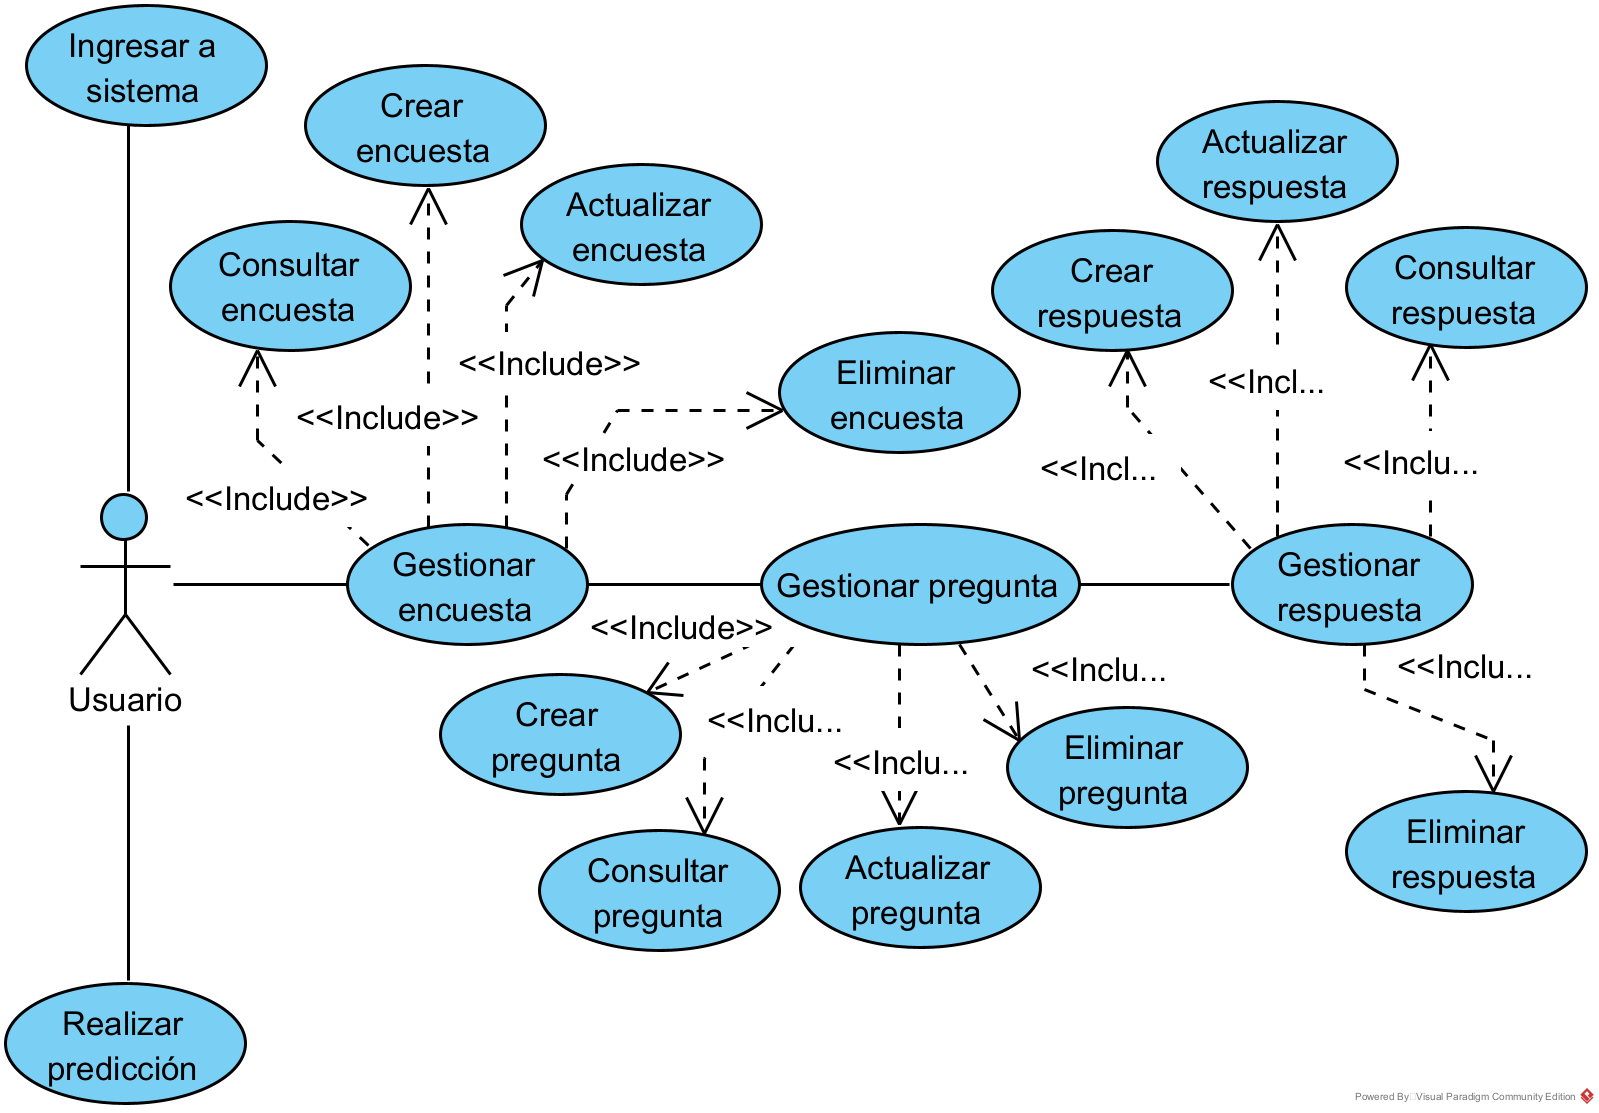
\includegraphics[scale=1.0]{TT/img/diseño/Crear encuesta.png}
    \caption{Diagrama de caso de uso sobre la gestión de encuestas }
    \label{graphic:CU-D-gestionar-encuesta}
\end{figure}


\subsection{Contestar encuesta}

\begin{figure}[!ht]
    \centering
    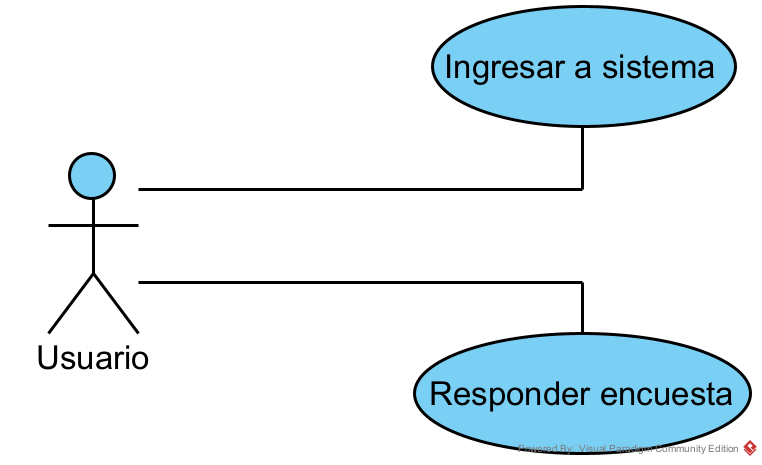
\includegraphics[scale=1.0]{TT/img/diseño/Responder encuesta.png}
    \caption{Diagrama de caso de uso sobre contestar encuesta}
    \label{graphic:CU-D-contestar-encuesta}
\end{figure}


\section{Especificación de casos de uso}

En esta sección se describen detalladamente todos los casos de uso del sistema.

\subsection{Ingresar al sistema}

\begin{longtable}{|>{\columncolor[HTML]{3531FF}}m{3cm}|m{11cm}|}
    \hline
    {\color[HTML]{FFFFFF} Caso de uso} & Ingresar sistema \\ \hline
    \endfirsthead
    \hline
    {\color[HTML]{FFFFFF} Caso de uso} & Ingresar sistema \\
    \hline 
    \endhead
    % aquí añadimos el fondo de todas las hojas, excepto de la última.
    \multicolumn{2}{c}{Sigue en la página siguiente.}
    \endfoot
    % aquí añadimos el fondo de la última hoja.
    \endlastfoot
    \hline
    {\color[HTML]{FFFFFF} Actores}& Usuario\\ \hline
    {\color[HTML]{FFFFFF} Resumen}& El usuario ingresa al sistema y se identifica\\ \hline
    {\color[HTML]{FFFFFF} Precondiciones}& Ninguna \\ \hline
    {\color[HTML]{FFFFFF} Flujo principal}& \begin{enumerate}
            \item El usuario se identifica mediante correo y contraseña e ingresa al modulo principal del sistema.
            \item Búsqueda de usuario existente.
            \item El sistema verifica que el usuario exista, el caso de uso termina.
        \end{enumerate}\\ \hline
    {\color[HTML]{FFFFFF} Subflujos}& \begin{enumerate}
        \item El usuario se identifica mediante correo y contraseña e ingresa al modulo principal del sistema.
    \end{enumerate}\\ \hline
    {\color[HTML]{FFFFFF} Excepciones}& \textbf{Usuario invalido:} El sistema informa que su usuario o contraseña no es correcto, el caso de uso termina.\\ \hline
    {\color[HTML]{FFFFFF} Postcondiciones}& \textbf{Usuario en sección correcta:} El usuario se encontrará en la parte del sistema que le corresponde.\\ \hline
    {\color[HTML]{FFFFFF} Escenarios de éxito}& \textbf{Un usuario ingresa al sistema:} El usuario ingresa correctamente al sistema.\\ \hline
    {\color[HTML]{FFFFFF} Escenarios de fracaso}& \textbf{Usuario identificado incorrectamente:} Usuario o contraseña inválido.\\ \hline
    \caption{Especificación de caso de uso de ingresar al sistema}
    \label{table:CU01}
\end{longtable}

\subsection{Crear encuesta}

\begin{longtable}{|>{\columncolor[HTML]{3531FF}}m{3cm}|m{11cm}|}
    \hline
    {\color[HTML]{FFFFFF} Caso de uso} & Crear encuesta\\ \hline
    \endfirsthead
    \hline
    {\color[HTML]{FFFFFF} Caso de uso} & Crear encuesta \\
    \hline 
    \endhead
    % aquí añadimos el fondo de todas las hojas, excepto de la última.
    \multicolumn{2}{c}{Sigue en la página siguiente.}
    \endfoot
    % aquí añadimos el fondo de la última hoja.
    \endlastfoot
    \hline
    {\color[HTML]{FFFFFF} Actores}& Usuario\\ \hline
    {\color[HTML]{FFFFFF} Resumen}& El usuario crea una encuesta que será almacenada en la base de datos.\\ \hline
    {\color[HTML]{FFFFFF} Precondiciones}& \textbf{Usuario identificado: }Usuario correctamente identificado \\ \hline
    {\color[HTML]{FFFFFF} Flujo principal}& \begin{enumerate}
            \item El usuario se dirige a la sección de encuestas.
            \item El usuario elige la opción de crear encuesta.
            \item El sistema muestra la pantalla para crear encuesta.
            \item El usuario ingresa los datos para crear encuesta.
            \item El usuario guarda la encuesta.
            \item El sistema guarda la encuesta en la base de datos, el caso de uso termina.
        \end{enumerate}\\ \hline
    {\color[HTML]{FFFFFF} Subflujos}& \textbf{Guardar encuesta}
    \begin{enumerate}
        \item El sistema verificará que todos los campos obligatorios se hayan llenado.
        \item El sistema guardará la encuesta en la base de datos.
    \end{enumerate}\\ \hline
    {\color[HTML]{FFFFFF} Excepciones}& \textbf{Guardar encuesta: }El sistema informará cuando la encuesta no se haya guardado correctamente.\\ \hline
    {\color[HTML]{FFFFFF} Postcondiciones}& \textbf{Encuesta almacenada: } La encuesta se almacena correctamente en la base de datos.\\ \hline
    {\color[HTML]{FFFFFF} Escenarios de éxito}& \textbf{La encuesta se almacena: }La encuesta se almacena exitosamente en la base de datos.\\ \hline
    {\color[HTML]{FFFFFF} Escenarios de fracaso}& \textbf{La encuesta no se almacena: }La encuesta no se almacena en la base de datos.\\ \hline
    \caption{Especificación de caso de uso de crear encuesta}
    \label{table:CU02}
\end{longtable}

\subsection{Consultar encuesta}

\begin{longtable}{|>{\columncolor[HTML]{3531FF}}m{3cm}|m{11cm}|}
    \hline
    {\color[HTML]{FFFFFF} Caso de uso} & Consultar encuesta \\ \hline
    \endfirsthead
    \hline
    {\color[HTML]{FFFFFF} Caso de uso} & Consultar encuesta \\
    \hline 
    \endhead
    % aquí añadimos el fondo de todas las hojas, excepto de la última.
    \multicolumn{2}{c}{Sigue en la página siguiente.}
    \endfoot
    % aquí añadimos el fondo de la última hoja.
    \endlastfoot
    \hline
    {\color[HTML]{FFFFFF} Actores}& Usuario\\ \hline
    {\color[HTML]{FFFFFF} Resumen}& El usuario consulta las encuestas creadas por el mismo.\\ \hline
    {\color[HTML]{FFFFFF} Precondiciones}& Usuario esta correctamente identificado \\ \hline
    {\color[HTML]{FFFFFF} Flujo principal}& \begin{enumerate}
            \item El usuario se dirige a la sección de encuestas.
            \item En la sección de encuestas, selecciona la opción de ver sus encuestas.
            \item El sistema muestra las encuestas creadas por el usuario.
        \end{enumerate}\\ \hline
    {\color[HTML]{FFFFFF} Subflujos}& Ninguno. \\ \hline
    {\color[HTML]{FFFFFF} Excepciones}& \textbf{Lista vacía: }No existen encuestas guardadas anteriormente.\\ \hline
    {\color[HTML]{FFFFFF} Postcondiciones}& \textbf{Encuestas mostradas:} Las encuestas correspondientes son mostradas correctamente.\\ \hline
    {\color[HTML]{FFFFFF} Escenarios de éxito}& \textbf{Las encuestas se muestran: } Las encuestas son mostradas al usuario.\\ \hline
    {\color[HTML]{FFFFFF} Escenarios de fracaso}& \textbf{Lista vacía:} Lista de encuestas vacías.\\ \hline
    \caption{Especificación de caso de uso de consultar encuesta}
    \label{table:CU04}
\end{longtable}

\subsection{Editar encuesta}

\begin{longtable}{|>{\columncolor[HTML]{3531FF}}m{3cm}|m{11cm}|}
    \hline
    {\color[HTML]{FFFFFF} Caso de uso} & Editar encuesta \\ \hline
    \endfirsthead
    \hline
    {\color[HTML]{FFFFFF} Caso de uso} & Editar encuesta \\
    \hline 
    \endhead
    % aquí añadimos el fondo de todas las hojas, excepto de la última.
    \multicolumn{2}{c}{Sigue en la página siguiente.}
    \endfoot
    % aquí añadimos el fondo de la última hoja.
    \endlastfoot
    \hline
    {\color[HTML]{FFFFFF} Actores}& Usuario\\ \hline
    {\color[HTML]{FFFFFF} Resumen}& El usuario modifica una encuesta existente creada por el mismo.\\ \hline
    {\color[HTML]{FFFFFF} Precondiciones}& El usuario esta correctamente identificado. \\ \hline
    {\color[HTML]{FFFFFF} Flujo principal}& \begin{enumerate}
            \item El usuario se dirige a la sección de encuestas.
            \item En la sección de encuestas, selecciona la opción de ver sus encuestas.
            \item El usuario selecciona una encuesta suya que va a modificar.
            \item Elige la opción de editar encuesta.
            \item El usuario modifica la encuesta seleccionada.
            \item El usuario guarda los cambios realizados en su encuesta, el caso de uso termina.
        \end{enumerate}\\ \hline
    {\color[HTML]{FFFFFF} Subflujos}& Ninguno. \\ \hline
    {\color[HTML]{FFFFFF} Excepciones}& \textbf{Lista vacía: }No existen encuestas guardadas anteriormente.\\ \hline
    {\color[HTML]{FFFFFF} Postcondiciones}& \textbf{Encuesta modificada: }La encuesta se ha modificado correctamente..\\ \hline
    {\color[HTML]{FFFFFF} Escenarios de éxito}& \textbf{La encuesta se modifica:} La encuesta se modifica correctamente.\\ \hline
    {\color[HTML]{FFFFFF} Escenarios de fracaso}& \textbf{La encuesta no se modifica:} La encuesta no se modifica correctamente.\\ \hline
    \caption{Especificación de caso de uso de editar encuesta}
    \label{table:CU03}
\end{longtable}

\subsection{Eliminar encuesta}

\begin{longtable}{|>{\columncolor[HTML]{3531FF}}m{3cm}|m{11cm}|}
    \hline
    {\color[HTML]{FFFFFF} Caso de uso} & Eliminar encuesta \\ \hline
    \endfirsthead
    \hline
    {\color[HTML]{FFFFFF} Caso de uso} & Eliminar encuesta \\
    \hline 
    \endhead
    % aquí añadimos el fondo de todas las hojas, excepto de la última.
    \multicolumn{2}{c}{Sigue en la página siguiente.}
    \endfoot
    % aquí añadimos el fondo de la última hoja.
    \endlastfoot
    \hline
    {\color[HTML]{FFFFFF} Actores}& Usuario\\ \hline
    {\color[HTML]{FFFFFF} Resumen}& El usuario elimina una encuesta\\ \hline
    {\color[HTML]{FFFFFF} Precondiciones}& Usuario esta correctamente identificado \\ \hline
    {\color[HTML]{FFFFFF} Flujo principal}& \begin{enumerate}
            \item El usuario se dirige a la sección de encuestas.
            \item En la sección de encuestas, selecciona la opción de ver sus encuestas.
            \item El sistema muestra las encuestas creadas por el usuario.
            \item El usuario selecciona la encuesta a eliminar.
            \item El usuario selecciona la opción de eliminar encuesta.
            \item El sistema le solicita la verificación de eliminación al usuario.
            \item El usuario acepta eliminar la encuesta.
            \item El sistema elimina la encuesta, el caso de uso termina.
        \end{enumerate}\\ \hline
    {\color[HTML]{FFFFFF} Subflujos}& Ninguno.\\ \hline
    {\color[HTML]{FFFFFF} Excepciones}& \textbf{Cancelación de la eliminación: }El usuario cancela la eliminación de la encuesta.\\ \hline
    {\color[HTML]{FFFFFF} Postcondiciones}& \textbf{Encuesta eliminada: }La encuesta es eliminada de la base de datos.\\ \hline
    {\color[HTML]{FFFFFF} Escenarios de éxito}& \textbf{La encuesta se elimina: }La pregunta se elimina correctamente de la base de datos.\\ \hline
    {\color[HTML]{FFFFFF} Escenarios de fracaso}& \textbf{La encuesta no se elimina: }La encuesta no se elimina de la base de datos.\\ \hline
    \caption{Especificación de caso de uso de eliminar encuesta}
    \label{table:CU05}
\end{longtable}

\subsection{Crear pregunta}

\begin{longtable}{|>{\columncolor[HTML]{3531FF}}m{3cm}|m{11cm}|}
    \hline
    {\color[HTML]{FFFFFF} Caso de uso} & Crear pregunta \\ \hline
    \endfirsthead
    \hline
    {\color[HTML]{FFFFFF} Caso de uso} & Crear pregunta \\
    \hline 
    \endhead
    % aquí añadimos el fondo de todas las hojas, excepto de la última.
    \multicolumn{2}{c}{Sigue en la página siguiente.}
    \endfoot
    % aquí añadimos el fondo de la última hoja.
    \endlastfoot
    \hline
    {\color[HTML]{FFFFFF} Actores}& Usuario\\ \hline
    {\color[HTML]{FFFFFF} Resumen}& El usuario crea una pregunta que será almacenada en la base de datos.\\ \hline
    {\color[HTML]{FFFFFF} Precondiciones}& \textbf{Usuario identificado: }Usuario correctamente identificado  y tiene que tener al menos una encuesta creada.\\ \hline
    {\color[HTML]{FFFFFF} Flujo principal}& \begin{enumerate}
            \item El usuario se dirige a la sección de encuestas.
            \item El usuario elige la opción de ver sus encuestas.
            \item El usuario elige la encuesta deseada para agregar preguntas.
            \item El sistema muestra la información de la encuesta.
            \item El usuario selección agregar pregunta.
            \item El usuario ingresa los datos para crear pregunta.
            \item El usuario guarda la pregunta.
            \item El sistema guarda la pregunta en la base de datos, el caso de uso termina.
        \end{enumerate}\\ \hline
    {\color[HTML]{FFFFFF} Subflujos}& \textbf{Guardar pregunta}
    \begin{enumerate}
        \item El sistema verificará que todos los campos obligatorios se hayan llenado.
        \item El sistema guardará la pregunta en la base de datos.
    \end{enumerate}\\ \hline
    {\color[HTML]{FFFFFF} Excepciones}& \textbf{Guardar pregunta: }El sistema informará cuando la pregunta no se haya guardado correctamente.\\ \hline
    {\color[HTML]{FFFFFF} Postcondiciones}& \textbf{Pregunta almacenada: } La pregunta se almacena correctamente en la base de datos.\\ \hline
    {\color[HTML]{FFFFFF} Escenarios de éxito}& \textbf{La pregunta se almacena: }La pregunta se almacena exitosamente en la base de datos.\\ \hline
    {\color[HTML]{FFFFFF} Escenarios de fracaso}& \textbf{La pregunta no se almacena: }La pregunta no se almacena en la base de datos.\\ \hline
    \caption{Especificación de caso de uso de crear pregunta}
    \label{table:CU06}
\end{longtable}

\subsection{Consultar pregunta}

\begin{longtable}{|>{\columncolor[HTML]{3531FF}}m{3cm}|m{11cm}|}
    \hline
    {\color[HTML]{FFFFFF} Caso de uso} & Consultar pregunta \\ \hline
    \endfirsthead
    \hline
    {\color[HTML]{FFFFFF} Caso de uso} & Consultar pregunta \\
    \hline 
    \endhead
    % aquí añadimos el fondo de todas las hojas, excepto de la última.
    \multicolumn{2}{c}{Sigue en la página siguiente.}
    \endfoot
    % aquí añadimos el fondo de la última hoja.
    \endlastfoot
    \hline
    {\color[HTML]{FFFFFF} Actores}& Usuario\\ \hline
     {\color[HTML]{FFFFFF} Resumen}& El usuario consulta las preguntas creadas por el mismo.\\ \hline
    {\color[HTML]{FFFFFF} Precondiciones}& Usuario esta correctamente identificado y tiene que tener al menos una encuesta creada.\\ \hline
    {\color[HTML]{FFFFFF} Flujo principal}& \begin{enumerate}
            \item El usuario se dirige a la sección de encuestas.
            \item El usuario elige la opción de ver sus encuestas.
            \item El usuario elige la encuesta deseada.
            \item El sistema muestra la información de la encuesta junto con sus preguntas.
        \end{enumerate}\\ \hline
    {\color[HTML]{FFFFFF} Subflujos}& Ninguno. \\ \hline
    {\color[HTML]{FFFFFF} Excepciones}& \textbf{Lista vacía: }No existen preguntas guardadas anteriormente.\\ \hline
    {\color[HTML]{FFFFFF} Postcondiciones}& \textbf{Preguntas mostradas:} Las preguntas correspondientes son mostradas correctamente.\\ \hline
    {\color[HTML]{FFFFFF} Escenarios de éxito}& \textbf{Las preguntas se muestran: } Las preguntas son mostradas al usuario.\\ \hline
    {\color[HTML]{FFFFFF} Escenarios de fracaso}& \textbf{Lista vacía:} Lista de preguntas vacías.\\ \hline
    \caption{Especificación de caso de uso de consultar pregunta}
    \label{table:CU08}
\end{longtable}

\subsection{Editar pregunta}

\begin{longtable}{|>{\columncolor[HTML]{3531FF}}m{3cm}|m{11cm}|}
    \hline
    {\color[HTML]{FFFFFF} Caso de uso} & Editar pregunta \\ \hline
    \endfirsthead
    \hline
    {\color[HTML]{FFFFFF} Caso de uso} & Editar pregunta \\
    \hline 
    \endhead
    % aquí añadimos el fondo de todas las hojas, excepto de la última.
    \multicolumn{2}{c}{Sigue en la página siguiente.}
    \endfoot
    % aquí añadimos el fondo de la última hoja.
    \endlastfoot
    \hline
    {\color[HTML]{FFFFFF} Actores}& Usuario\\ \hline
    {\color[HTML]{FFFFFF} Resumen}& El usuario modifica una pregunta existente de una encuesta creada por el mismo.\\ \hline
    {\color[HTML]{FFFFFF} Precondiciones}& El usuario esta correctamente identificado  y tiene que tener al menos una encuesta creada. \\ \hline
    {\color[HTML]{FFFFFF} Flujo principal}& \begin{enumerate}
            \item El usuario se dirige a la sección de encuestas.
            \item El usuario elige la opción de ver sus encuestas.
            \item El usuario elige la encuesta deseada.
            \item El sistema muestra la información de la encuesta junto con sus preguntas.
            \item El sistema muestra la información de la encuesta.
            \item El usuario selecciona una pregunta suya que va a modificar.
            \item Elige la opción de editar pregunta.
            \item El usuario modifica la pregunta seleccionada.
            \item El usuario guarda los cambios realizados en su pregunta, el caso de uso termina.
        \end{enumerate}\\ \hline
    {\color[HTML]{FFFFFF} Subflujos}& Ninguno. \\ \hline
    {\color[HTML]{FFFFFF} Excepciones}& \textbf{Lista vacía: }No existen preguntas guardadas anteriormente.\\ \hline
    {\color[HTML]{FFFFFF} Postcondiciones}& \textbf{Pregunta modificada: }La pregunta se ha modificado correctamente.\\ \hline
    {\color[HTML]{FFFFFF} Escenarios de éxito}& \textbf{La pregunta se modifica:} La pregunta se modifica correctamente.\\ \hline
    {\color[HTML]{FFFFFF} Escenarios de fracaso}& \textbf{La pregunta no se modifica:} La pregunta no se modifica correctamente.\\ \hline
    \caption{Especificación de caso de uso de editar pregunta}
    \label{table:CU07}
\end{longtable}

\subsection{Eliminar pregunta}

\begin{longtable}{|>{\columncolor[HTML]{3531FF}}m{3cm}|m{11cm}|}
    \hline
    {\color[HTML]{FFFFFF} Caso de uso} & Eliminar pregunta \\ \hline
    \endfirsthead
    \hline
    {\color[HTML]{FFFFFF} Caso de uso} & Eliminar pregunta \\
    \hline 
    \endhead
    % aquí añadimos el fondo de todas las hojas, excepto de la última.
    \multicolumn{2}{c}{Sigue en la página siguiente.}
    \endfoot
    % aquí añadimos el fondo de la última hoja.
    \endlastfoot
    \hline
    {\color[HTML]{FFFFFF} Actores}& Usuario\\ \hline
    {\color[HTML]{FFFFFF} Resumen}& El usuario elimina una pregunta de una encuesta creada por el mismo\\ \hline
    {\color[HTML]{FFFFFF} Precondiciones}& Usuario esta correctamente identificado  y tiene que tener al menos una encuesta creada.\\ \hline
    {\color[HTML]{FFFFFF} Flujo principal}& \begin{enumerate}
            \item El usuario se dirige a la sección de encuestas.
            \item El usuario elige la opción de ver sus encuestas.
            \item El usuario elige la encuesta deseada.
            \item El sistema muestra la información de la encuesta junto con sus preguntas.
            \item El sistema muestra la información de la encuesta junto con sus preguntas.
            \item El usuario selecciona una pregunta suya que va a eliminar.
            \item Elige la opción de eliminar pregunta.
            \item El usuario elimina la pregunta seleccionada.
            \item El sistema le notifica al usuario sobre la eliminación de la pregunta.
            \item El usuario confirma la eliminación de su pregunta.
            \item El sistema elimina la pregunta de la base de datos.
        \end{enumerate}\\ \hline
    {\color[HTML]{FFFFFF} Subflujos}& Ninguno.\\ \hline
    {\color[HTML]{FFFFFF} Excepciones}& \textbf{Cancelación de la eliminación: }El usuario cancela la eliminación de la pregunta.\\ \hline
    {\color[HTML]{FFFFFF} Postcondiciones}& \textbf{Pregunta eliminada: }La pregunta es eliminada de la base de datos.\\ \hline
    {\color[HTML]{FFFFFF} Escenarios de éxito}& \textbf{La Pregunta se elimina: }La pregunta se elimina correctamente de la base de datos.\\ \hline
    {\color[HTML]{FFFFFF} Escenarios de fracaso}& \textbf{La pregunta no se elimina: }La pregunta no se elimina de la base de datos.\\ \hline
    \caption{Especificación de caso de uso de Eliminar pregunta}
    \label{table:CU09}
\end{longtable}

\subsection{Crear respuesta}

\begin{longtable}{|>{\columncolor[HTML]{3531FF}}m{3cm}|m{11cm}|}
    \hline
    {\color[HTML]{FFFFFF} Caso de uso} & Crear respuesta \\ \hline
    \endfirsthead
    \hline
    {\color[HTML]{FFFFFF} Caso de uso} & Crear respuesta \\
    \hline 
    \endhead
    % aquí añadimos el fondo de todas las hojas, excepto de la última.
    \multicolumn{2}{c}{Sigue en la página siguiente.}
    \endfoot
    % aquí añadimos el fondo de la última hoja.
    \endlastfoot
    \hline
    {\color[HTML]{FFFFFF} Actores}& Usuario\\ \hline
    {\color[HTML]{FFFFFF} Resumen}& El usuario crea una respuesta para una pregunta de una encuesta que será almacenada en la base de datos.\\ \hline
    {\color[HTML]{FFFFFF} Precondiciones}& \textbf{Usuario identificado: }Usuario correctamente identificado  y tiene que tener al menos una encuesta creada con al menos una pregunta creada.\\ \hline
    {\color[HTML]{FFFFFF} Flujo principal}& \begin{enumerate}
            \item El usuario se dirige a la sección de encuestas.
            \item El usuario elige la opción de ver sus encuestas.
            \item El usuario elige la encuesta deseada para agregar preguntas.
            \item El sistema muestra la información de la encuesta.
            \item El usuario selecciona una pregunta.
            \item El usuario selecciona agregar una opción.
            \item El usuario ingresa los datos para crear una opción de respuesta.
            \item El usuario guarda la opción de respuesta.
            \item El sistema guarda la opción de respuesta en la base de datos, el caso de uso termina.
        \end{enumerate}\\ \hline
    {\color[HTML]{FFFFFF} Subflujos}& \textbf{Guardar opción de respuesta}
    \begin{enumerate}
        \item El sistema verificará que todos los campos obligatorios se hayan llenado.
        \item El sistema guardará la pregunta en la base de datos.
    \end{enumerate}\\ \hline
    {\color[HTML]{FFFFFF} Excepciones}& \textbf{Guardar pregunta: }El sistema informará cuando la pregunta no se haya guardado correctamente.
    \\ \hline
    {\color[HTML]{FFFFFF} Postcondiciones}& \textbf{Opción de respuesta almacenada: } La opción se almacena correctamente en la base de datos.\\ \hline
    {\color[HTML]{FFFFFF} Escenarios de éxito}& \textbf{La opción se almacena: }La opción se almacena exitosamente en la base de datos.\\ \hline
    {\color[HTML]{FFFFFF} Escenarios de fracaso}& \textbf{La opción no se almacena: }La opción no se almacena en la base de datos.\\ \hline
    \caption{Especificación de caso de uso de crear respuesta}
    \label{table:CU10}
\end{longtable}

\subsection{Consultar respuesta}

\begin{longtable}{|>{\columncolor[HTML]{3531FF}}m{3cm}|m{11cm}|}
    \hline
    {\color[HTML]{FFFFFF} Caso de uso} & Consultar respuesta \\ \hline
    \endfirsthead
    \hline
    {\color[HTML]{FFFFFF} Caso de uso} & Consultar respuesta \\
    \hline 
    \endhead
    % aquí añadimos el fondo de todas las hojas, excepto de la última.
    \multicolumn{2}{c}{Sigue en la página siguiente.}
    \endfoot
    % aquí añadimos el fondo de la última hoja.
    \endlastfoot
    \hline
    {\color[HTML]{FFFFFF} Actores}& Usuario\\ \hline
     {\color[HTML]{FFFFFF} Resumen}& El usuario consulta las preguntas creadas por el mismo.\\ \hline
    {\color[HTML]{FFFFFF} Precondiciones}& Usuario esta correctamente identificado y tiene que tener al menos una encuesta creada.\\ \hline
    {\color[HTML]{FFFFFF} Flujo principal}& \begin{enumerate}
            \item El usuario se dirige a la sección de encuestas.
            \item El usuario elige la opción de ver sus encuestas.
            \item El usuario elige la encuesta deseada.
            \item El sistema muestra la información de la encuesta junto con sus preguntas.
            \item El usuario visualiza todas las preguntas con sus opciones de respuesta de la encuesta seleccionada.
        \end{enumerate}\\ \hline
    {\color[HTML]{FFFFFF} Subflujos}& Ninguno. \\ \hline
    {\color[HTML]{FFFFFF} Excepciones}& \textbf{Lista vacía: }No existen preguntas guardadas anteriormente.\\ \hline
    {\color[HTML]{FFFFFF} Postcondiciones}& \textbf{Preguntas mostradas:} Las preguntas correspondientes son mostradas correctamente.\\ \hline
    {\color[HTML]{FFFFFF} Escenarios de éxito}& \textbf{Las preguntas se muestran: } Las preguntas son mostradas al usuario.\\ \hline
    {\color[HTML]{FFFFFF} Escenarios de fracaso}& \textbf{Lista vacía:} Lista de preguntas vacías.\\ \hline
    \caption{Especificación de caso de uso de consultar respuesta}
    \label{table:CU12}
\end{longtable}

\subsection{Editar respuesta}

\begin{longtable}{|>{\columncolor[HTML]{3531FF}}m{3cm}|m{11cm}|}
    \hline
    {\color[HTML]{FFFFFF} Caso de uso} & Editar respuesta \\ \hline
    \endfirsthead
    \hline
    {\color[HTML]{FFFFFF} Caso de uso} & Editar respuesta \\
    \hline 
    \endhead
    % aquí añadimos el fondo de todas las hojas, excepto de la última.
    \multicolumn{2}{c}{Sigue en la página siguiente.}
    \endfoot
    % aquí añadimos el fondo de la última hoja.
    \endlastfoot
    \hline
    {\color[HTML]{FFFFFF} Actores}& Usuario\\ \hline
    {\color[HTML]{FFFFFF} Resumen}& El usuario modifica una opción de respuesta existente de una encuesta creada por el mismo.\\ \hline
    {\color[HTML]{FFFFFF} Precondiciones}& El usuario esta correctamente identificado  y tiene que tener al menos una encuesta creada con una pregunta creada. \\ \hline
    {\color[HTML]{FFFFFF} Flujo principal}& \begin{enumerate}
            \item El usuario se dirige a la sección de encuestas.
            \item El usuario elige la opción de ver sus encuestas.
            \item El usuario elige la encuesta deseada.
            \item El sistema muestra la información de la encuesta junto con sus preguntas.
            \item El sistema muestra la información de la encuesta.
            \item El usuario selecciona una pregunta para editar sus respuestas.
            \item Elige la opción de editar la respuesta.
            \item El usuario modifica la respuesta seleccionada.
            \item El usuario guarda los cambios realizados en su opción de respuesta, el caso de uso termina.
        \end{enumerate}\\ \hline
    {\color[HTML]{FFFFFF} Subflujos}& Ninguno. \\ \hline
    {\color[HTML]{FFFFFF} Excepciones}& \textbf{Lista vacía: }No existen opciones de respuestas guardadas anteriormente.\\ \hline
    {\color[HTML]{FFFFFF} Postcondiciones}& \textbf{Opción de respuesta modificada: }La pregunta se ha modificado correctamente.\\ \hline
    {\color[HTML]{FFFFFF} Escenarios de éxito}& \textbf{La opción de respuesta se modifica:} La opción de respuesta se modifica correctamente.\\ \hline
    {\color[HTML]{FFFFFF} Escenarios de fracaso}& \textbf{La opción de respuesta no se modifica:} La opción de respuesta no se modifica correctamente.\\ \hline
    \caption{Especificación de caso de uso de editar opción de respuesta}
    \label{table:CU11}
\end{longtable}

\subsection{Eliminar respuesta}

\begin{longtable}{|>{\columncolor[HTML]{3531FF}}m{3cm}|m{11cm}|}
    \hline
    {\color[HTML]{FFFFFF} Caso de uso} & Eliminar respuesta \\ \hline
    \endfirsthead
    \hline
    {\color[HTML]{FFFFFF} Caso de uso} & Eliminar respuesta \\
    \hline 
    \endhead
    % aquí añadimos el fondo de todas las hojas, excepto de la última.
    \multicolumn{2}{c}{Sigue en la página siguiente.}
    \endfoot
    % aquí añadimos el fondo de la última hoja.
    \endlastfoot
    \hline
    {\color[HTML]{FFFFFF} Actores}& Usuario\\ \hline
    {\color[HTML]{FFFFFF} Resumen}& El usuario elimina una opción de respuesta de una pregunta de la encuesta creada por el mismo\\ \hline
    {\color[HTML]{FFFFFF} Precondiciones}& Usuario esta correctamente identificado  y tiene que tener al menos una encuesta con una pregunta creada .\\ \hline
    {\color[HTML]{FFFFFF} Flujo principal}& \begin{enumerate}
            \item El usuario se dirige a la sección de encuestas.
            \item El usuario elige la opción de ver sus encuestas.
            \item El usuario elige la encuesta deseada.
            \item El sistema muestra la información de la encuesta junto con sus preguntas.
            \item El sistema muestra la información de la encuesta junto con sus preguntas.
            \item EL usuario selecciona una pregunta.
            \item El usuario selecciona una opción de respuesta que va a eliminar.
            \item Elige la opción de eliminar respuesta.
            \item El usuario elimina la respuesta seleccionada.
            \item El sistema le notifica al usuario sobre la eliminación de la respuesta.
            \item El usuario confirma la eliminación de su respuesta.
            \item El sistema elimina la opción de respuesta de la base de datos.
        \end{enumerate}\\ \hline
    {\color[HTML]{FFFFFF} Subflujos}& Ninguno.\\ \hline
    {\color[HTML]{FFFFFF} Excepciones}& \textbf{Cancelación de la eliminación: }El usuario cancela la eliminación de la opción de respuesta.\\ \hline
    {\color[HTML]{FFFFFF} Postcondiciones}& \textbf{Opción de respuesta eliminada: }La opción de respuesta es eliminada de la base de datos.\\ \hline
    {\color[HTML]{FFFFFF} Escenarios de éxito}& \textbf{La opción de respuesta se elimina: }La opción de respuesta se elimina correctamente de la base de datos.\\ \hline
    {\color[HTML]{FFFFFF} Escenarios de fracaso}& \textbf{La opción de respuesta no se elimina: }La opción de respuesta no se elimina de la base de datos.\\ \hline
    \caption{Especificación de caso de uso de eliminar respuesta}
    \label{table:CU13}
\end{longtable}

\subsection{Responder encuesta}

\begin{longtable}{|>{\columncolor[HTML]{3531FF}}m{3cm}|m{11cm}|}
    \hline
    {\color[HTML]{FFFFFF} Caso de uso} & Responder encuesta\\ \hline
    \endfirsthead
    \hline
    {\color[HTML]{FFFFFF} Caso de uso} & Responder encuesta \\
    \hline 
    \endhead
    % aquí añadimos el fondo de todas las hojas, excepto de la última.
    \multicolumn{2}{c}{Sigue en la página siguiente.}
    \endfoot
    % aquí añadimos el fondo de la última hoja.
    \endlastfoot
    \hline
    {\color[HTML]{FFFFFF} Actores}& Usuario\\ \hline
    {\color[HTML]{FFFFFF} Resumen}& El usuario responde a una encuesta en la base de datos.\\ \hline
    {\color[HTML]{FFFFFF} Precondiciones}& Usuario correctamente identificado. \\ \hline
    {\color[HTML]{FFFFFF} Flujo principal}& \begin{enumerate}
            \item El usuario ingresa al módulo de encuestas.
            \item El usuario selecciona la encuesta que desea contestar.
            \item El sistema le muestra la encuesta.
            \item El usuario responde la encuesta con base a su opinión.
            \item El usuario al terminar, selecciona la opción de guardar encuesta.
            \item El sistema guarda su respuesta en la base de datos, el caso de uso termina.
        \end{enumerate}\\ \hline
    {\color[HTML]{FFFFFF} Subflujos}& Ninguno\\ \hline
    {\color[HTML]{FFFFFF} Excepciones}& \textbf{Respuesta no guardada: }El usuario no guarda su respuesta en el sistema.\\ \hline
    {\color[HTML]{FFFFFF} Postcondiciones}& \textbf{Resultados almacenados: }Los resultados se almacenan en la base de datos.\\ \hline
    {\color[HTML]{FFFFFF} Escenarios de éxito}& \textbf{Los resultados se almacenan: }Los resultados de la encuesta se almacenan correctamente en la base de datos.\\ \hline
    {\color[HTML]{FFFFFF} Escenarios de fracaso}& \textbf{Los resultados no se almacenan: }Los resultados de la encuesta no almacenan en la base de datos.\\ \hline
    \caption{Especificación de caso de uso de responder encuesta}
    \label{table:CU14}
\end{longtable}

\subsection{Realizar predicción}

\begin{longtable}{|>{\columncolor[HTML]{3531FF}}m{3cm}|m{11cm}|}
    \hline
    {\color[HTML]{FFFFFF} Caso de uso} & Realizar predicción\\ \hline
    \endfirsthead
    \hline
    {\color[HTML]{FFFFFF} Caso de uso} & Realizar predicción \\
    \hline 
    \endhead
    % aquí añadimos el fondo de todas las hojas, excepto de la última.
    \multicolumn{2}{c}{Sigue en la página siguiente.}
    \endfoot
    % aquí añadimos el fondo de la última hoja.
    \endlastfoot
    \hline
    {\color[HTML]{FFFFFF} Actores}& Usuario\\ \hline
    {\color[HTML]{FFFFFF} Resumen}& El usuario elige la opción de realizar predicción, se le preguntará si desea tomar en cuenta los valores existentes en la base de datos o bien cargar los datos directamente, es decir, el porcentaje de aceptación inicial.\\ \hline
    {\color[HTML]{FFFFFF} Precondiciones}& Usuario correctamente identificado\\ \hline
    {\color[HTML]{FFFFFF} Flujo principal}& \begin{enumerate}
            \item El usuario se dirige a la sección de encuestas.
            \item El usuario selecciona el menú de sus encuestas.
            \item El usuario selecciona una encuesta creada por el mismo.
            \item El usuario elige la opción de realizar predicción.
            \item El político decide usar los valores existentes en la base de datos para realizar la predicción.
            \item El sistema realizará el cálculo de predicción.
            \item El sistema mostrará los resultados.
        \end{enumerate}\\ \hline
    {\color[HTML]{FFFFFF} Subflujos}& El político puede optar por utilizar sus propios porcentajes iniciales y población, estos valores serán solicitados por el sistema.\\ \hline
    {\color[HTML]{FFFFFF} Excepciones}& \textbf{No hay respuestas en la base de datos: }Al no existir respuestas en la base de datos no se puede realizar una predicción.\\ \hline
    {\color[HTML]{FFFFFF} Postcondiciones}& \textbf{Usuario en sección correcta: }La predicción se realiza con éxito.\\ \hline
    {\color[HTML]{FFFFFF} Escenarios de éxito}& \textbf{La predicción se realiza: }La predicción se realiza con éxito.\\ \hline
    {\color[HTML]{FFFFFF} Escenarios de fracaso}& \textbf{La predicción no se realiza: }No se realiza una predicción.\\ \hline
    \caption{Especificación de caso de uso de realizar predicción}
    \label{table:CU15}
\end{longtable}

\section{Diagramas de secuencia}
Un diagrama de secuencia muestra la interacción de un conjunto de objetos en una aplicación a través del tiempo y se modela para cada caso de uso.

A continuación se muestran los diagramas de secuencia necesarios por cada caso de uso referentes al módulo de predicción.

\subsection{Realizar predicción}

\begin{figure}[!ht]
    \centering
    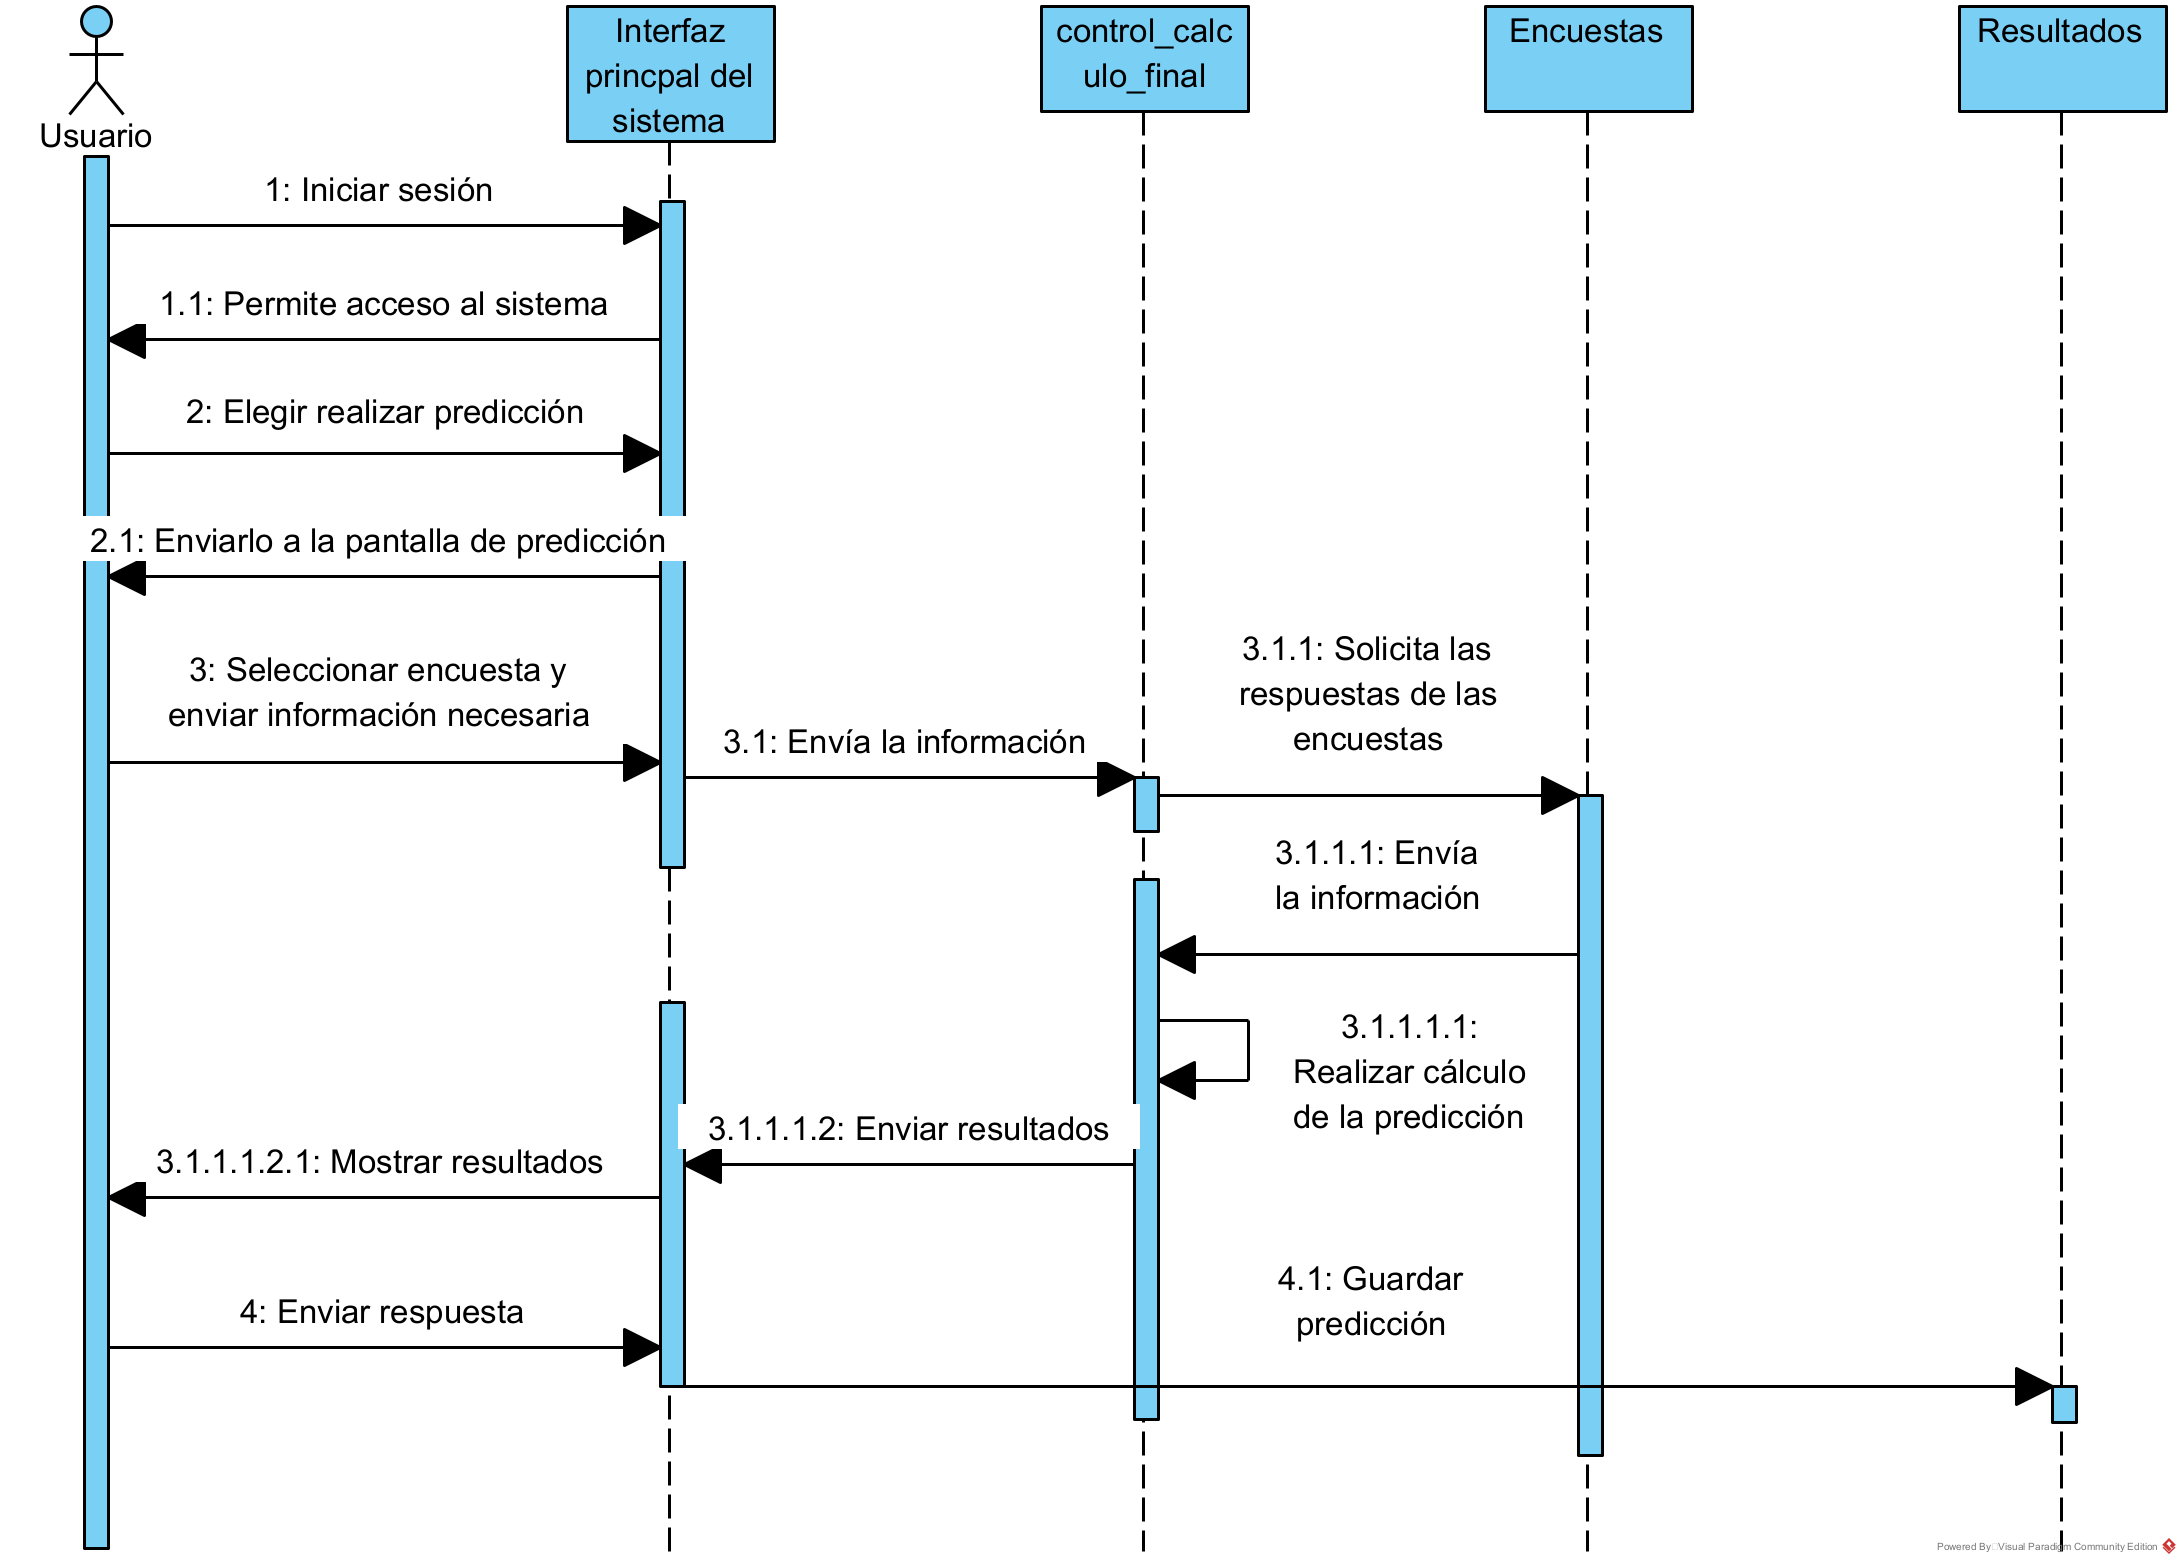
\includegraphics[scale=0.850]{TT/img/diseño/Realizar predicción.png}
    \caption{Diagrama de secuencia: Realizar predicción}
    \label{graphic:DS-Realizar predicción}
\end{figure}

\subsubsection{Descripción del flujo de información}

\begin{enumerate}
    \item Para realizar la predicción el usuario ingresa al sistema con su usuario y contraseña.
    \item El sistema verificará que los datos ingresados sean correctos, de ser así, permite el acceso al sistema.
    \item El usuario navegará a la sección de realizar predicción.
    \item El sistema le mostrará la página para realizar la predicción.
    \item El usuario seleccionará alguna encuesta creada por él y llenará los campos necesarios para realizar la predicción.
    \item La información enviada a través de la interfaz, será transferida al modulo de cálculo de predicción del servidor.
    \item El módulo de predicción solicita las respuestas de la encuesta a la base de datos.
    \item La base de datos envía las respuestas de la encuesta solicitadas.
    \item El módulo hará la predicción con los datos proporcionados.
    \item Los resultados son enviados a la interfaz gráfica.
    \item La interfaz desplegará la información recibida al usuario.
    \item El usuario decidirá si desea guardar los resultados en la base de datos o de lo contrario puede volver al paso 5.
    \item Si el usuario decidió guardar los resultados, estos se guardarán en la base de datos.
\end{enumerate}

\section{Diagramas de estado}

\subsection{Realizar predicción}
El diagrama siguiente muestra la transición de estados que se da al momento de realizar el cálculo de la predicción, el nodo negro representa el punto inicial.

\begin{figure}[!ht]
    \centering
    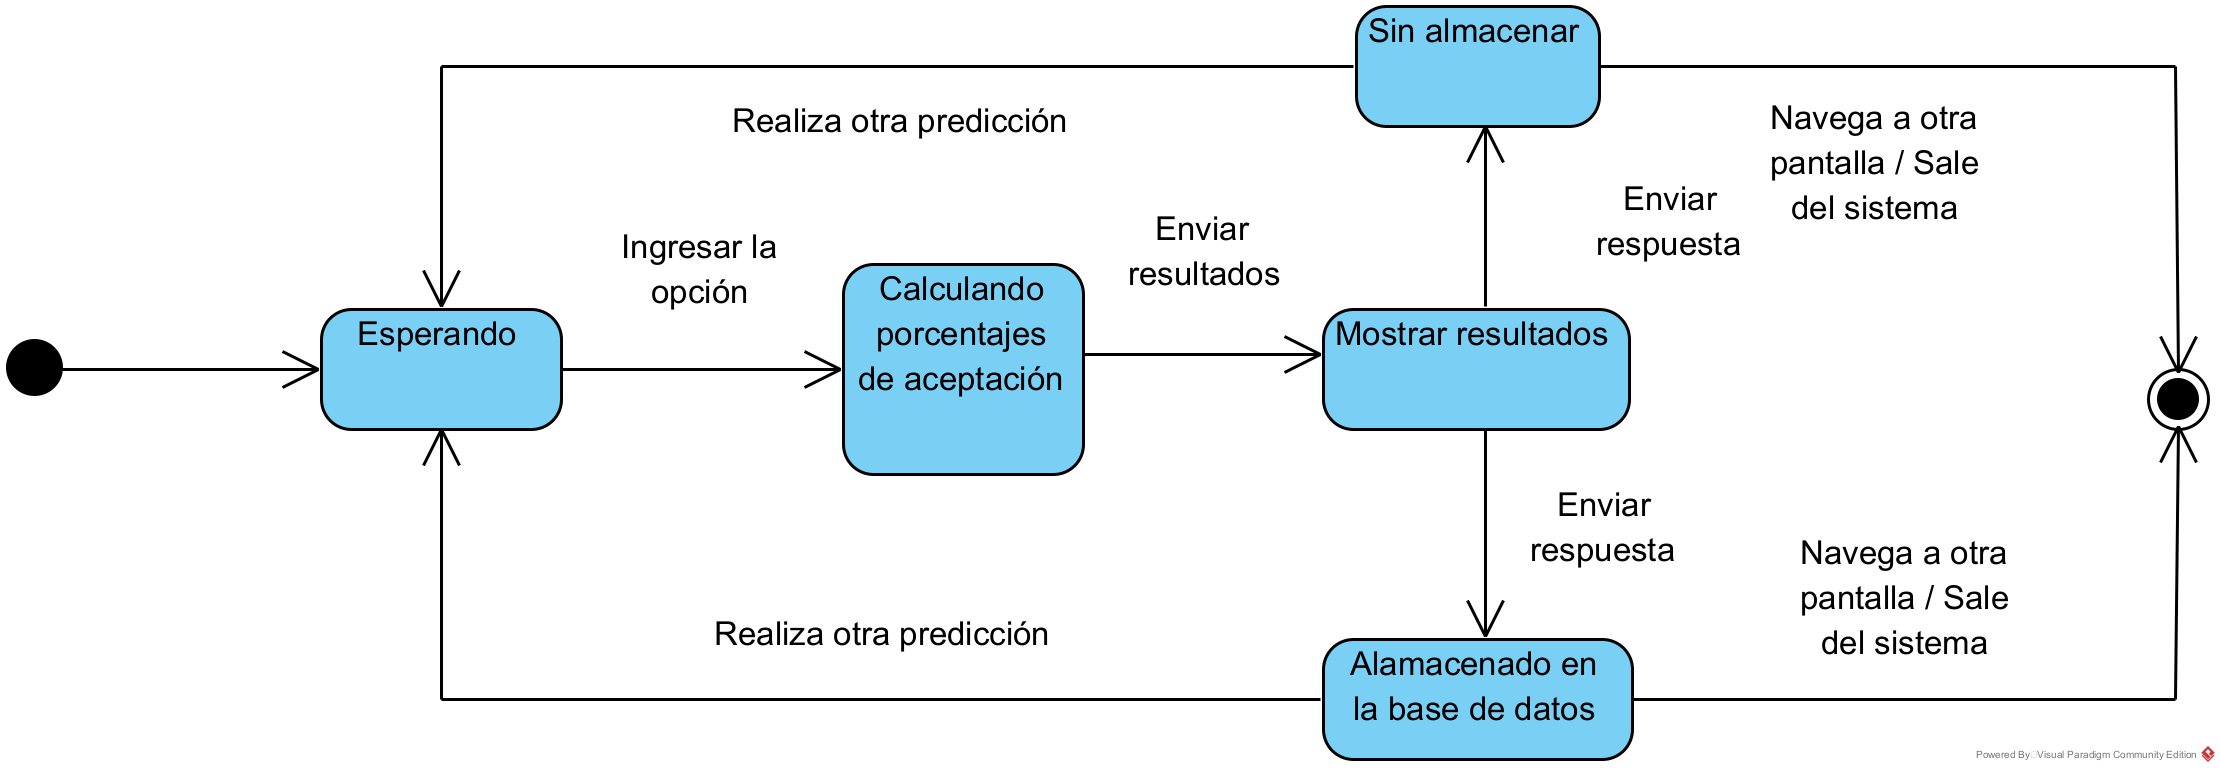
\includegraphics[scale=0.850]{TT/img/diseño/Realizar predicción DS.png}
    \caption{Diagrama de estado: Realizar predicción}
    \label{graphic:DE-Realizar predicción}
\end{figure}

\subsubsection{Descripción de estados: Realizar predicción}
\begin{enumerate}
    \item \textbf{Esperando: }En este estado, la interfaz gráfica de usuario espera a que el usuario elija una opción para la predicción.
    \item \textbf{Calculando porcentajes de aceptación: }Se calculan los porcentajes de éxito y fracaso.
    \item \textbf{Mostrar resultados: }El módulo de control envía los resultados a la interfaz gráfica y esta los muestra.
    \item \textbf{Sin almacenar: }No se almacenan los datos en la base de datos.
    \item \textbf{Almacenado en la base de datos: }Los datos son guardados.
    \item El ciclo de estados termina volviendo a realizar una predicción o saliendo de la pantalla de predicción o del sistema.
\end{enumerate}

\section{Diagrama de actividades}

\subsection{Realizar predicción}
El siguiente diagrama muestran las actividades que se realizan en el cálculo de la predicción así como el control de su flujo. El nodo negro indica un inicio y el nodo negro encerrado dentro de otra circunferencia indica el punto final.

\begin{figure}[!ht]
    \centering
    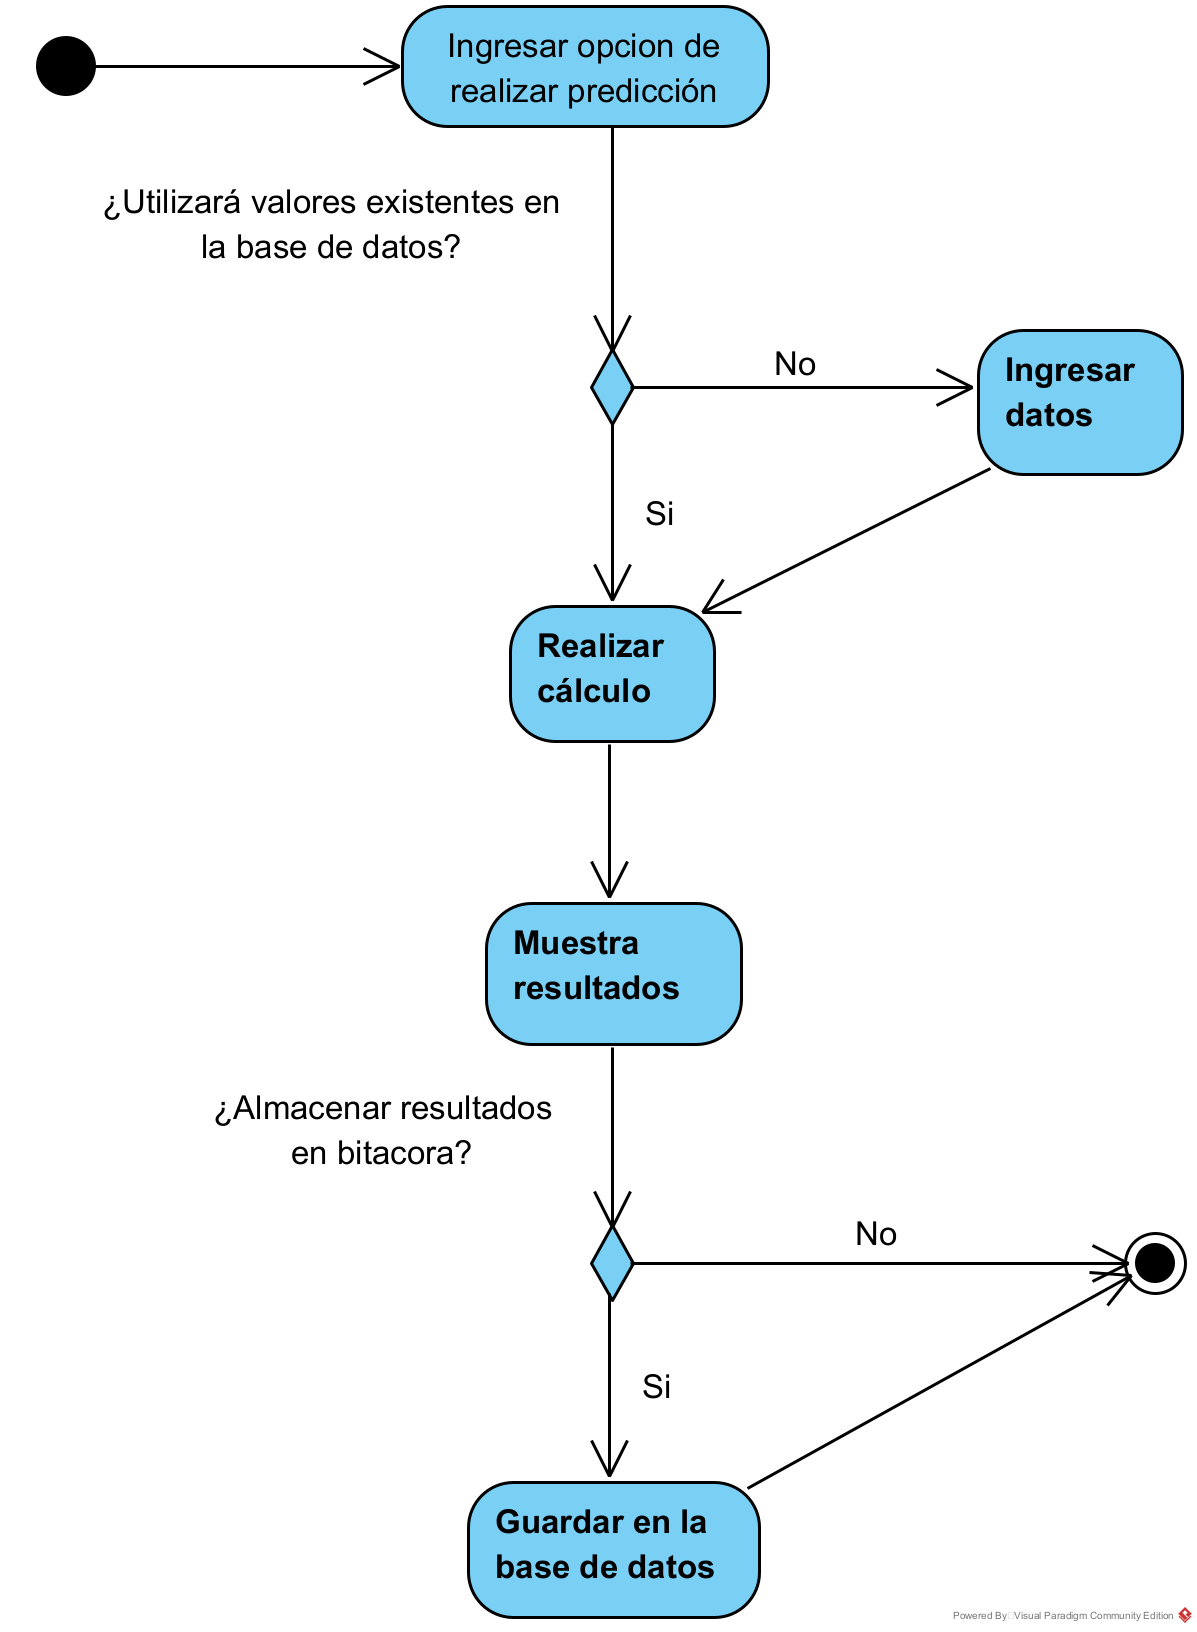
\includegraphics[scale=0.850]{TT/img/diseño/Realizar predicción DA.png}
    \caption{Diagrama de actividad: Realizar predicción}
    \label{graphic:DA-Realizar predicción}
\end{figure}

\section{Diagrama de clases}
En la figura \ref{graphic:DC-SISPREL} se muestra el diagrama de clases general, únicamente se muestran los atributos, las relaciones y las operaciones elementales.

\begin{figure}[!ht]
    \centering
    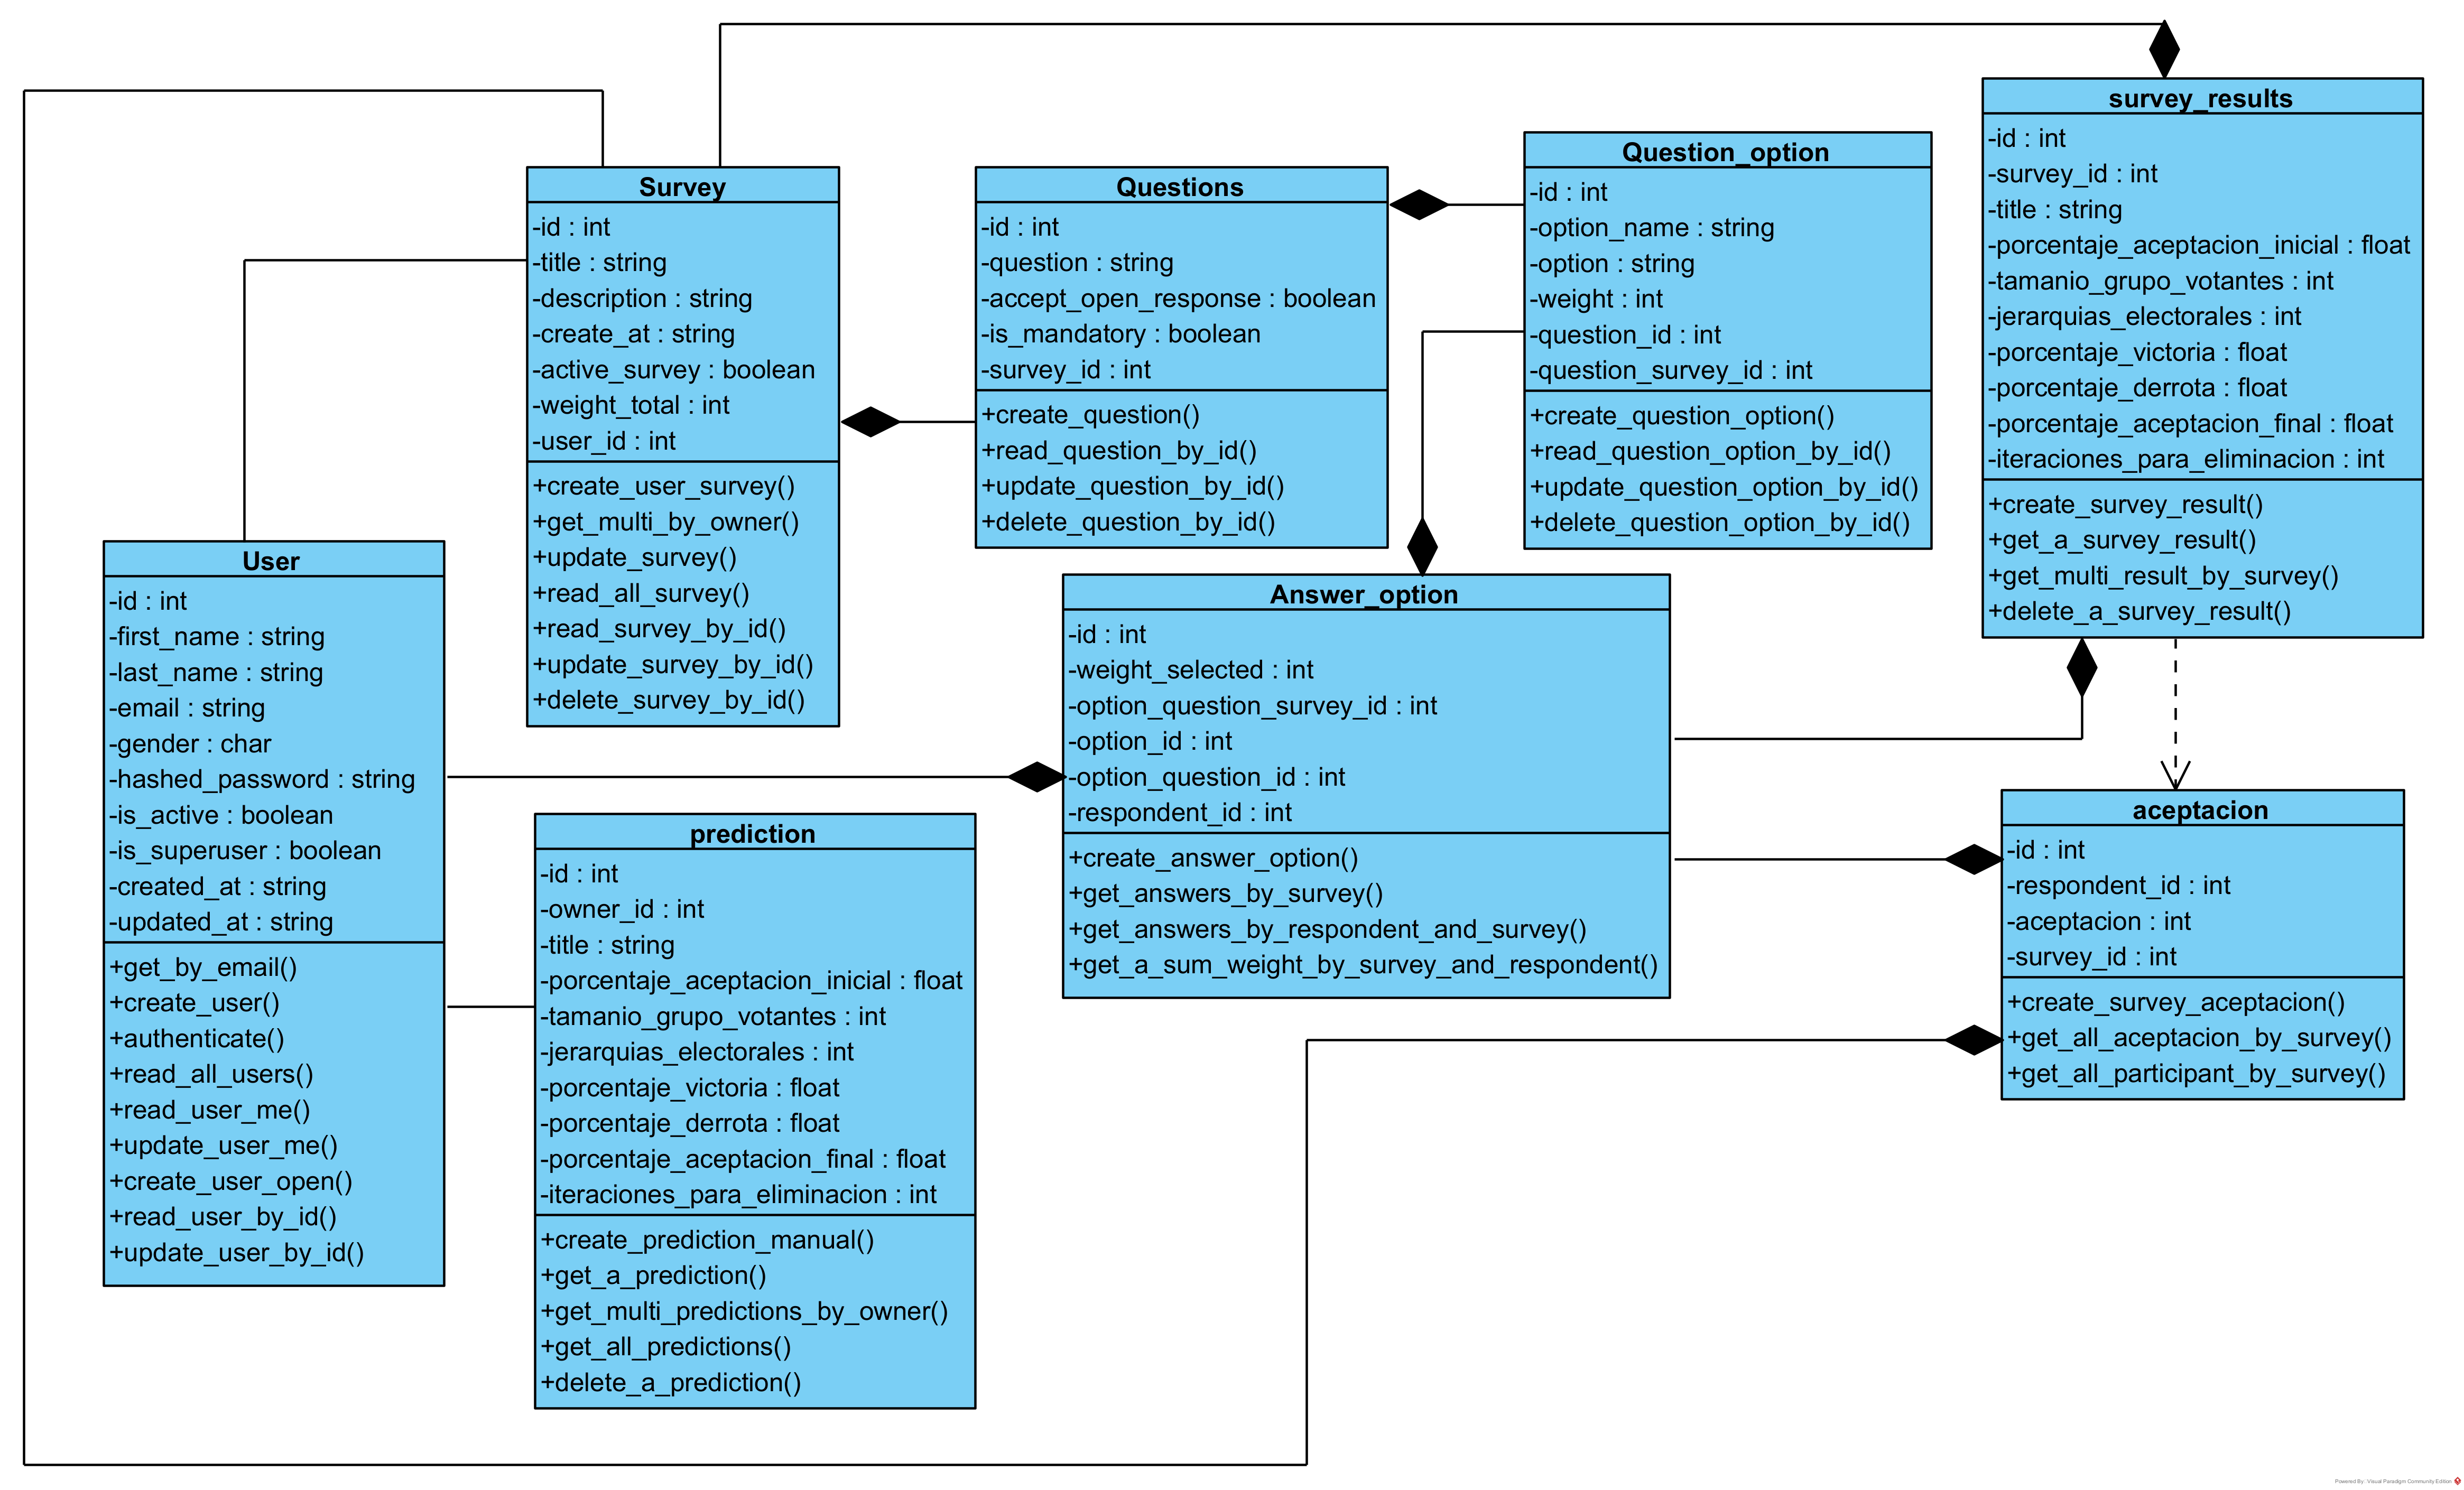
\includegraphics[scale=0.40]{TT/img/diseño/Class Diagram_sisprel.png}
    \caption{Diagrama de clases SISPREL}
    \label{graphic:DC-SISPREL}
\end{figure}


\section{Diseño de bases de datos}
Para el funcionamiento de este sistema será necesaria la implementación de una base de datos, para guardar los datos de los usuarios, las encuestas y sus respuestas.

\subsection{Diagrama de entidad relación}
SISPREL guardará los datos que están en el diagrama \ref{graphic:entidad-relación} de entidad-relación.

\begin{figure}[!ht]
    \centering
    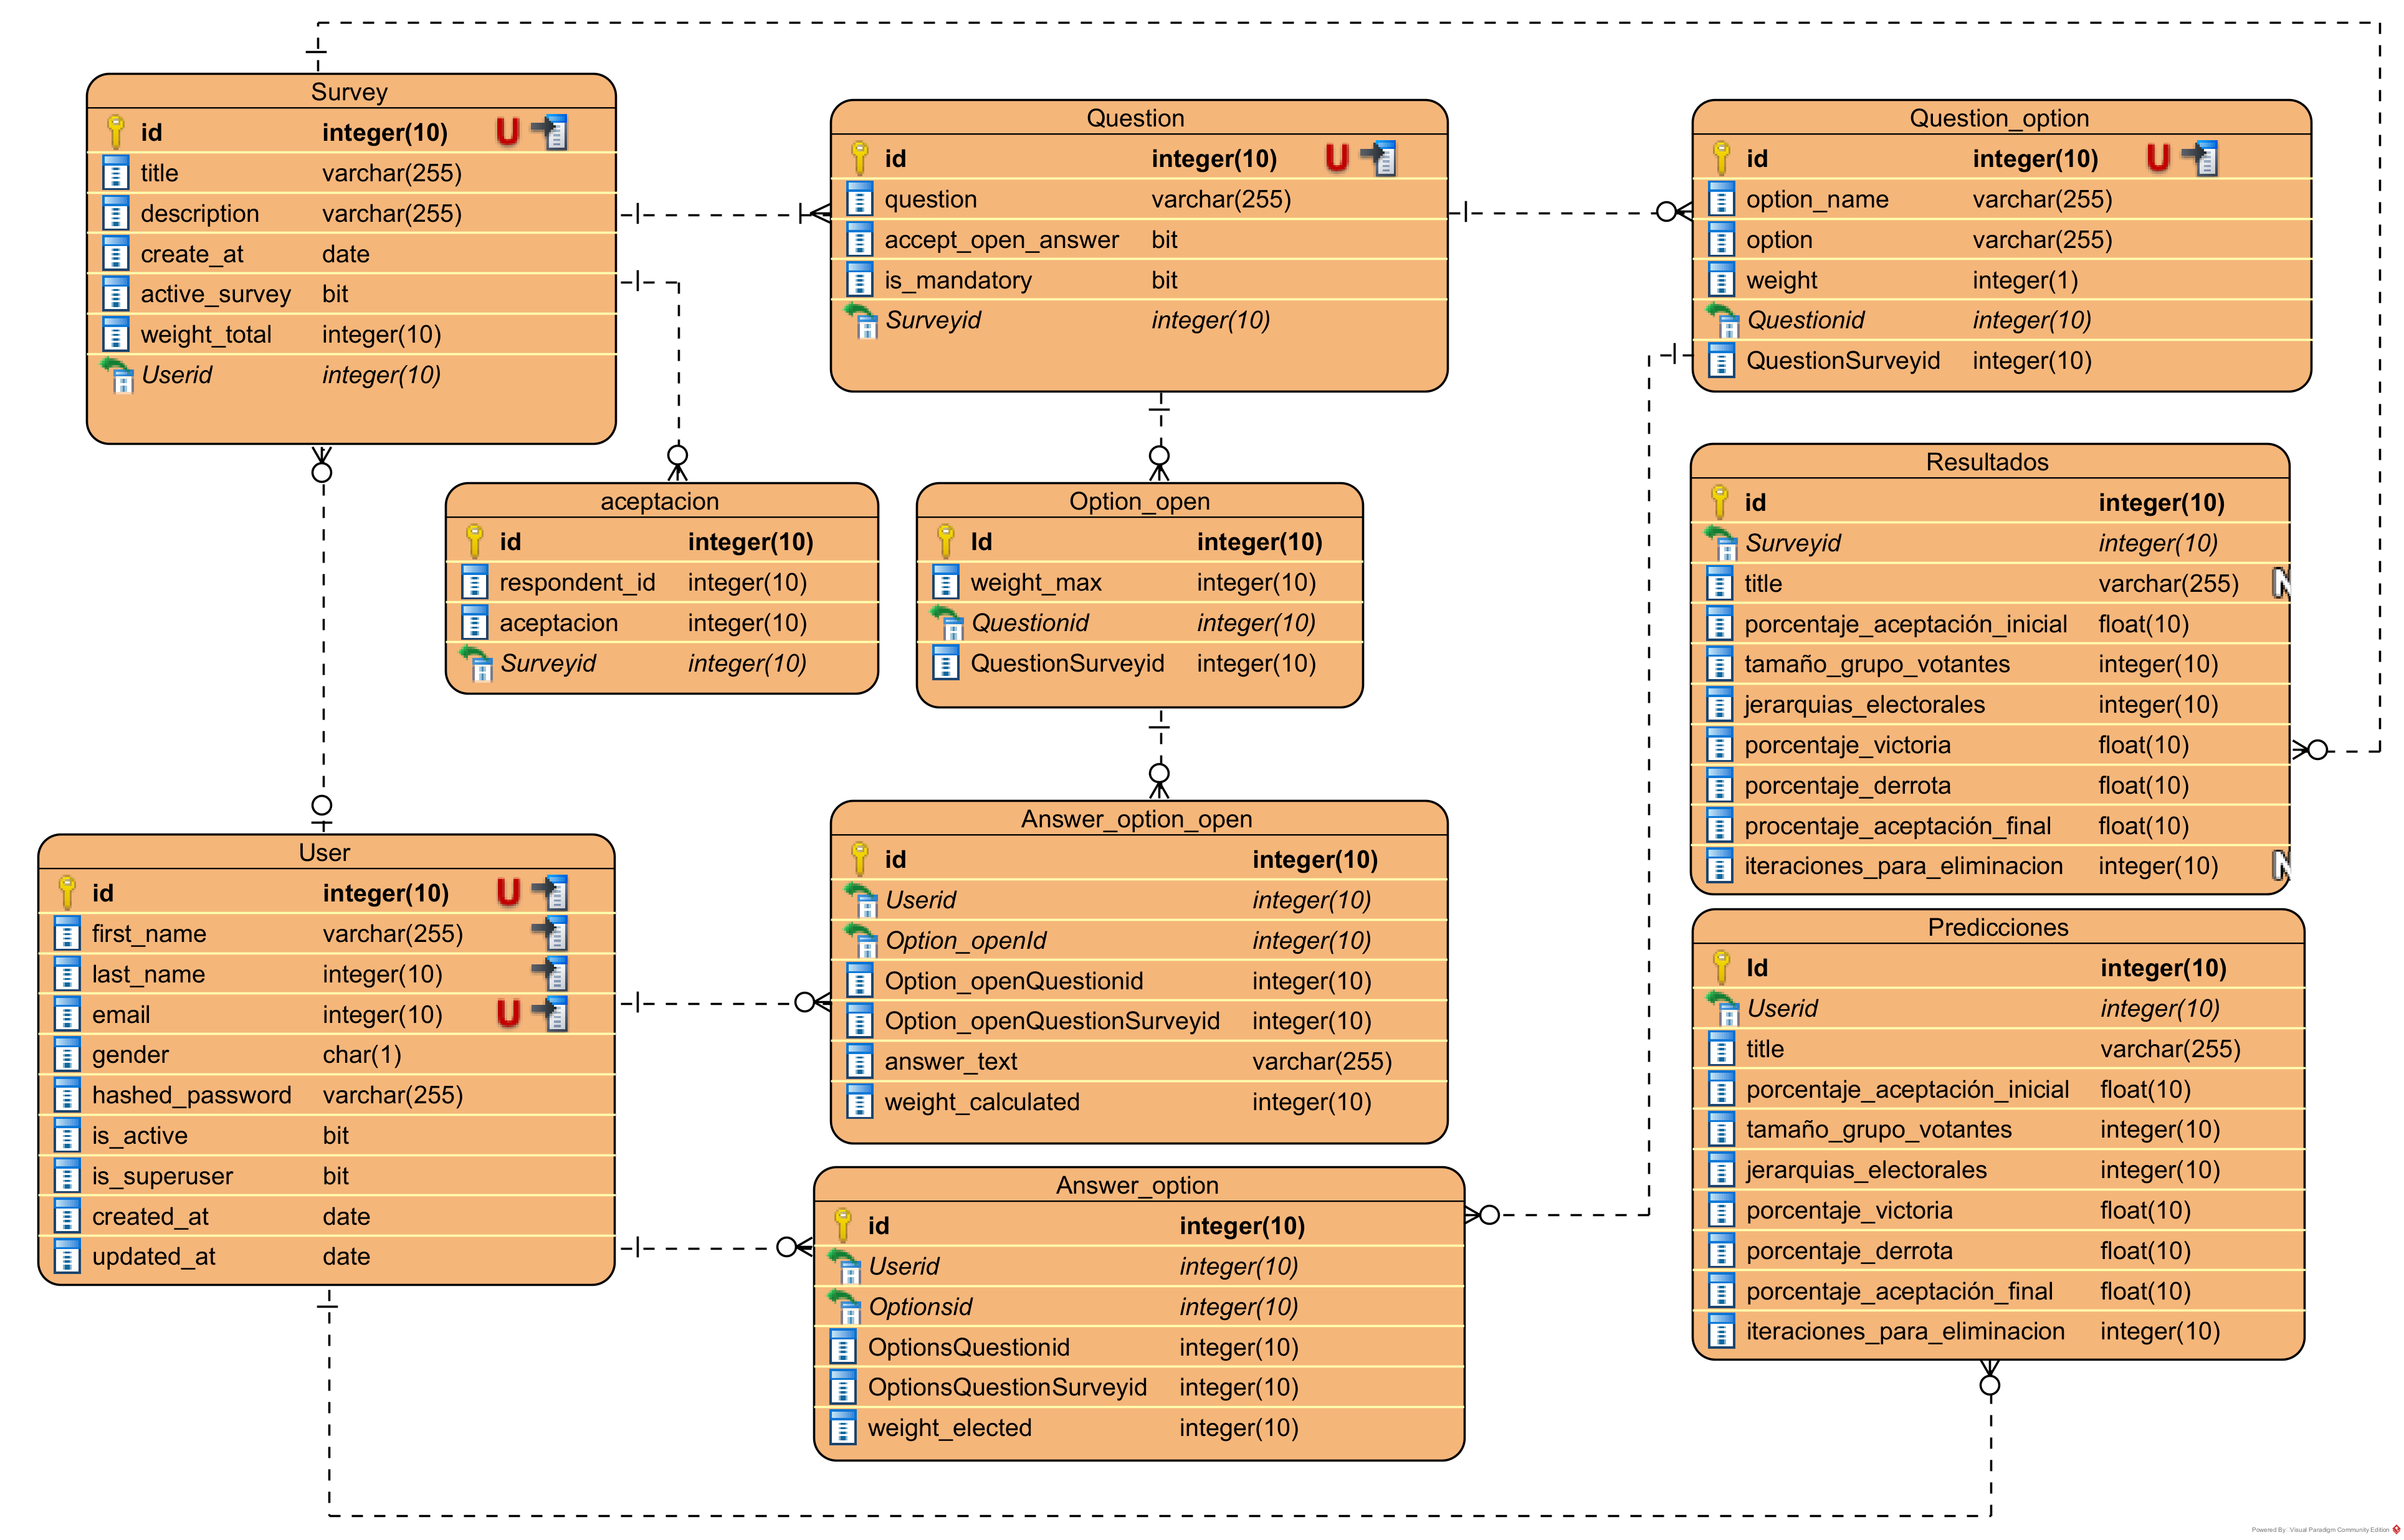
\includegraphics[scale=0.450]{TT/img/diseño/SISPREL.png}
    \caption{Diagrama entidad-relación de SISPREL}
    \label{graphic:entidad-relación}
\end{figure}

\section{Diagrama de arquitectura general del sistema}
En la figura \ref{graphic:arquitectura-sisprel} se detalla a grandes rasgos el funcionamiento principal de SISPREL.
\begin{enumerate}
    \item Se recibe una petición de internet que indica el punto de acceso al que se necesita acceder, esta petición contiene los parámetros necesarios (token, tipo de petición, datos en formato JSON) para que esta sea cumplida.
    \item La petición es recibida por el contenedor, el cual se encarga de dirigirlo a la API.
    \item La API procesa la petición mediante los módulos que esta contiene.
    \item Una vez procesada la API se encarga de realizar las operaciones correspondientes a la base de datos.
    \item La base de datos guarda y/o entrega los datos solicitados.
    \item La API procesa los datos otorgados por la base de datos y los envía al usuario.
\end{enumerate}

\begin{figure}[!ht]
    \centering
    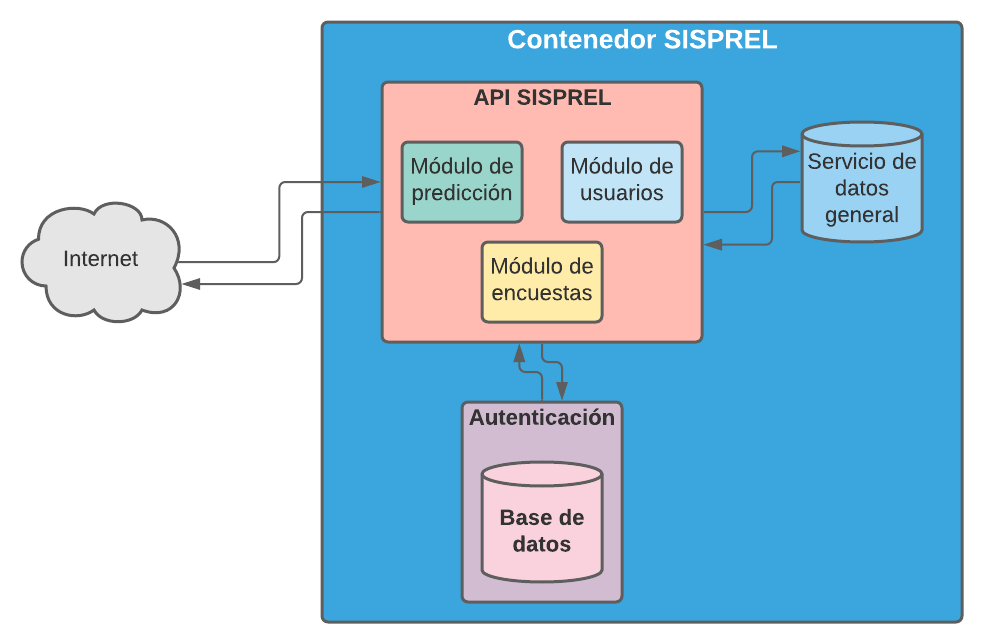
\includegraphics[scale=0.450]{TT/img/diseño/Diagrama-bloques-sisprel.png}
    \caption{Diagrama de arquitectura general de SISPREL}
    \label{graphic:arquitectura-sisprel}
\end{figure}

%\subsection{Modelo relacional}
\chapter{Implementación} 
\epigraph{\textit{I believe that at the end of the century the use of words and general educated opinion will have altered so much that one will be able to speak of machines thinking without expecting to be contradicted.     
	}}{\textit{—  Alan Turing, Computing machinery and intelligence}}
	\vspace*{8cm}
	\begin{center}
		\centering
		\includegraphics[width=10.5cm]{example-image}
	\end{center}
	\thispagestyle{empty}
	\newpage
\vspace*{2cm}

\section{Desarrollo de logo}
Se presenta el logo de SISPREL.
\begin{figure}[!htb]
    \centering
    
\includegraphics[scale=0.25]{TT/img/sisprel.png}
    \caption{Logo de SISPREL}
    \label{graphic:SISPRELLogo}    
\end{figure}

\section{Estructura del proyecto}
Para tener un control del proyecto, se presenta a continuación la estructura general con la cual se ha trabajado para tener una buena organización del sistema y sea fácil de entender donde va cada módulo del sistema, mas adelante se ahondará mas en cada sección del sistema.

\begin{enumerate}
    \item Frontend: En esta carpeta se almacenarán los módulos y el proyecto del Frontend del sistema, será desarrollado con JavaScript con el Framework VueJS
    \item Backend: En esta carpeta se almacenará el entorno de Python con los paquetes y el sistema desarrollado.
    \item Scripts: En esa carpeta se encontrarán los Scripts necesarios para construir y levantar de manera local el contenedor o subirlo en algun servicio en la nube.
    \item Raíz: En la carpeta raíz o donde se encuentran las carpetas mencionadas anteriormente, se encuentran algunos archivos de configuración de los contenedores asi mismo un archivo .env donde se almacenan variables como puertos, contraseña, URLs y otras cosas para que los archivos de configuración de Docker los usen y al momento de modificar alguna variable solo se tenga que hacer en un solo archivo y de manera general.
\end{enumerate}

\begin{figure}[!htb]
    \centering
    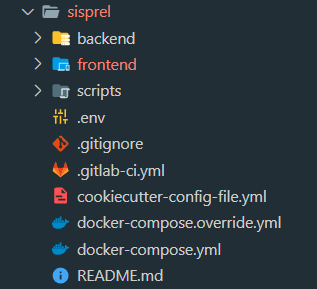
\includegraphics[scale=0.95]{TT/img/implementacion/carpetasGeneral.png}
    \caption{Estructura general de SISPREL}
    \label{graphic:carpetasGeneral}    
\end{figure}


\section{Configuración del entorno del sistema}
Para el desarrollo del sistema y poder trabajarlo en cualquier lugar sin tener que hacer instalaciones o configuraciones para cada sistema operativo, se optó por usar contenedores. Para ello, se eligió el software de Docker para llevar acabo este fin. 

El proyecto fue dividido en 4 contenedores, los cuales son:
\begin{enumerate}
    \item Proxy: Traefik 2.2
    \item DB: Postgres 12
    \item Backend: FastAPI
    \item Frontend: VueJS
\end{enumerate}

\subsection{Traefik}
Traefik es un enrutador/proxy inverso y un balanceador HTTP, TCP y UDP. Una herramienta que permite conectar distintas URL con el servicio que se requiera. Proporciona funcionalidades de intermediario que aumenta sus capacidades para realizar balanceo de carga o servir como gateway API. Además integra una Interfaz de usuario muy completa que nos da información sobre todo lo que ofrece. Para acceder a esta herramienta en el proyecto, de manera local se accede con la URL: localhost:8090.

\begin{figure}[!htb]
    \centering
    
\includegraphics[scale=0.1]{TT/img/implementacion/Traefik.logo.png}
    \caption{Logo de Traefik}
    \label{graphic:TraefikLogo}    
\end{figure}

Sus principales características son:
\begin{itemize}
    \item \textbf{Enrutado y balanceo de carga: }capa de enrutado flexible en la capa 4 y 7, soporta los protocolos HTTP, HTTP/2, TCP, UDP, Websockets, gRPC, despliegues blue-green y canary, fijación de sesión o session stickness y comprobaciones de salud.
    \item \textbf{Seguridad: }automatización de HTTP, soporte para Let’s Encrypt, certificados personalizados y autenticación.
    \item \textbf{Configuración dinámica: }a través de descubrimiento de servicios (Kubernetes, Docker Swarm, Red Hat OpenShift, Rancher, Amazon ECS, key-value stores) y funcionales de intermediario o middelware (circuit breakers, reintentos, buffering, compresión de la respuesta, cabeceras o limitación de peticiones).
    \item \textbf{Observabilidad: }posee un panel informativo de forma nativa, trazabilidad distribuida (Jaeger, Open Tracing, Zipkin) y métricas en tiempo real (Datadog, Grafana, InfluxDB, Prometheus, StatsD).
\end{itemize}

\begin{figure}[!htb]
    \centering
    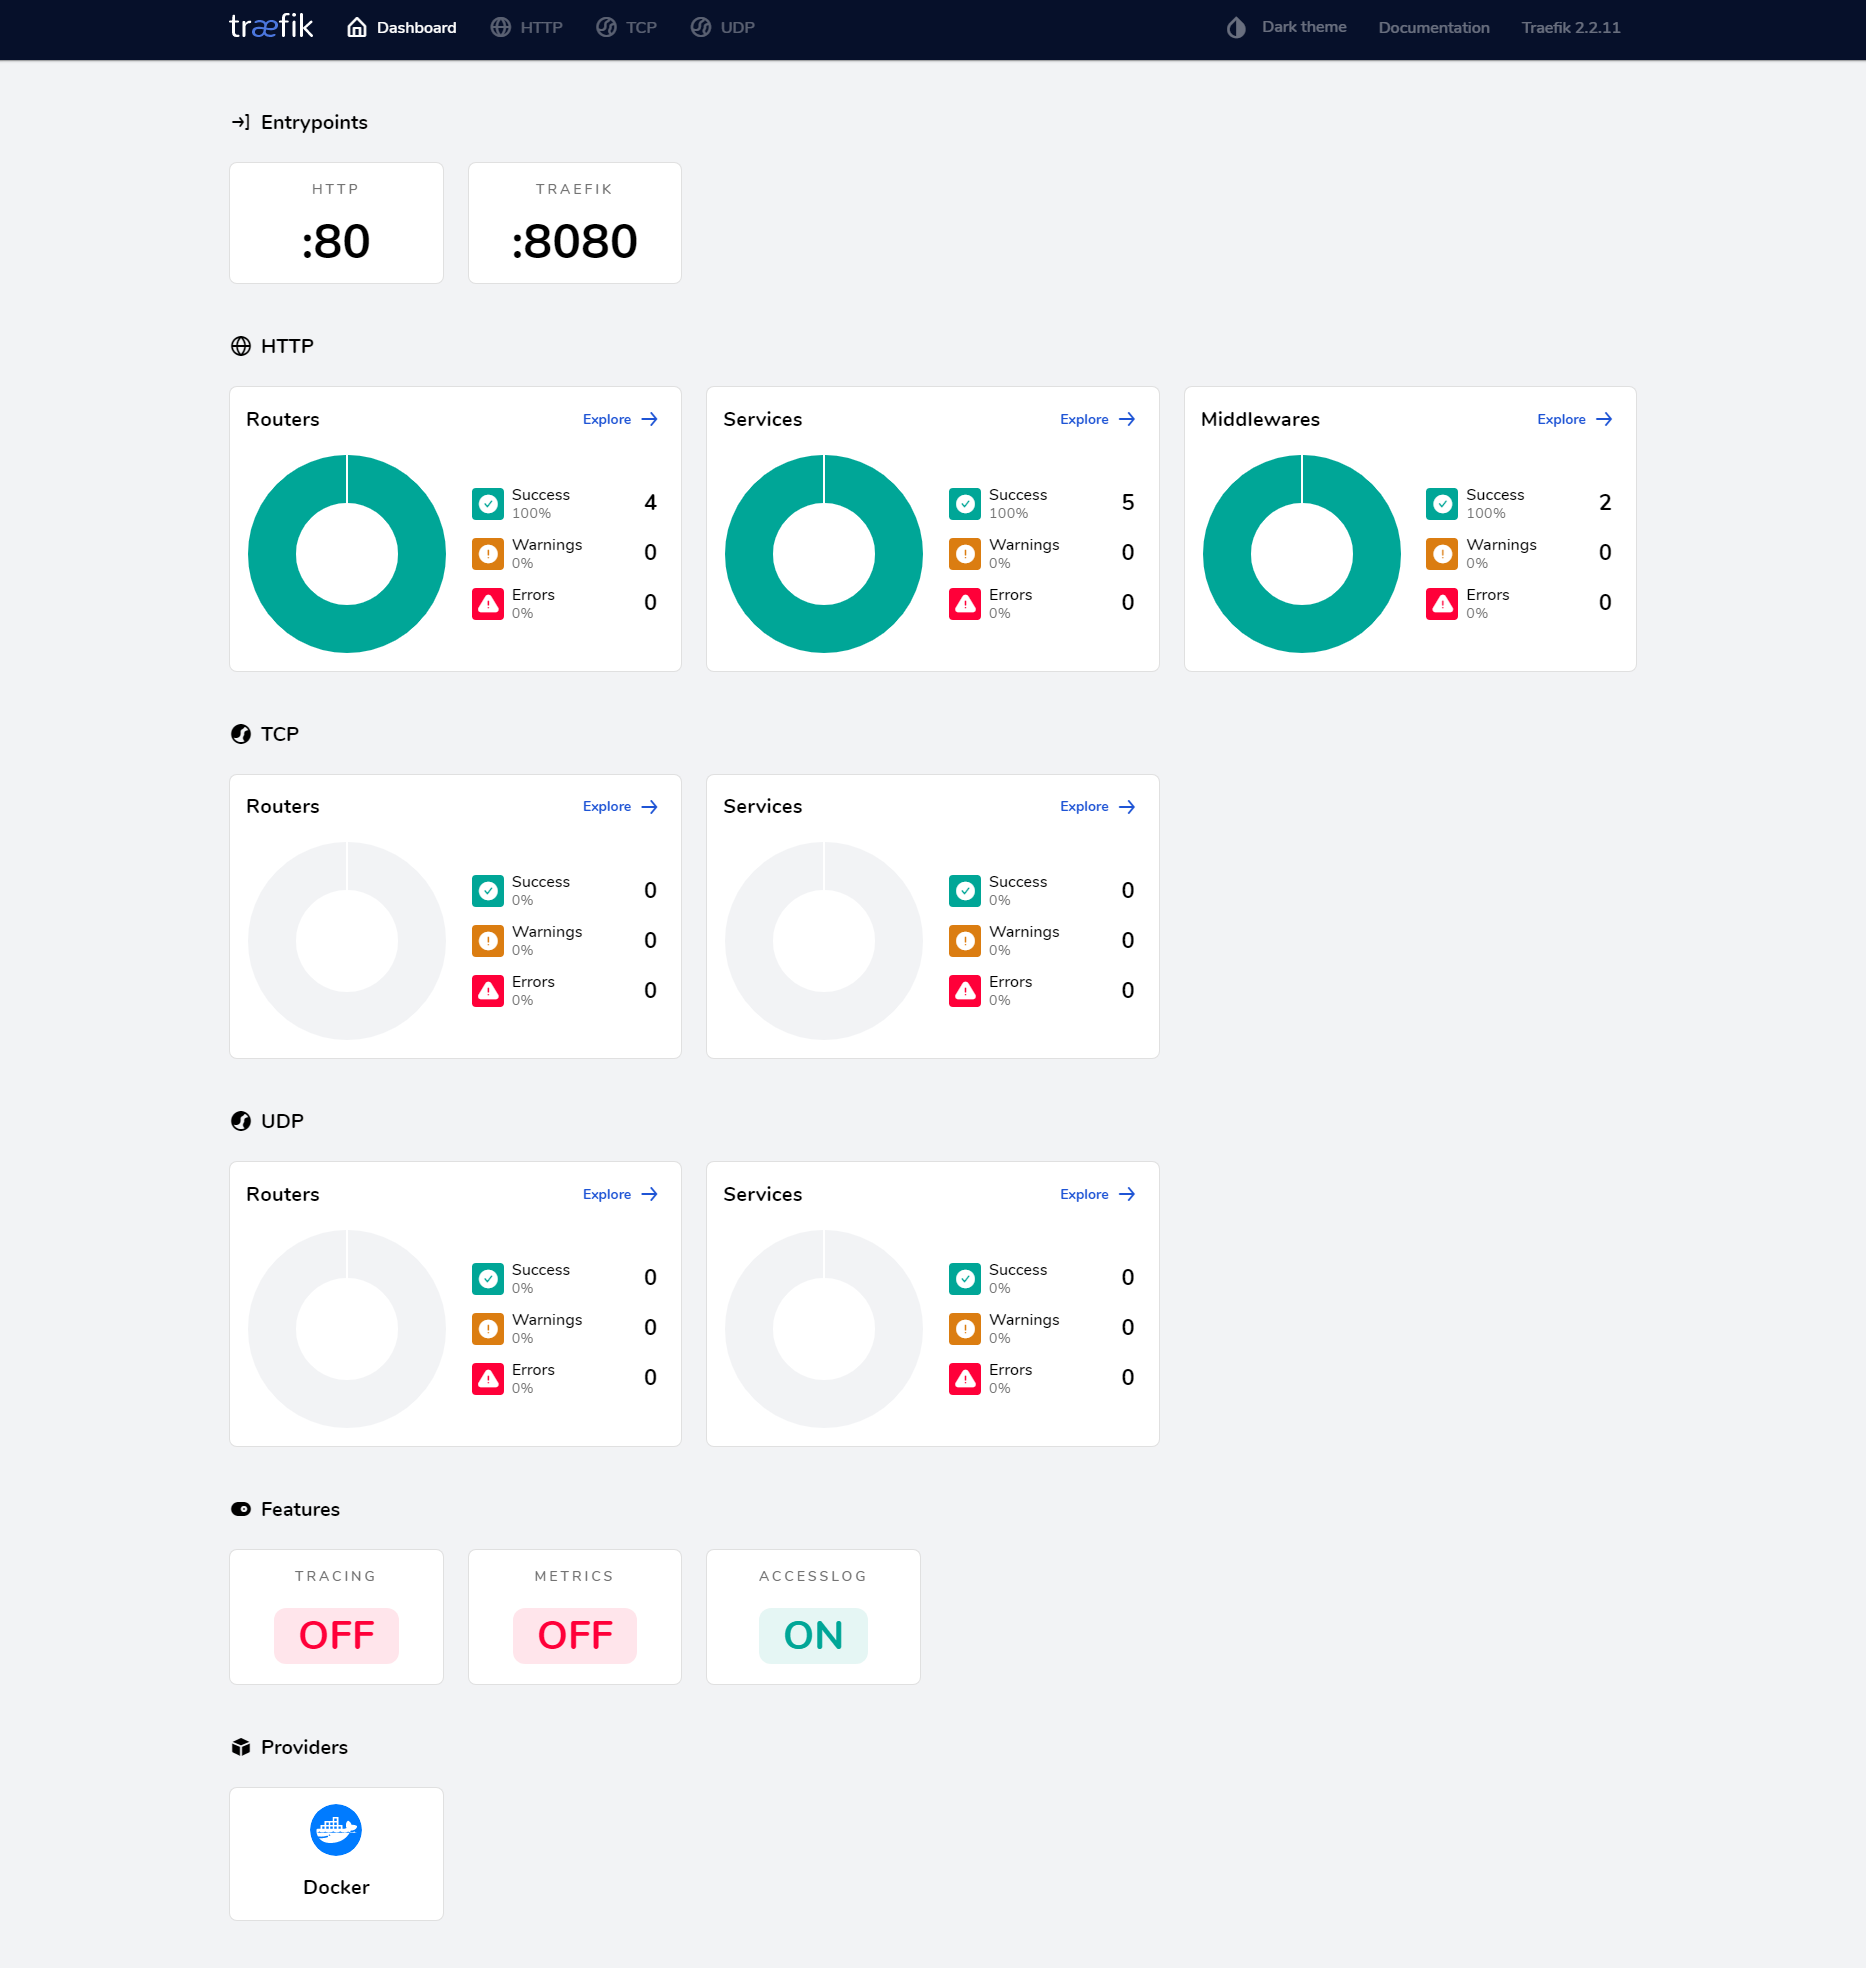
\includegraphics[scale=0.2]{TT/img/implementacion/Traefik dashboard.png}
    \caption{Dashboard de Traefik}
    \label{graphic:TraefikDashboard}    
\end{figure}

\subsection{Postgres}
Postgres es la herramienta elegida de base de datos para el sistema. Se eligió por ser 100\% OpenSource. También cuenta con una imagen de docker con la cual se ha configurado y trabajado para realizar el sistema.

\subsection{FastAPI}
Continuamos con FastApi, es una herramienta que ayuda a desarrollar API's de manera rápida basada en Python. Se usó una imagen de Python en su versión 3.9 en docker. A continuación se describirá el proceso de desarrollo de la API usando estas herramientas.

\subsubsection{Preparando entorno de desarrollo}
Para tener un control de los paquetes que vamos a usar, se ha elegido la herramienta Poetry, la cual nos ayuda a ordenar los paquetes a usar y que facilita la instalación de estos mismos en cualquier entorno en donde se despliegue el contenedor del sistema.

Primero crearemos nuestro proyecto usando Poetry para ir instalando las dependencias que se requieren para que la API funcione correctamente. Las dependencias son: 
\begin{itemize}
    \item fastapi = "\^0.68.1"
    \item SQLAlchemy = "\^1.4.25"
    \item uvicorn = "\^0.15.0"
    \item python-dotenv = "\^0.19.0"
    \item python-multipart = "\^0.0.5"
    \item python-jose = \{extras = [cryptography], version ="\^3.3.0"\}
    \item passlib = "\^1.7.4"
    \item pydantic = \{extras = [email], version ="\^1.8.2"\}
    \item alembic = "\^1.7.3"
    \item inflect = "\^5.3.0"
    \item bcrypt = "\^3.2.0"
    \item SQLAlchemy-Utils = "\^0.37.8"
    \item psycopg2-binary = "\^2.9.1"
    \item tenacity = "\^8.0.1"
    \item pytest = "\^6.2.5"
    \item mypy = "\^0.910"
    \item sqlalchemy-stubs = "\^0.4"
    \item flake8 = "\^3.9.2"
    \item autoflake = "\^1.4"
    \item isort = "\^5.9.3"
    \item black = "\^21.9b0"
    \item pytest-cov = "\^2.12.1"
    \item numpy = "\^1.21.4"
\end{itemize}

Los dependencias destacadas son: 
\begin{itemize}
    \item \textbf{Fastapi: }Es la dependencia que contiene el framework con el que vamos a trabajar.
    \item \textbf{SQLAlchemy: }Es una herramienta que permite trabajar las bases de datos como \gls{ORM} en Python.
    \item \textbf{Uvicorn: }Es un servidor ASGI rápido. Uvicorn se basa en uvloop y httptools y es un miembro importante del ecosistema asincrónico de Python.
    \item \textbf{Alembic: }es una herramienta de migración de bases de datos escrita por el autor de SQLAlchemy que permite versionar las bases de datos, en otras palabras, tener un historial de los cambios que se vayan realizando a la base de datos, ejemplo: cambiar el nombre de una tabla, el nombre de uno o varios atributos, las especificaciones de estos, etc.
    \item \textbf{Psycopg2-binary: }es el adaptador de base de datos PostgreSQL para el lenguaje de programación Python.
\end{itemize}

Poetry ofrece la opción de crear un entorno virtual en Python, pero como se ha configurado una imagen de Python para el desarrollo del sistema, no es necesario crear un entorno virtual para la instalación de los paquetes vistos anteriormente.

\subsubsection{Estructura de la API}
Continuemos con la estructura de la API, en esta sección se describirá las carpetas y que es lo que almacenan. En la carpeta backend se localiza el archivo de configuración de docker, con el cual se configura el entorno del contenedor y ejecutar algunos scripts. 

\textbf{Nivel 1 y 2}

En la carpeta \textit{app} que se muestra en la figura \ref{graphic:carpetasapi1} hay mas carpetas, que se visualizan en la figura \ref{graphic:carpetasapi2}. Adentro se localizan la carpeta \textit{alembic}: en esta carpeta se encuentra la herramienta que actúa como versionador de bases de datos; en la carpeta scripts hay archivos que corrigen el formato de los archivos python así como realizar test básicos del sistema; lo siguiente por explicar son los archivos que se encuentran en la raíz de \textit{app}, los cuáles son archivos de configuración para la base de datos y la lista de paquetes administrada por poetry para el entorno de trabajo; por último se encuentra otra carpeta igualmente \textit{app}, en ella se encuentran los archivos de python que conforman el sistema.

\begin{figure}[!htb]
    \centering
    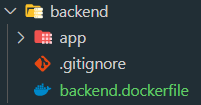
\includegraphics[scale=1]{TT/img/implementacion/carpeta-api-1.png}
    \caption{Carpetas de la API - Parte 1}
    \label{graphic:carpetasapi1}    
\end{figure}

\begin{figure}[!htb]
    \centering
    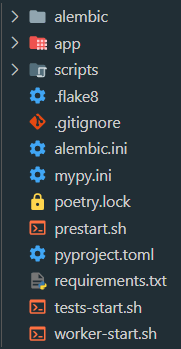
\includegraphics[scale=1]{TT/img/implementacion/carpeta-api-2.png}
    \caption{Carpetas de la API - Parte 2}
    \label{graphic:carpetasapi2}    
\end{figure}

\textbf{Nivel 3}

Continua la explicación de la carpeta \textit{app}, esta carpeta contiene los archivos del proyecto, se muestran en la figura \ref{graphic:carpetasapi3}. Iniciamos con la carpeta models, en esta carpeta se encuentran los archivos donde se han definido los modelos de la base de datos, cada tabla de la base de datos se define como una clase y dentro de cada clase se definen los atributos de las tablas, sus relaciones, tipos de atributos y características como que sea nulo, único, sea llave primaria o llave foránea, etc. Esto se muestra en la figura \ref{graphic:user_model}.

\begin{figure}[!htb]
    \centering
    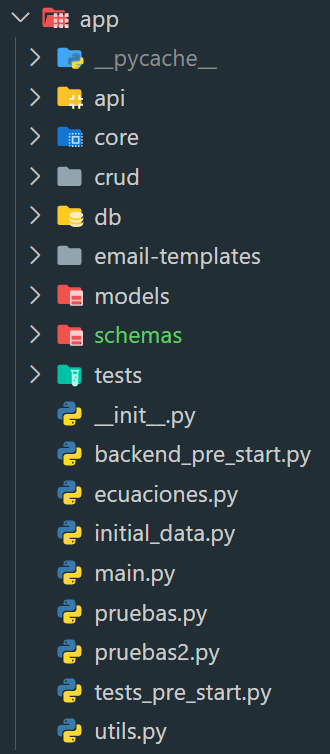
\includegraphics[scale=.9]{TT/img/implementacion/carpeta-api-3.png}
    \caption{Carpetas de la API - Parte 3}
    \label{graphic:carpetasapi3}    
\end{figure}

\begin{figure}[!htb]
    \centering
    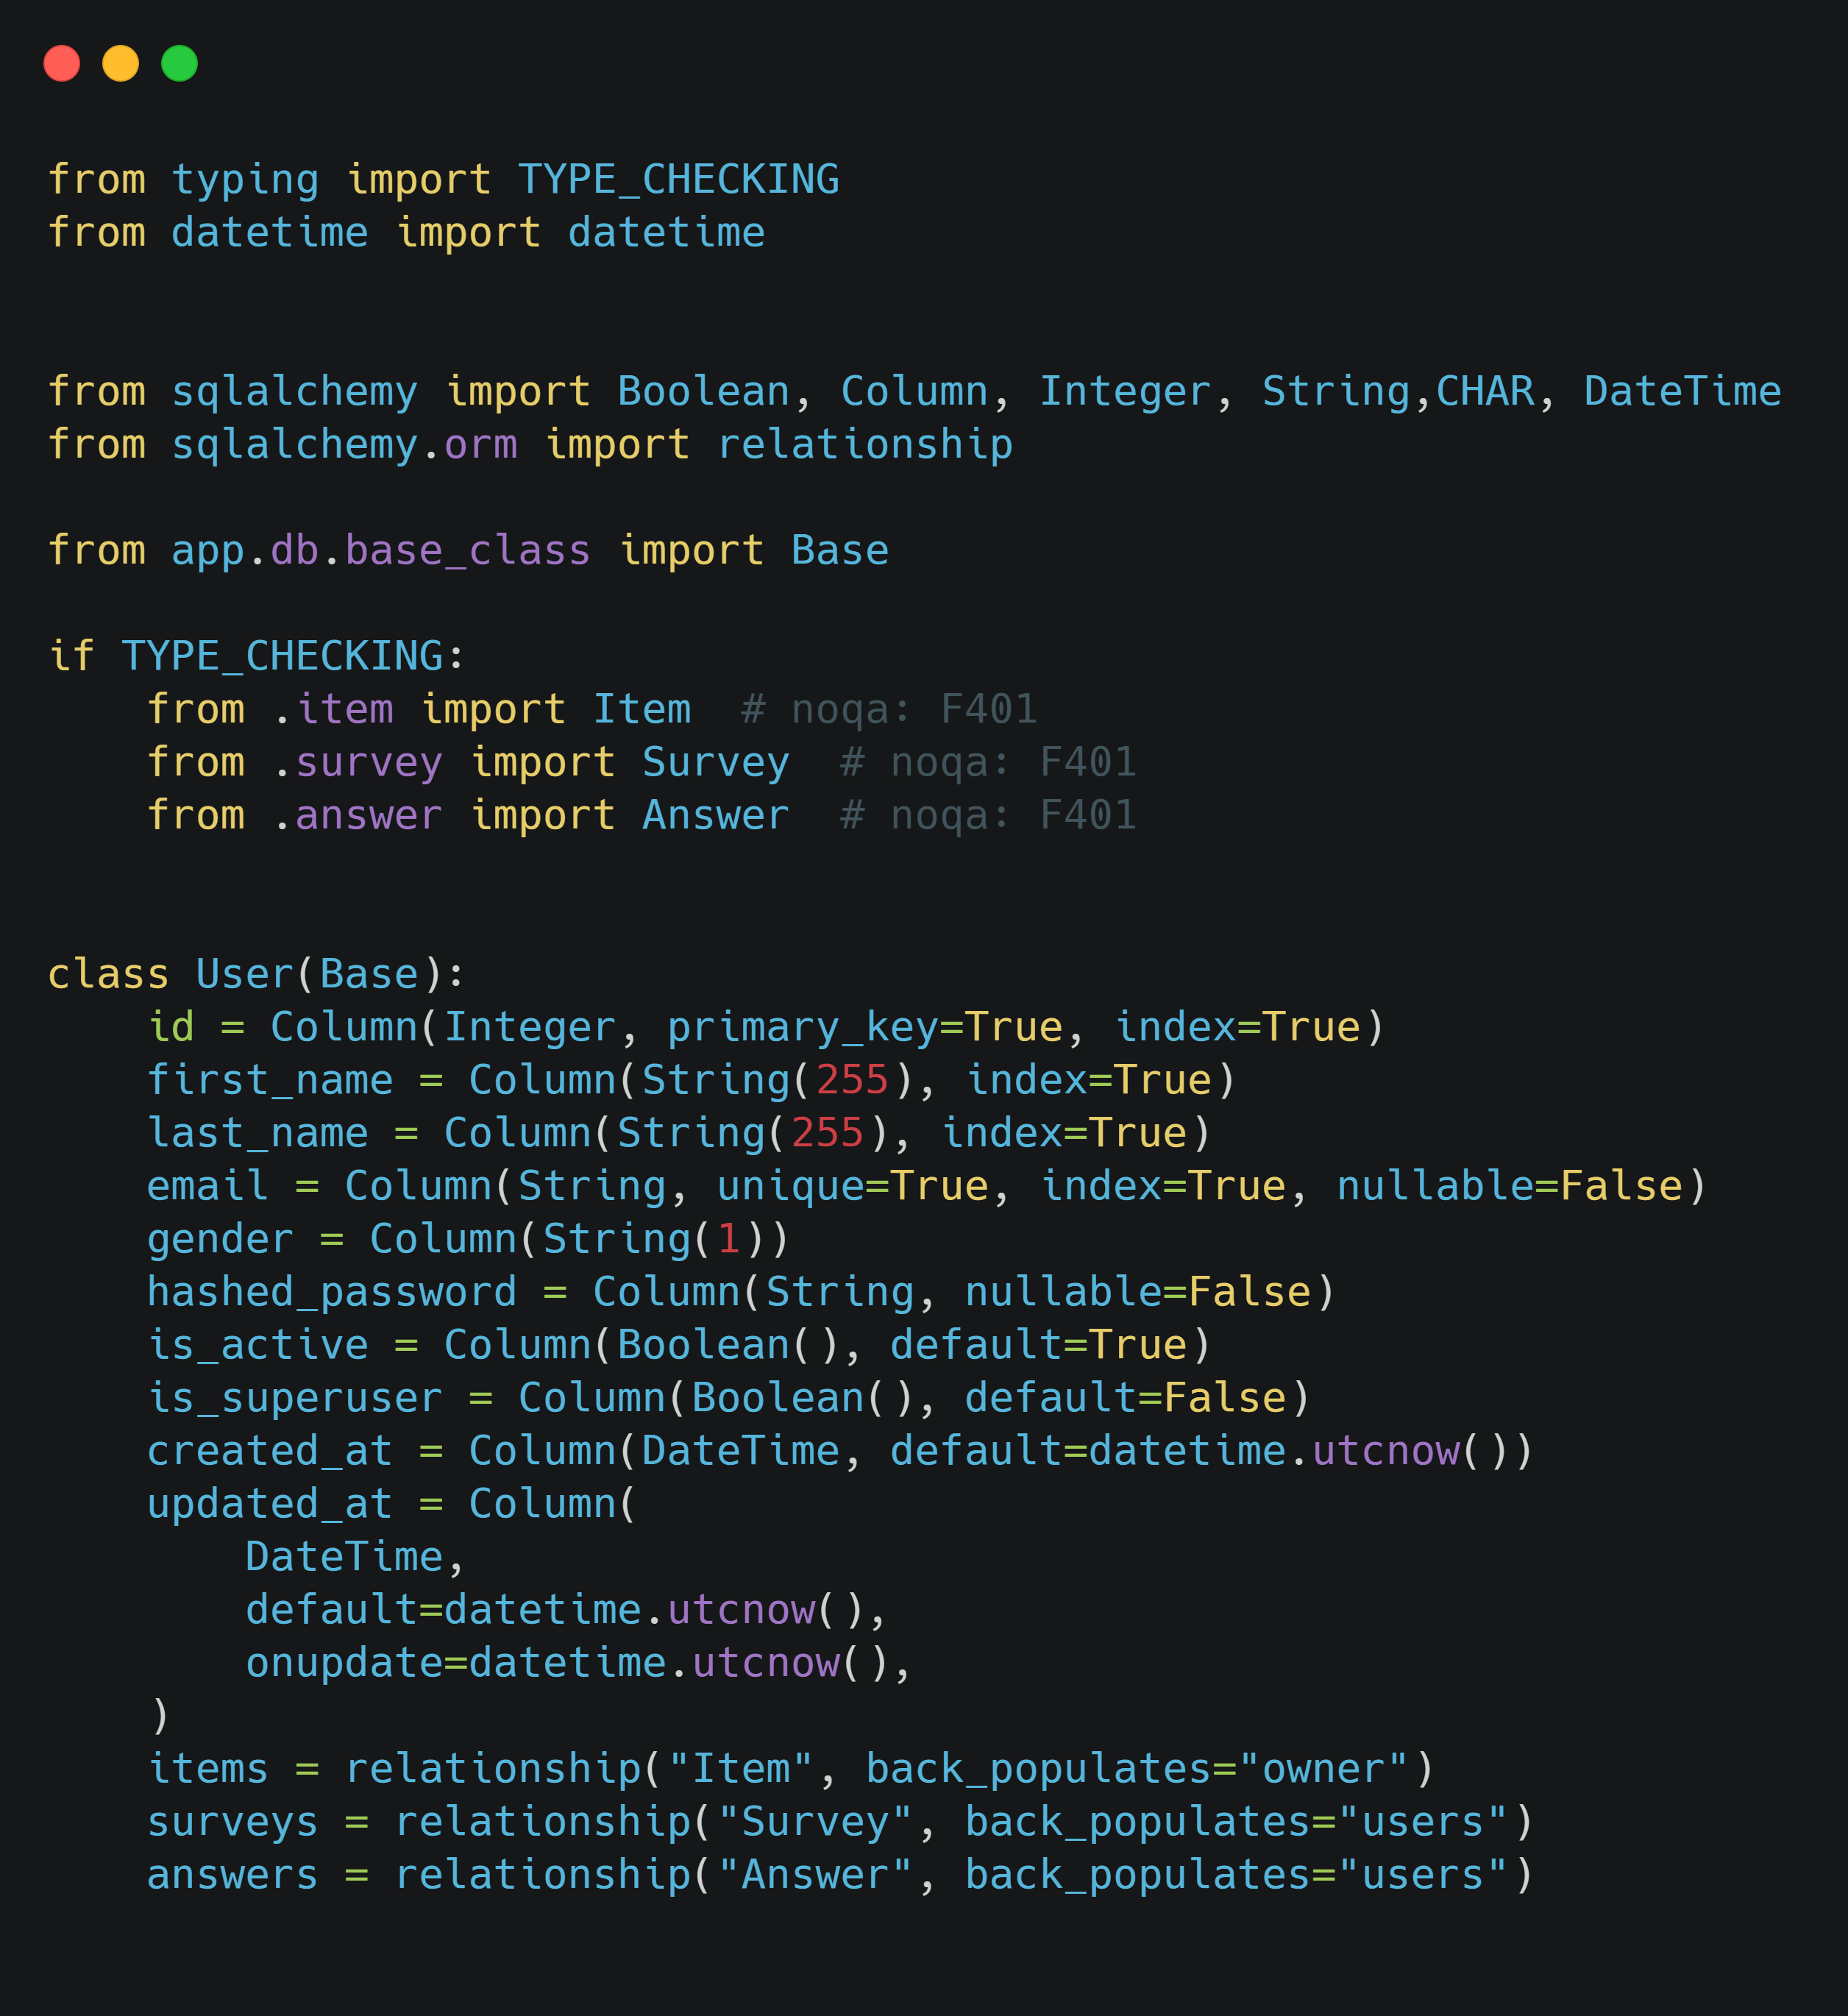
\includegraphics[scale=.15]{TT/img/implementacion/user-model.png}
    \caption{Modelo de usuario}
    \label{graphic:user_model}    
\end{figure}

Continuamos con la carpeta \textit{schemas}, dentro de esta carpeta tendremos los esquemas de los modelos de la base de datos, estos archivos nos ayudan a tener una estructura sobre los datos que son los accesibles por el usuario y cuales son los que el sistema creará de manera automática, así como el tipo de dato que van a aceptar, esto nos ayuda a que solo entren los tipos de datos que son requeridos por la base de datos lo que añade una capa de seguridad, ya que si se envían datos que no están definidos en las clases simplemente no se podrá guardar o modificar los datos guardados en la base de datos. También se define que datos son los que van a ser creados y actualizados, en la figura \ref{graphic:user_schema} donde se muestra el esquema para la tabla usuario.

\begin{figure}[!htb]
    \centering
    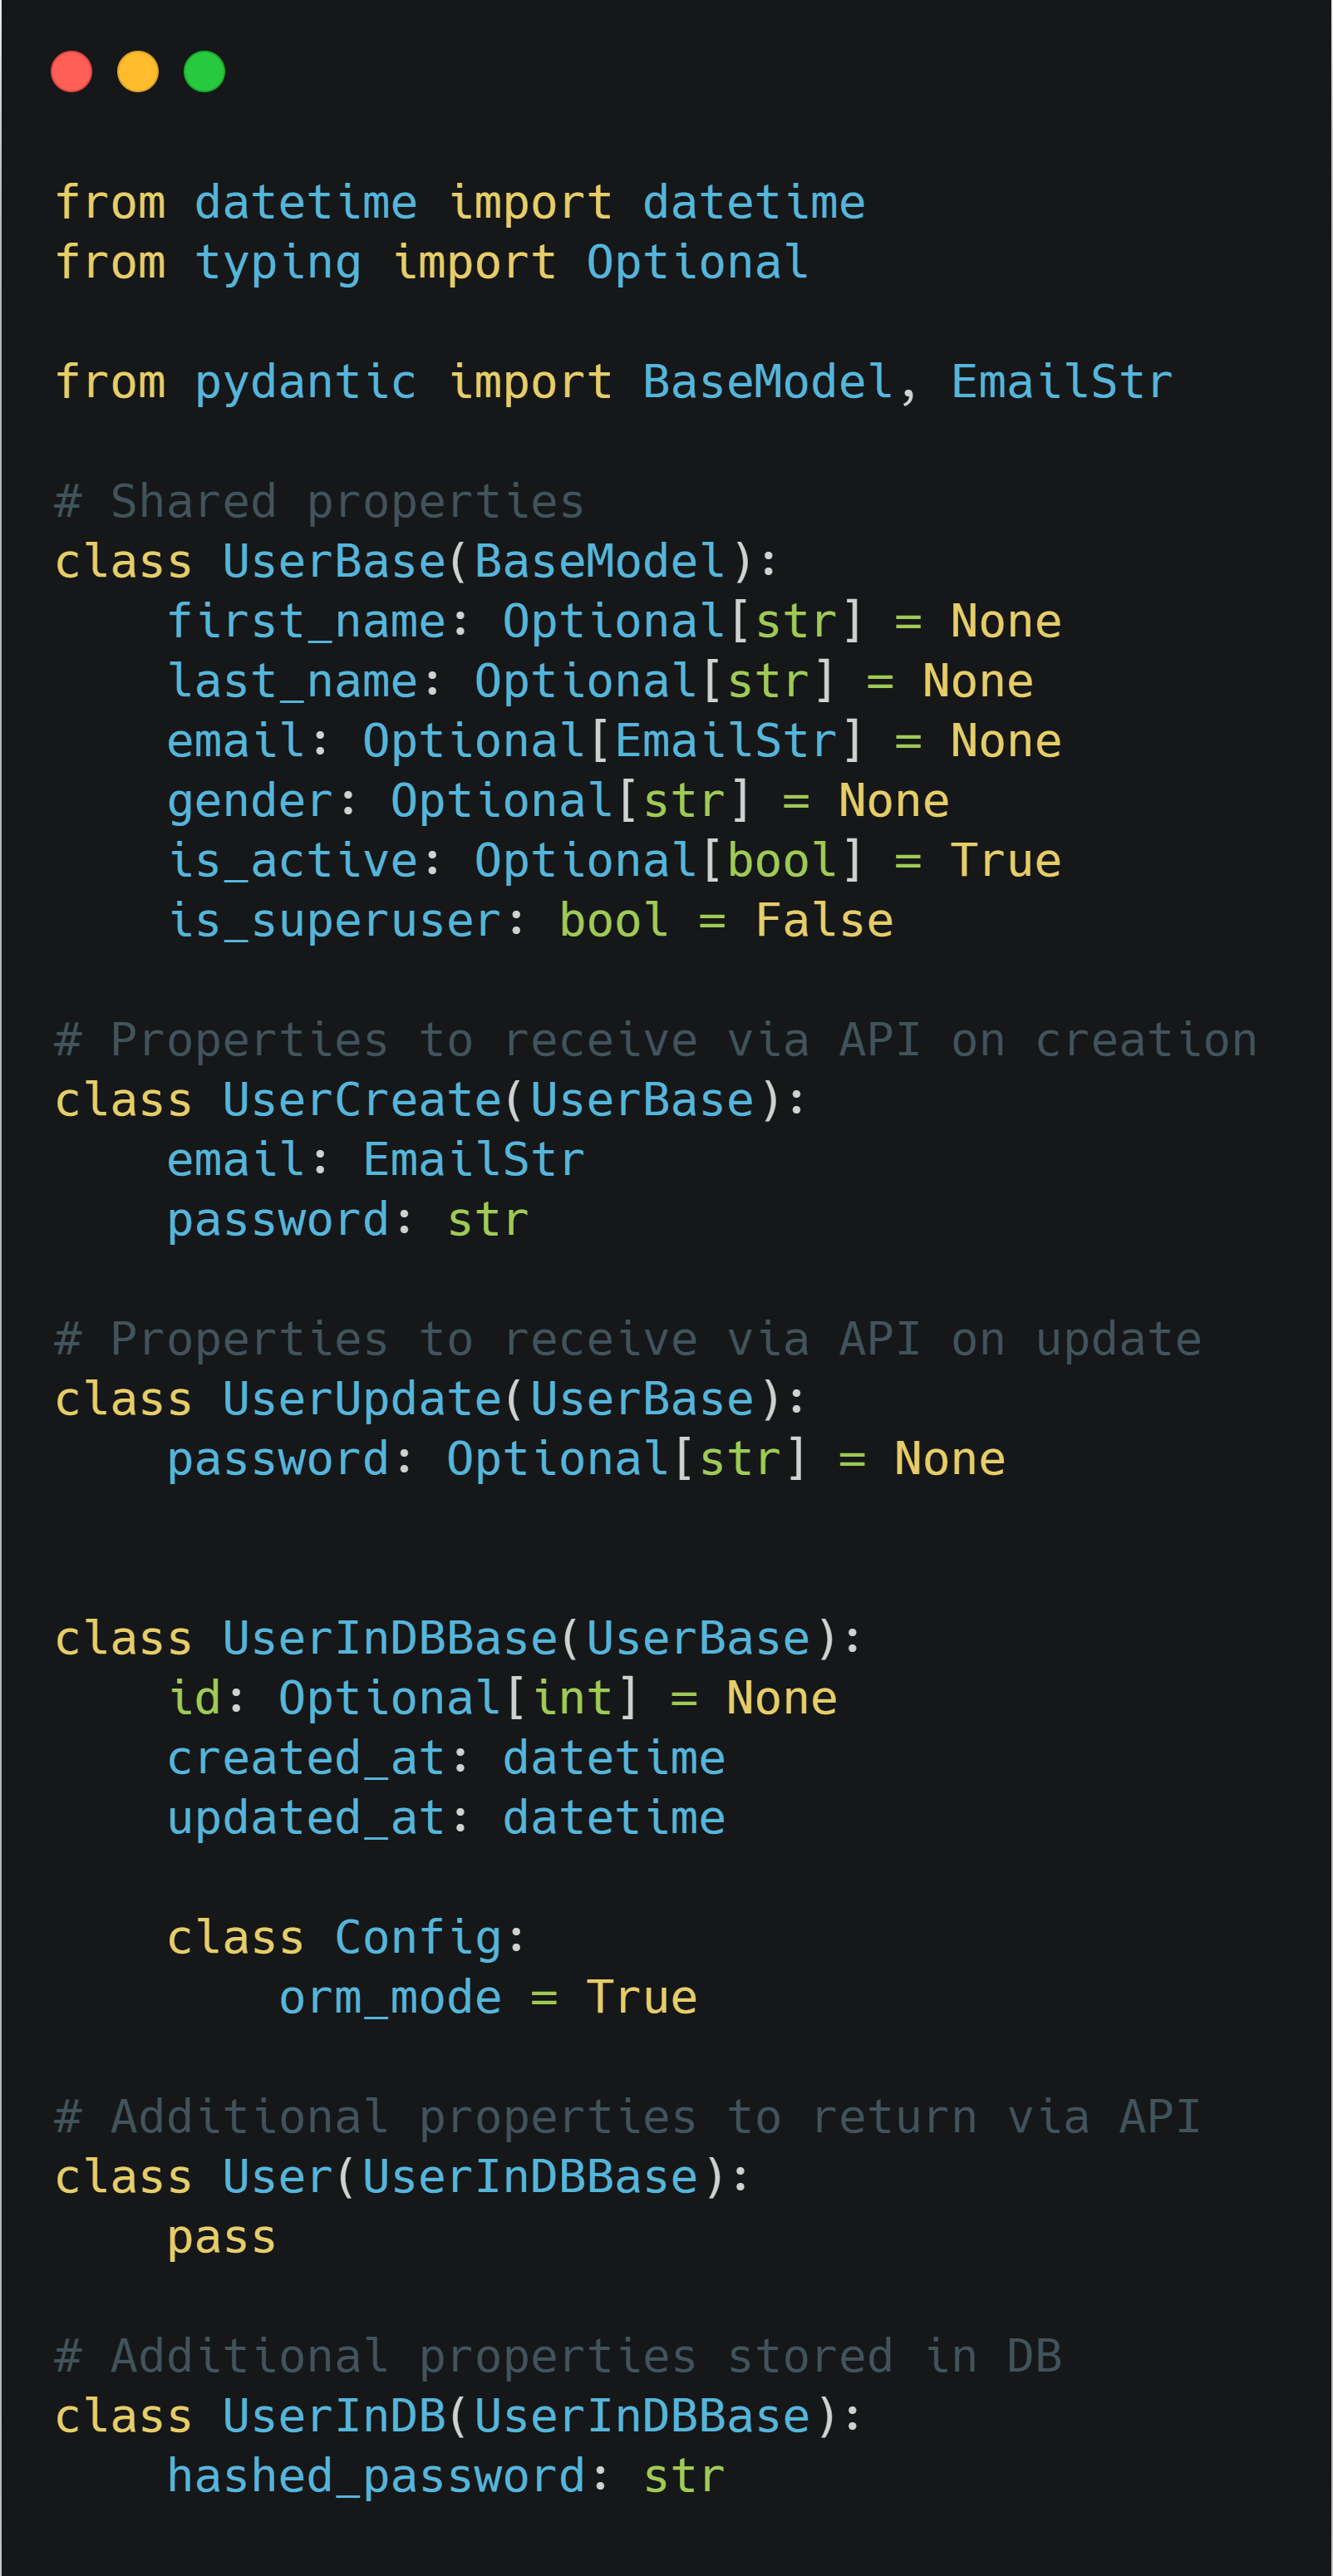
\includegraphics[scale=.15]{TT/img/implementacion/schema-user.png}
    \caption{Esquema de usuario}
    \label{graphic:user_schema}    
\end{figure}

La siguiente carpeta a presentar es \textit{crud}, en esta carpeta se encuentra el CRUD de cada tabla de la base de datos, se define un CRUD base, donde se definen las funciones básicas de crear, leer, actualizar y eliminar un elemento de la base de datos. Para complementar las funciones básicas, se han creado archivos para cada tabla en la base de datos, ya que se han requerido otras funciones, por ende, estos archivos heredan las funciones básicas ya mencionadas anteriormente, algunos ejemplos son los que se encuentran en el CRUD de usuario que se muestran en la figura \ref{graphic:user_crud} donde se aprecian funciones para buscar usuarios mediante el correo electrónico, autenticar un usuario u obtener si el usuario se encuentra activo o es un súper-usuario.

\begin{figure}[!htb]
    \centering
    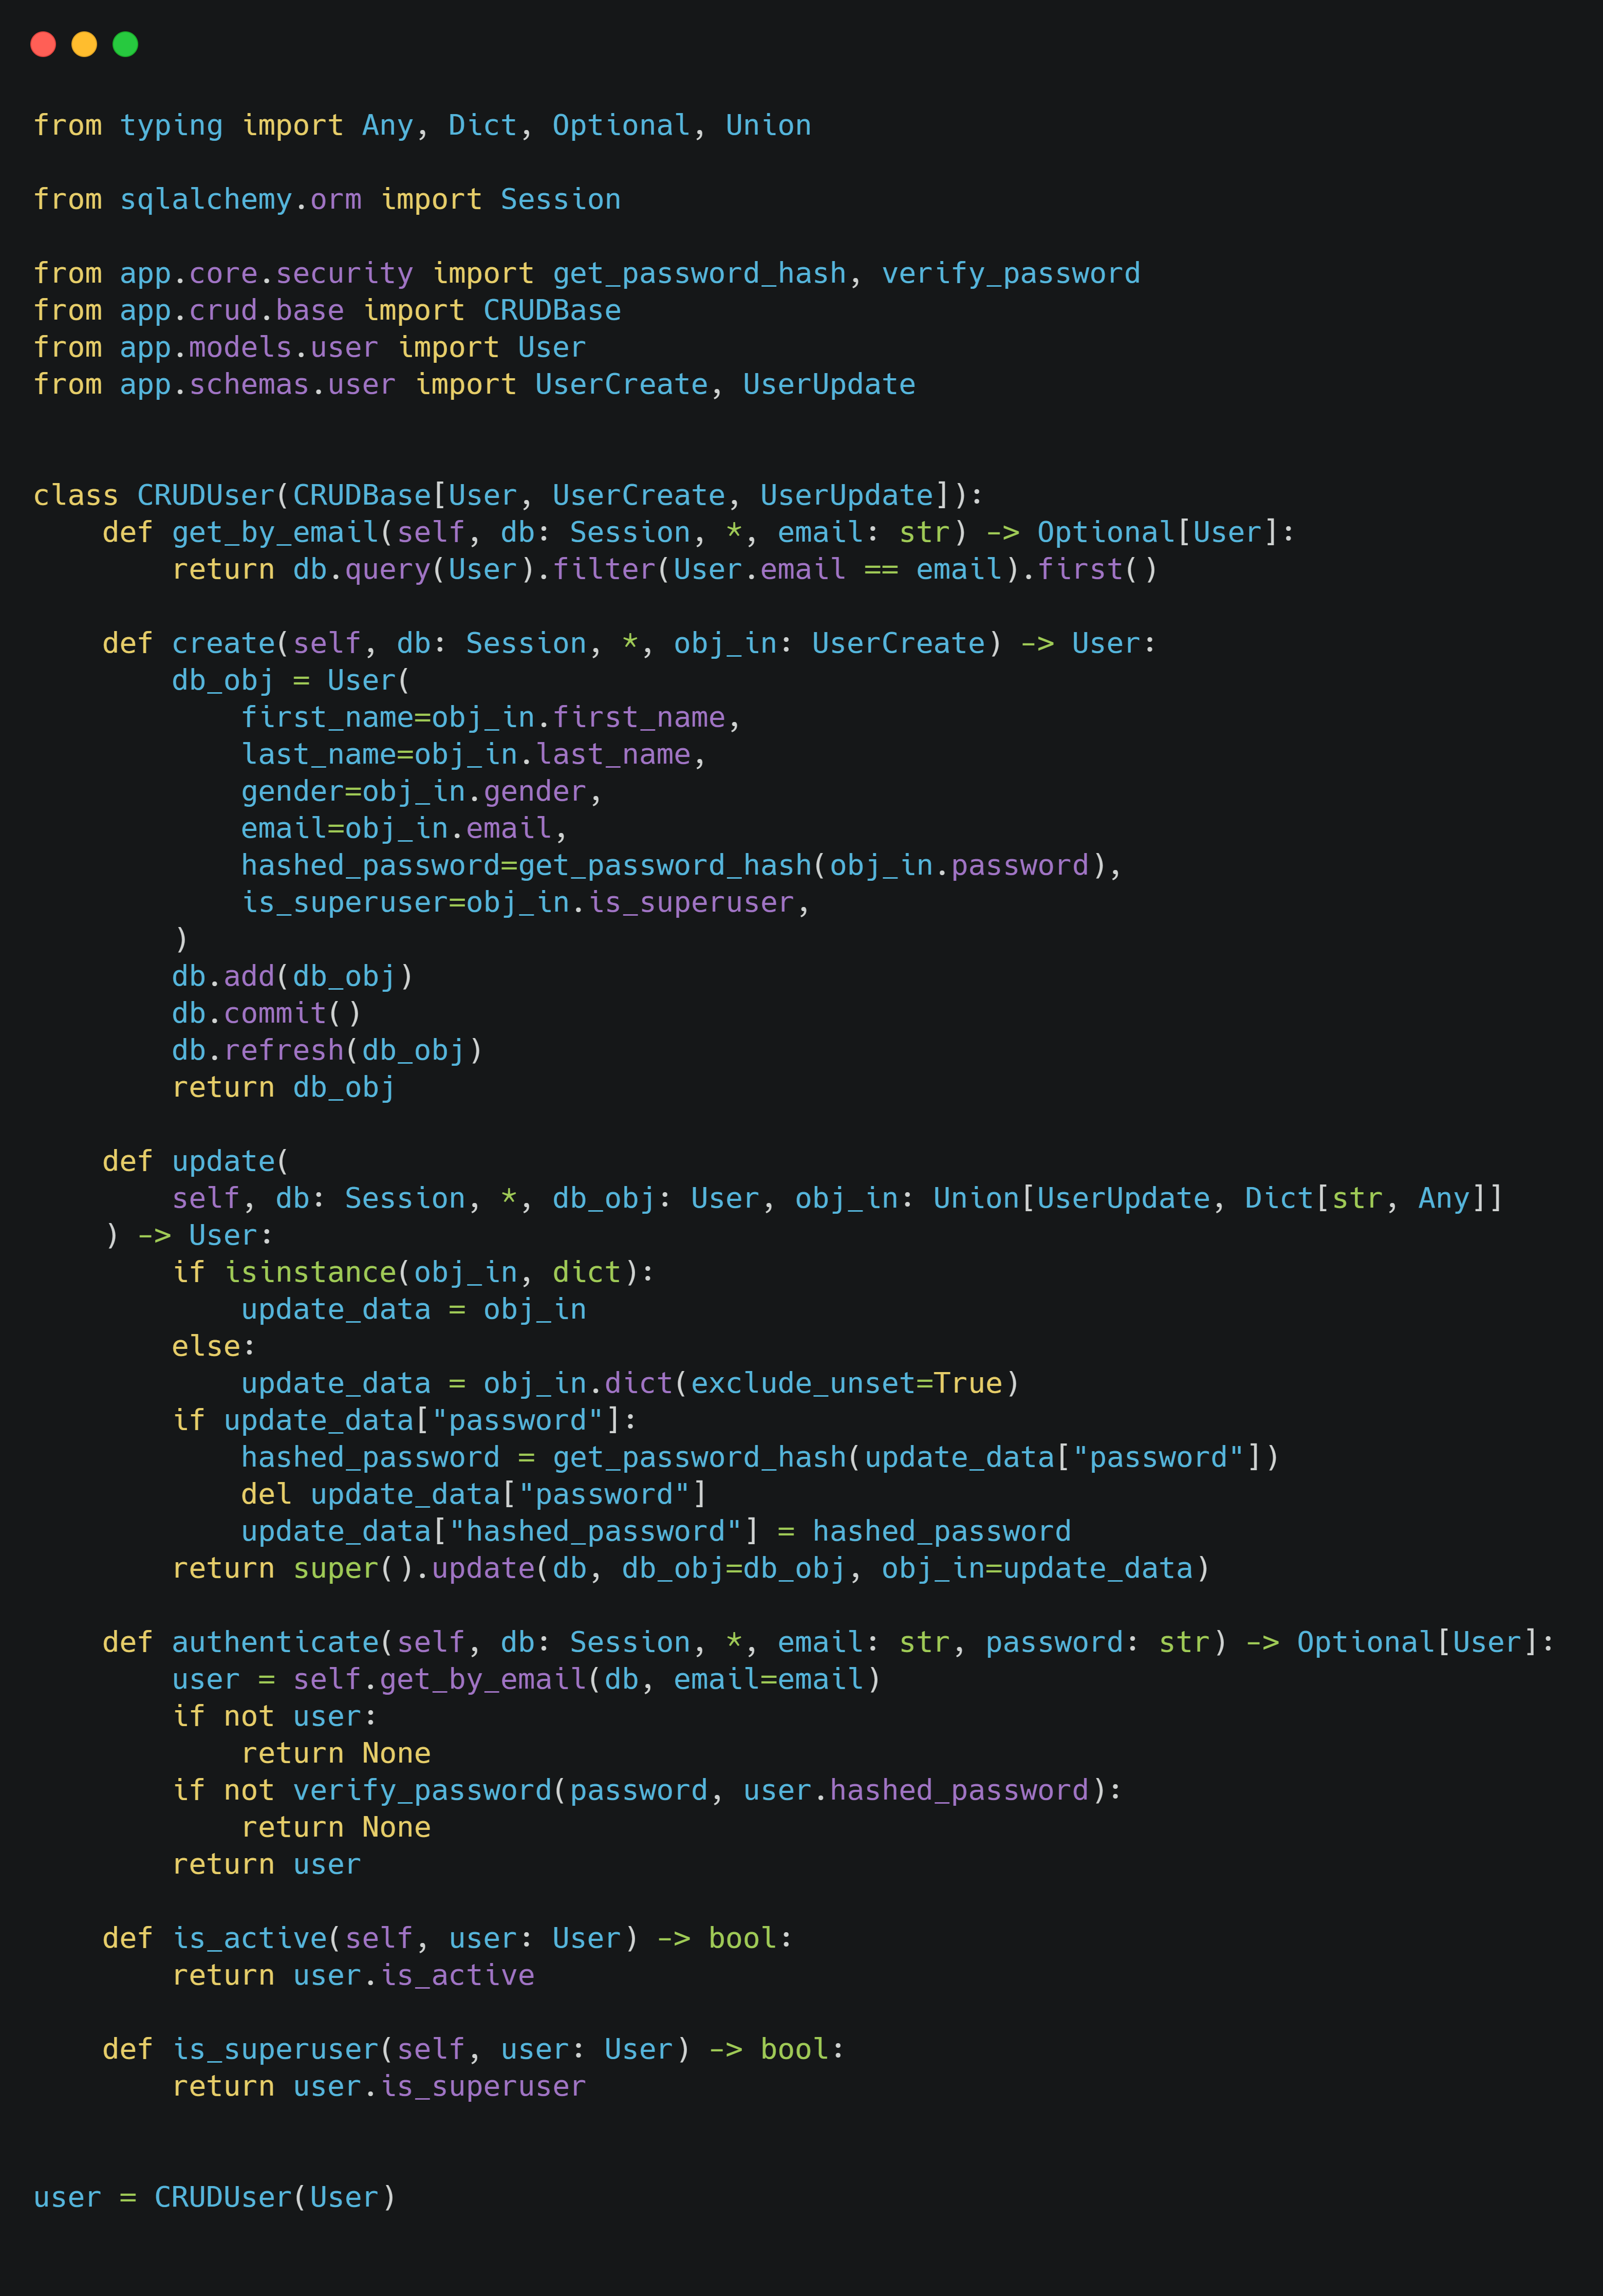
\includegraphics[scale=.10]{TT/img/implementacion/crud_user.png}
    \caption{CRUD de usuario}
    \label{graphic:user_crud}    
\end{figure}

Una de las carpetas esenciales es la llamada \textit{db}, en esta se encuentra la conexión con la base de datos y los archivos que gestiona el arranque de la base de datos, la conexión con el sistema gestor de la base de datos, en este caso postgres, los modelos que se usarán para la base de datos y que alembic y sqlalchemy necesitan para crear y modificar la base de datos en postgres, así como la creación del primer súper-usuario si se ejecuta el contenedor por primera vez.

Por otro lado, tenemos a la carpeta \textit{core}, aquí es donde se encuentran los archivos que se encargan de la seguridad y la configuración del servidor que se ejecutará en el contenedor, algunas de las funciones que se pueden encontrar en estos archivos son: la dirección que sigue del dominio para acceder a los endpoints de la API, el algoritmo de encriptación que en este caso es \textbf{HS256}, la llave de encriptación que es hexadecimal de 32 bits, la duración del token, verificar contraseñas o crear tokens, etc.

A continuación se describe la carpeta \textit{api}, dentro de esta carpeta se localizan los endpoints de la API y funciones importantes como se aprecia en la figura \ref{graphic:deps}, en donde se aprecia las funciones para obtener estados del usuario que son necesarios para validar las peticiones que se harán a la base de datos. En los archivos que se pueden encontrar dentro de esta carpeta, están los responsables de realizar las peticiones HTTP a la base de datos \textit{(Get, Put, Post, Delete)}. En las figuras \ref{graphic:user_endpoint_1} y \ref{graphic:user_endpoint_2} se detallan todas las funciones para las peticiones HTTP que corresponden al usuario, también se pueden definir los estados de error en caso de que la petición que se realice falle.

\begin{figure}[!htb]
    \centering
    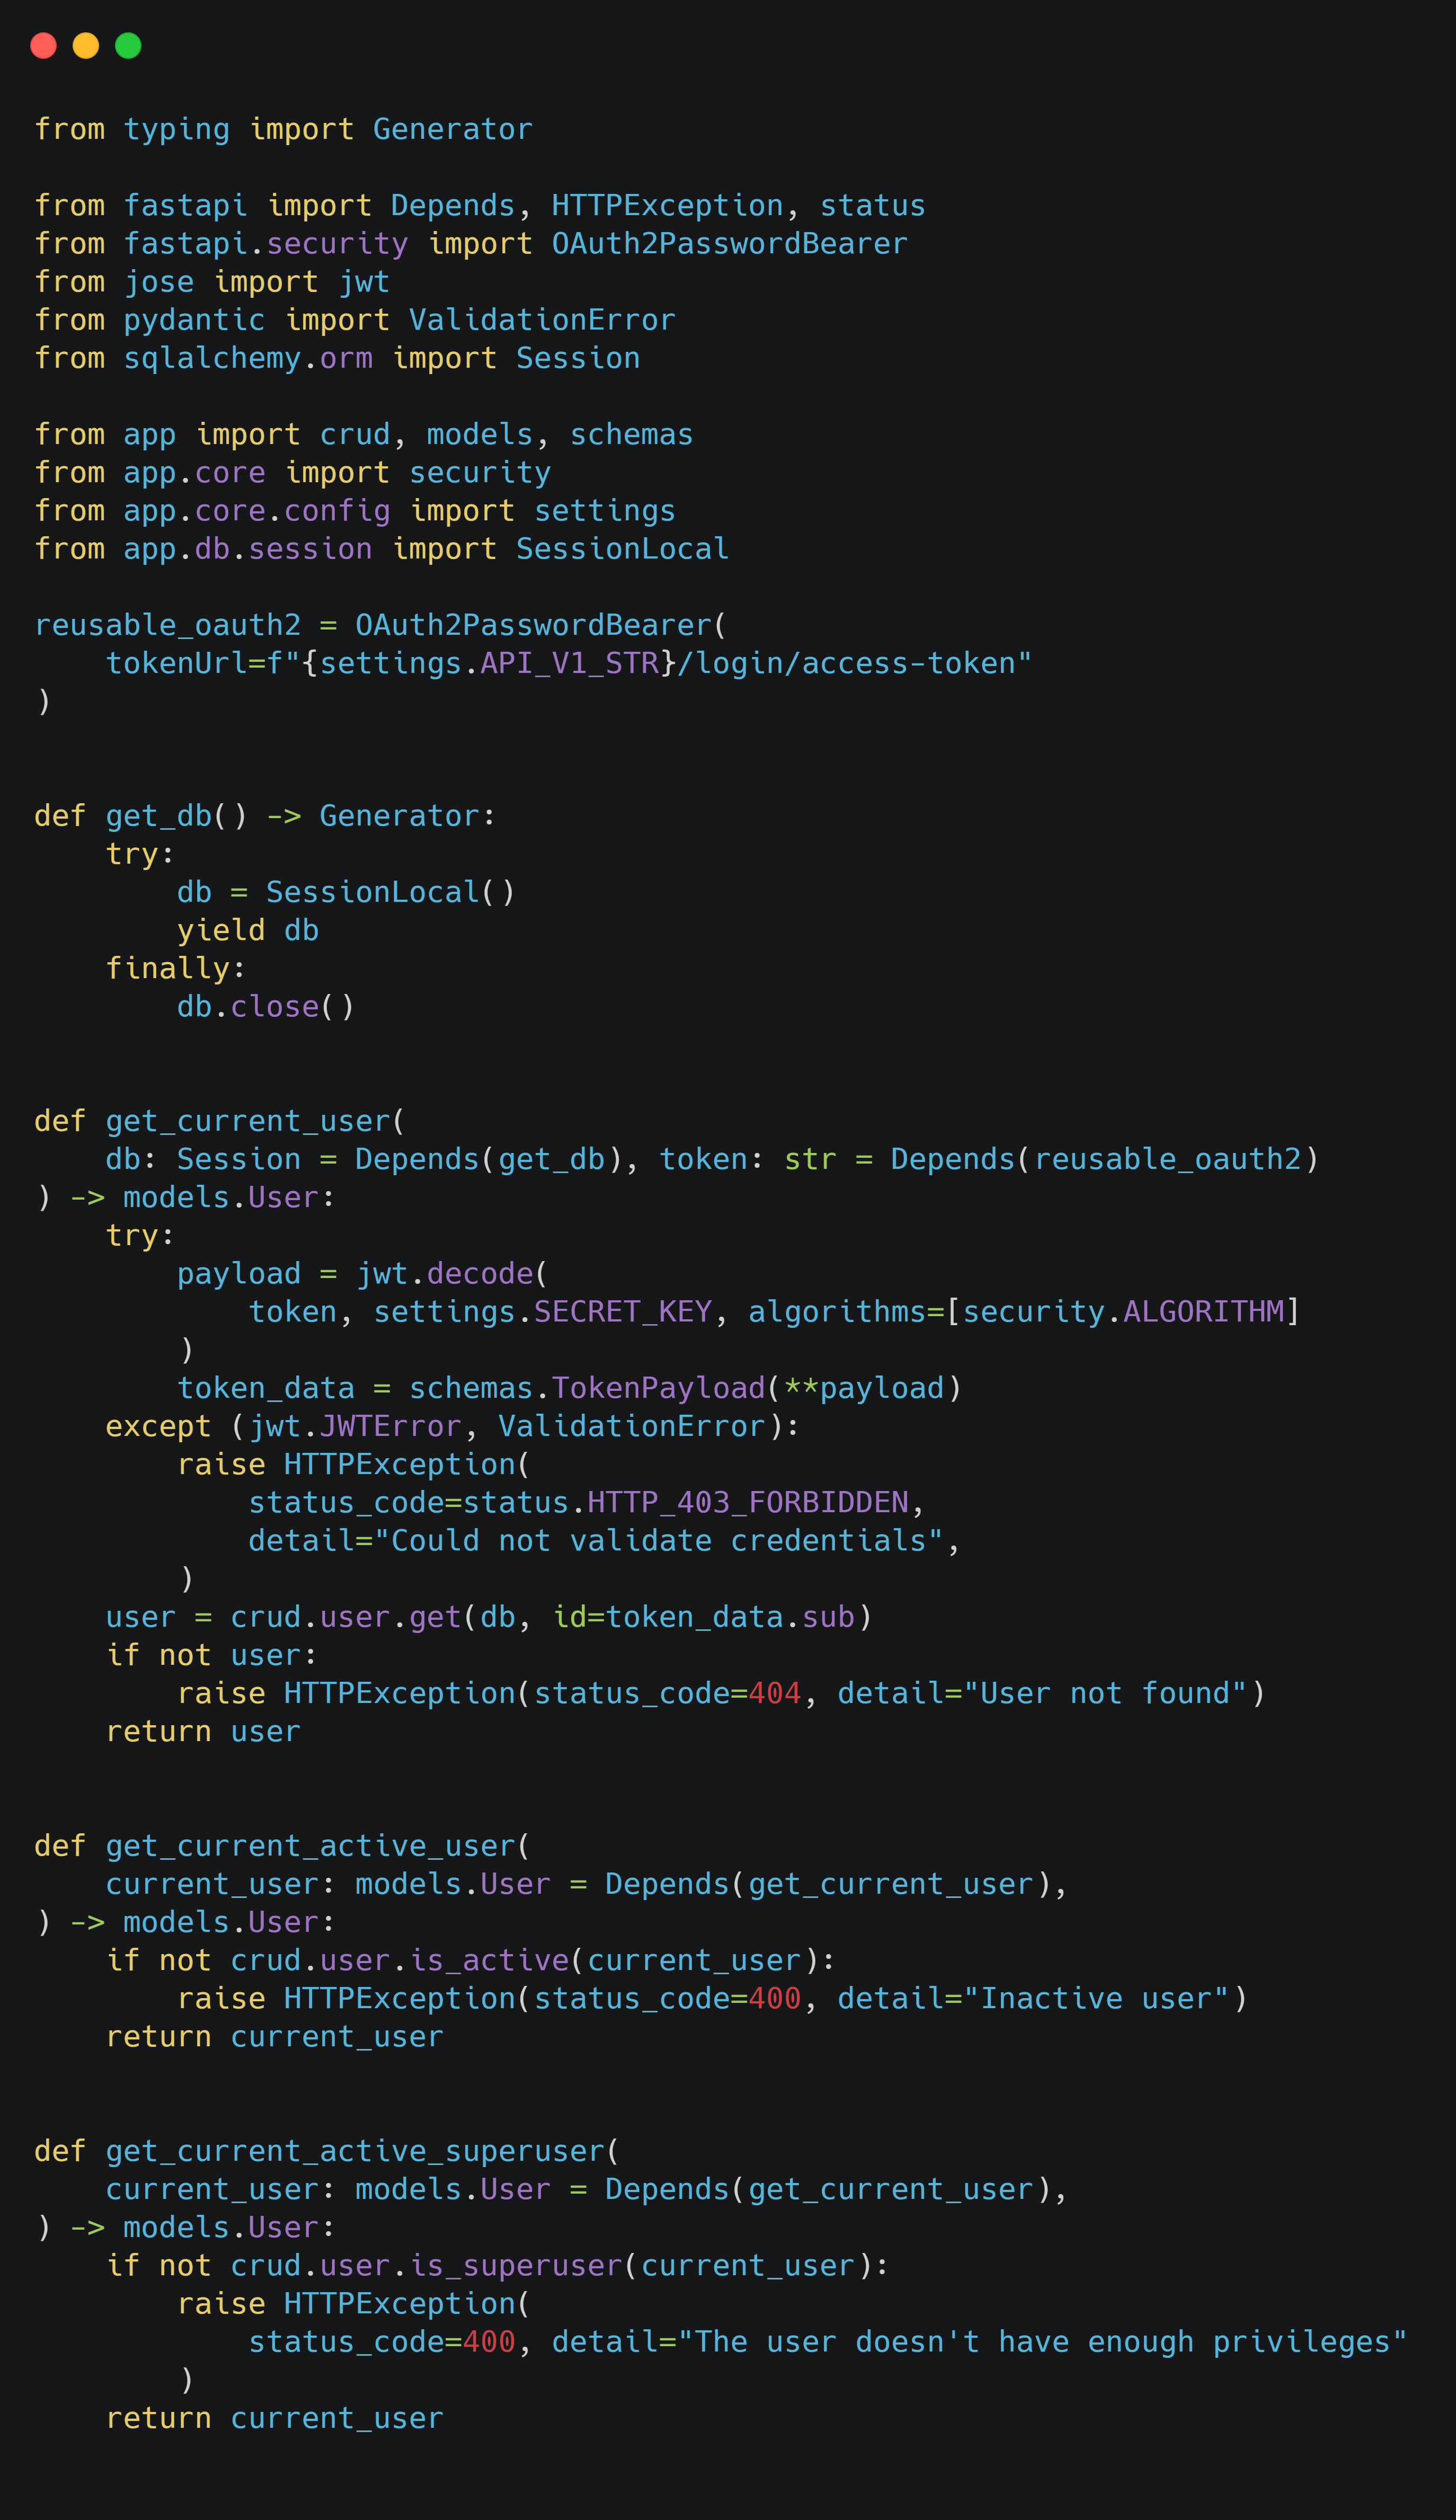
\includegraphics[scale=.10]{TT/img/implementacion/deps.png}
    \caption{Funciones para obtener estados del usuario}
    \label{graphic:deps}    
\end{figure}

\begin{figure}[!htb]
    \centering
    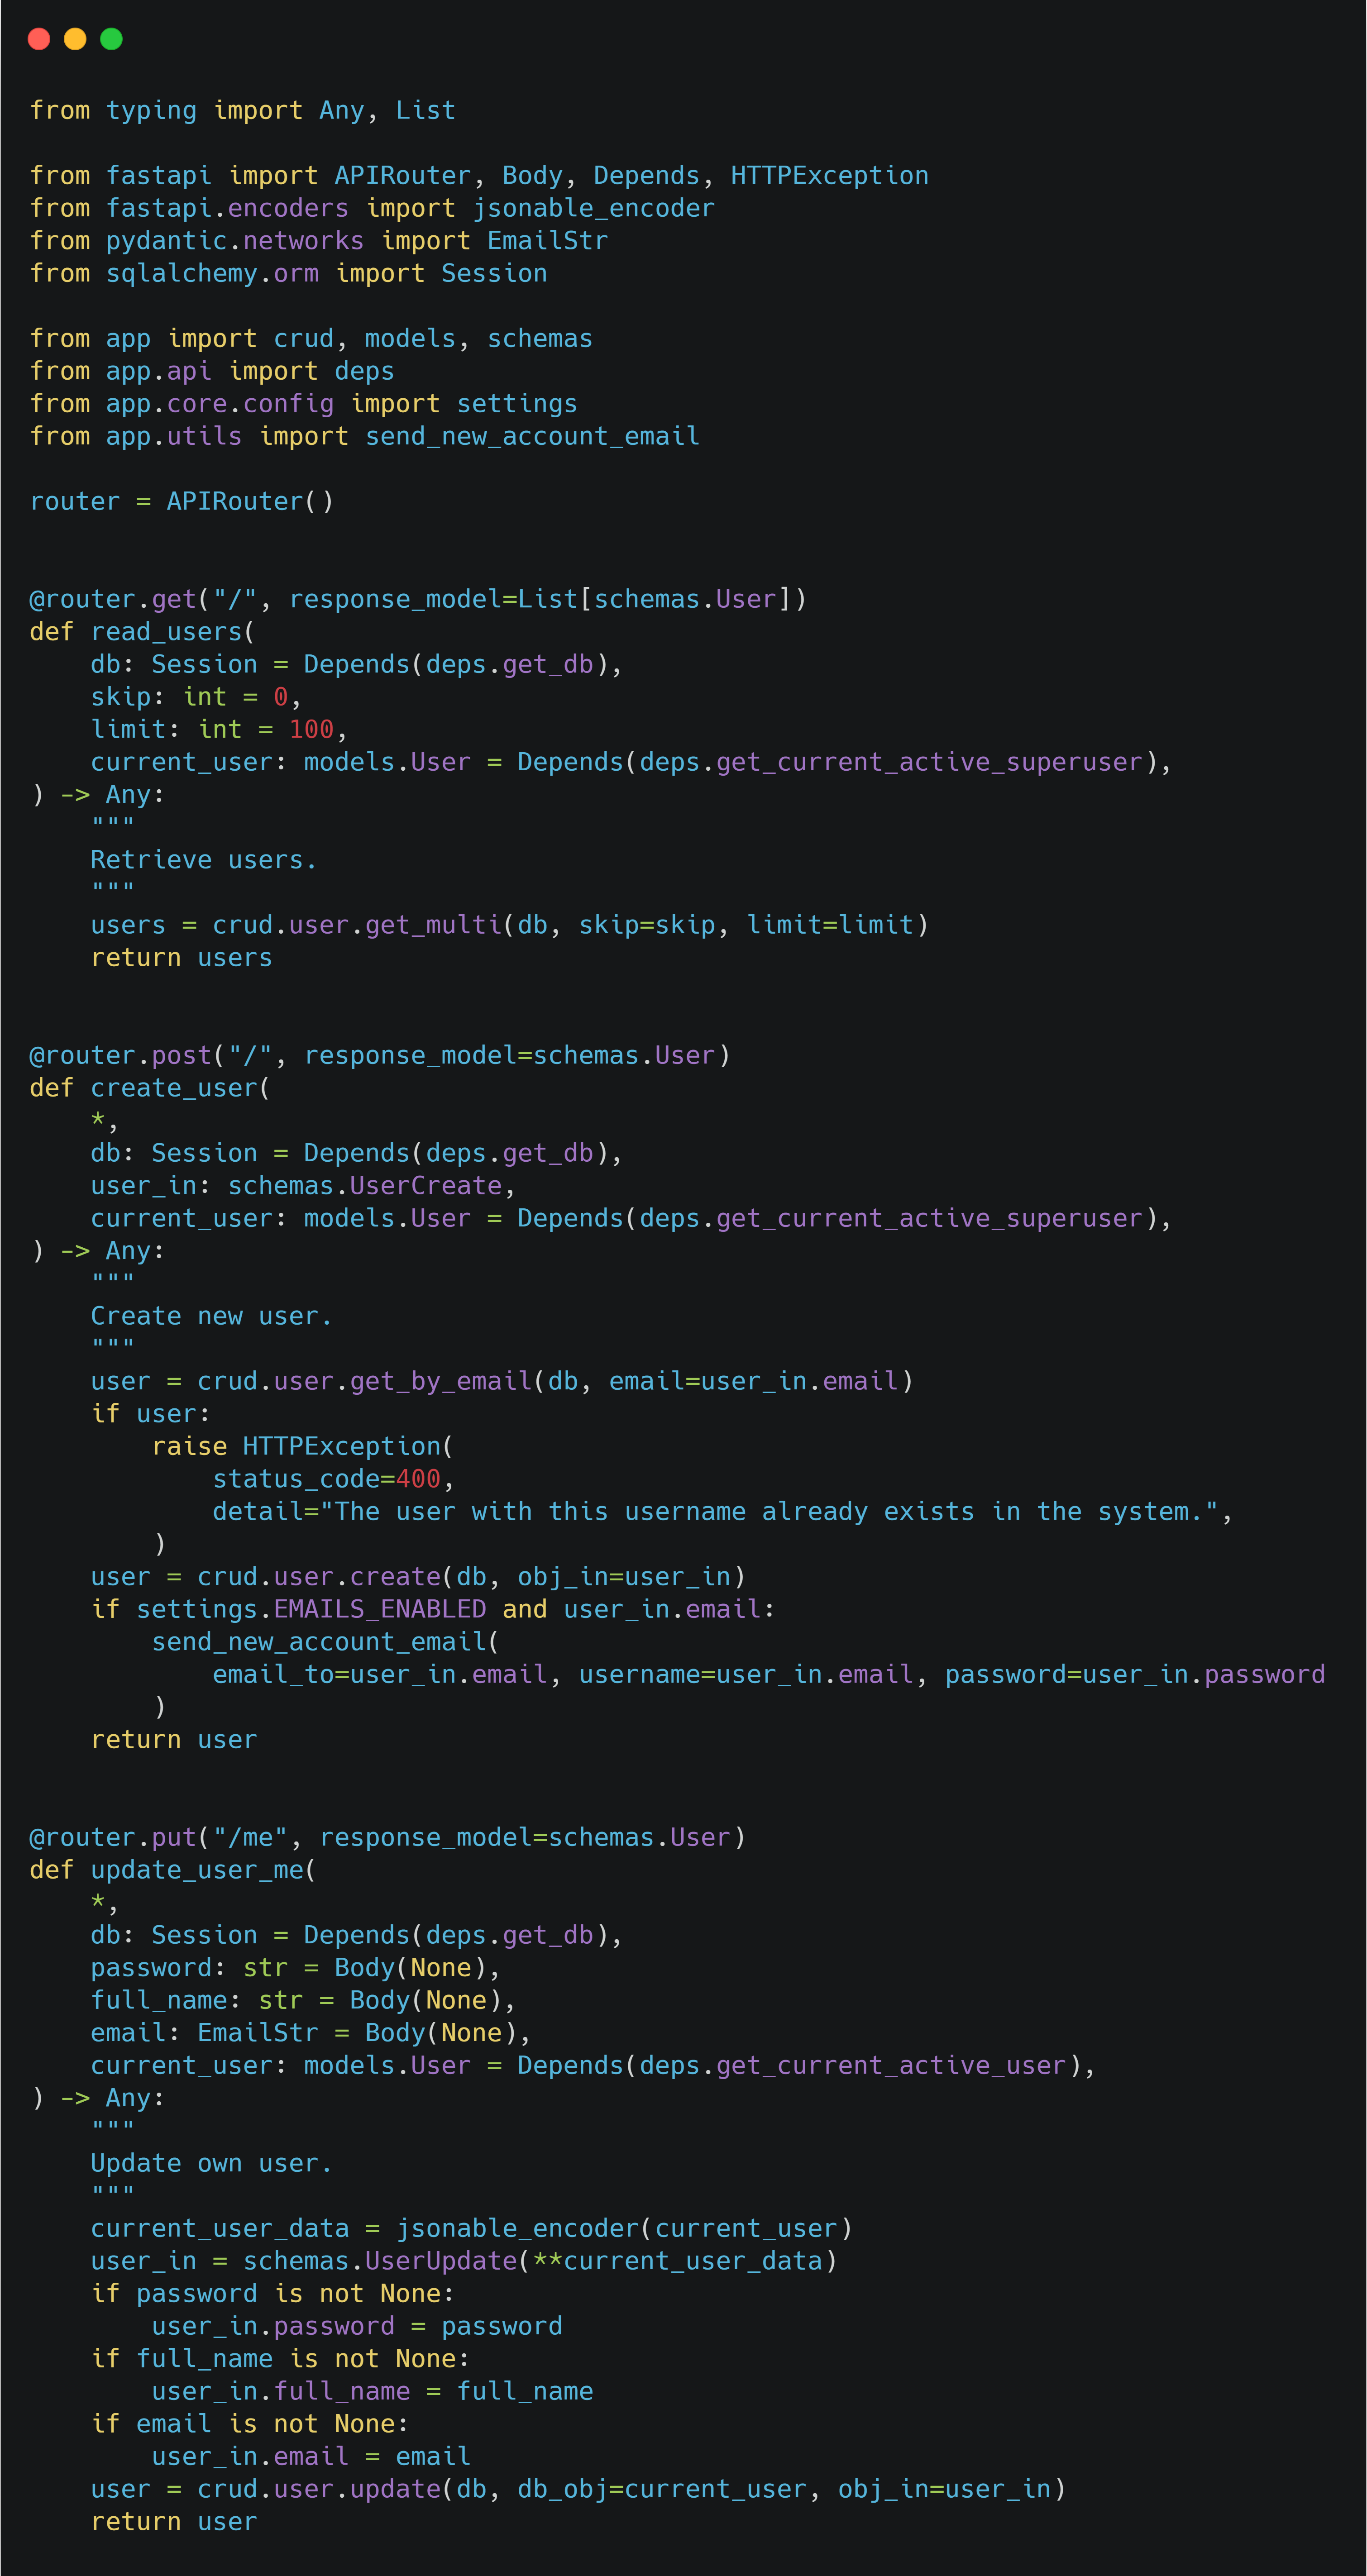
\includegraphics[scale=.10]{TT/img/implementacion/user_endpoint_1.png}
    \caption{Funciones para realizar peticiones de la API - Parte 1}
    \label{graphic:user_endpoint_1}    
\end{figure}

\begin{figure}[!htb]
    \centering
    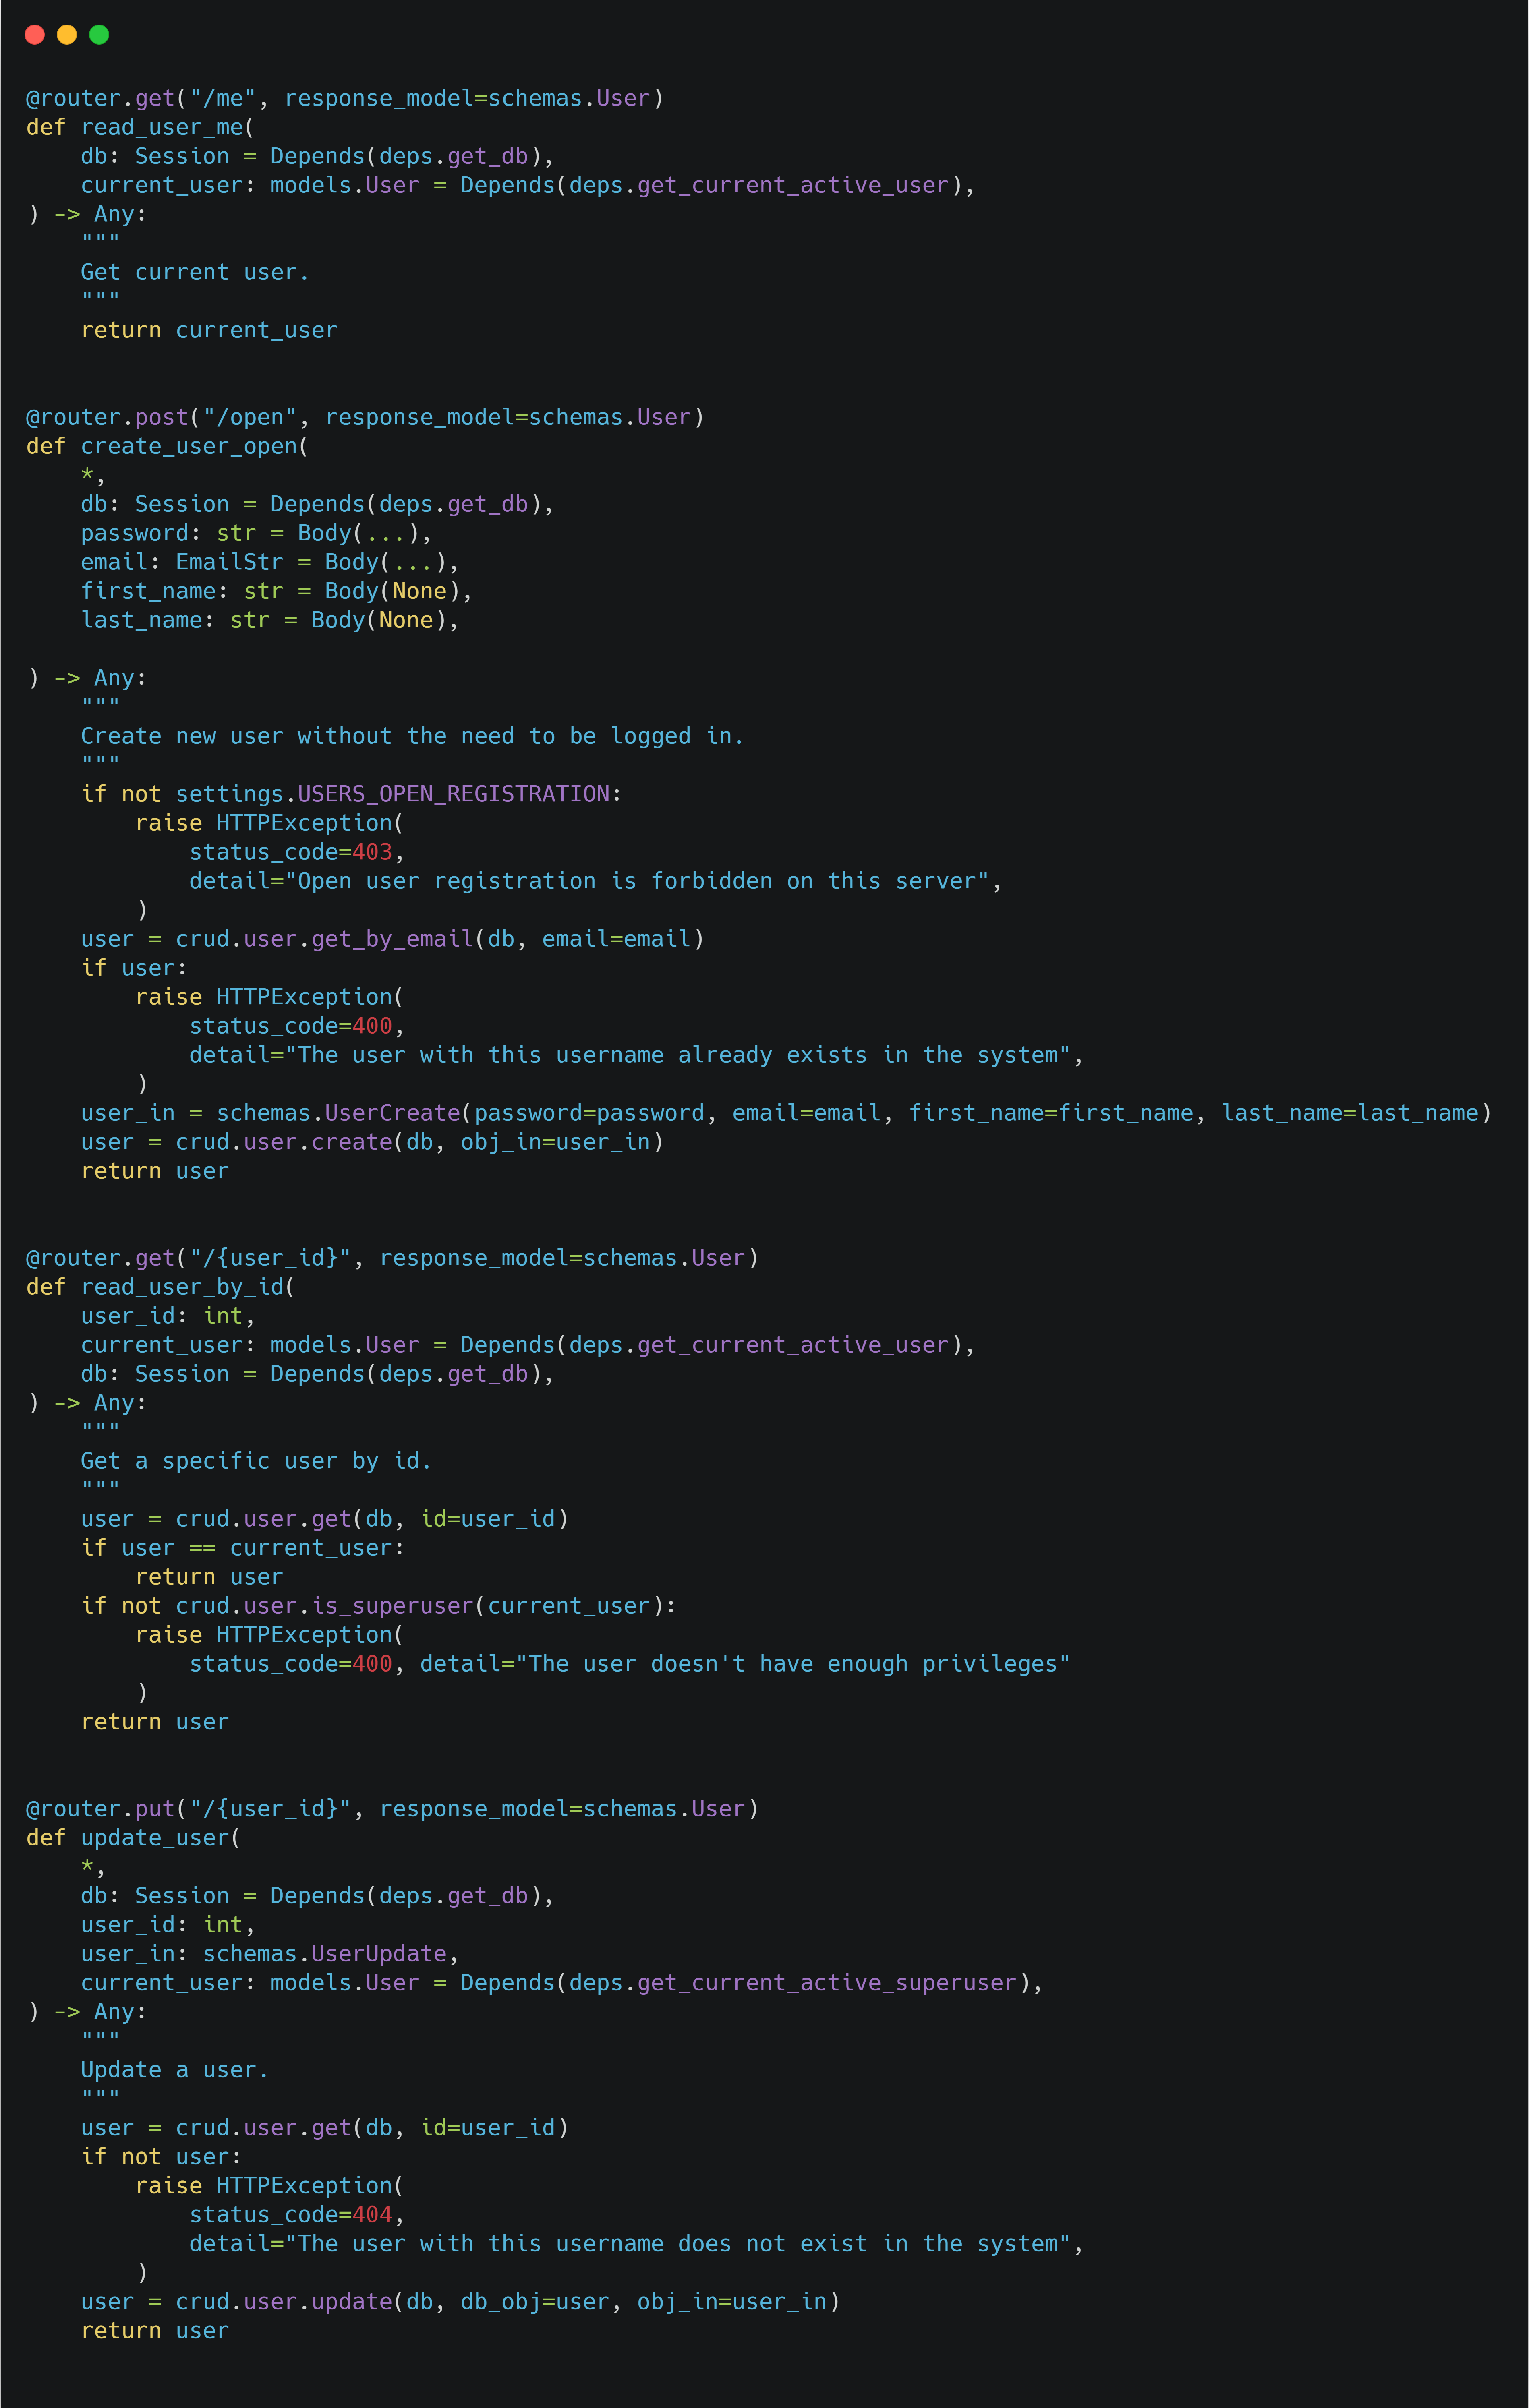
\includegraphics[scale=.10]{TT/img/implementacion/user_endpoint_2.png}
    \caption{Funciones para realizar peticiones de la API - Parte 2}
    \label{graphic:user_endpoint_2}    
\end{figure}

Para finalizar esta sección se describirán las carpetas y archivos faltantes. Primero, describimos la carpeta \textit{email-templates}, en esta carpeta se encuentran los archivos que tienen el diseño para enviar correos electrónicos para la creación de cuenta nueva, restablecer la contraseña y un template de prueba. En segundo lugar, la carpeta \textit{tests} almacena los archivos para realizar pruebas de funcionamiento a la API. Por último, pero no menos importante, los archivos que están en app, la mayoría de estos han sido creados para poder ejecutar la API en la imagen del contenedor de python, así como inicializar las pruebas a la API y archivos que tienen funciones variadas para las pruebas o para realizar cálculos que son necesarios para las predicciones del sistema.

\clearpage
\subsubsection{Oauth2}
En las secciones anteriores se ha hablado un poco de la seguridad del sistema con el uso de token y la generación de una llave del sistema basada en el algoritmo HS256, con ello podemos abordar el manejo del acceso a los endpoints del sistema, para esto se ha usado un protocolo de autorización que viene integrado en FastApi, hablamos del protocolo de autorización OAuth2. Este es un estándar abierto para las API's consiste en compartir información entre sitios sin tener que compartir la identidad.

Oauth surge para paliar la necesidad que se establece del envío continuo de credenciales entre cliente y servidor. También facilita la integración de terceros como Facebook, Google O Twitter, con esto no es necesario almacenar las credenciales de esas aplicaciones, con ello se pueden realizar las acciones que desee a su nombre.

En el sistema, Oauth2 se ha usado para blindar algunos endpoints, esto se refiere a que no va a ser posible acceder a esos recursos sin antes haber iniciado sesión y tener un token válido. Como el sistema va a ser consumido por una aplicación web, este se define como cliente público el cual no puede mantener contraseñas a salvo, por ende, para realizar la autenticación se ha usado el tipo de otorgamiento que consiste en que el usuario ingrese sus credenciales (correo y contraseña) para la obtención del token de acceso, recordando que este tiene un tiempo de expiración, dando como resultado el acceso a los recursos que estaban bloqueados.

\subsubsection{Documentación de FastApi - 'docs'}
Una de las ventajas por las que se ha elegido desarrollar basándose en Python con ayuda del Framework FastApi, es que al momento de ir desarrollando los endpoint de la API se genera de manera automática la documentación de todos estos, teniendo como resultado dos versiones de paginas web que se pueden consultar al momento de inicializar el contenedor, en esta sección mostraremos la documentación con la cual se pueden hacer pruebas, esta enfocada en la realización de pruebas manualmente, en la figura \ref{graphic:docs1} se puede apreciar la documentación generada por fastapi. En esa página web aparecerán todos los endpoints que se ha desarrollado para el sistema y al final, los esquemas que se han creado para realizar las peticiones necesarias del sistema. Un detalle a destacar es el icono del candado, aquellos endpoints que requieran una autorización del sistema, tendrán un icono de un candado en color gris, esto es porque no se tiene la autorización necesaria y será necesario iniciar sesión.

\begin{figure}[!htb]
    \centering
    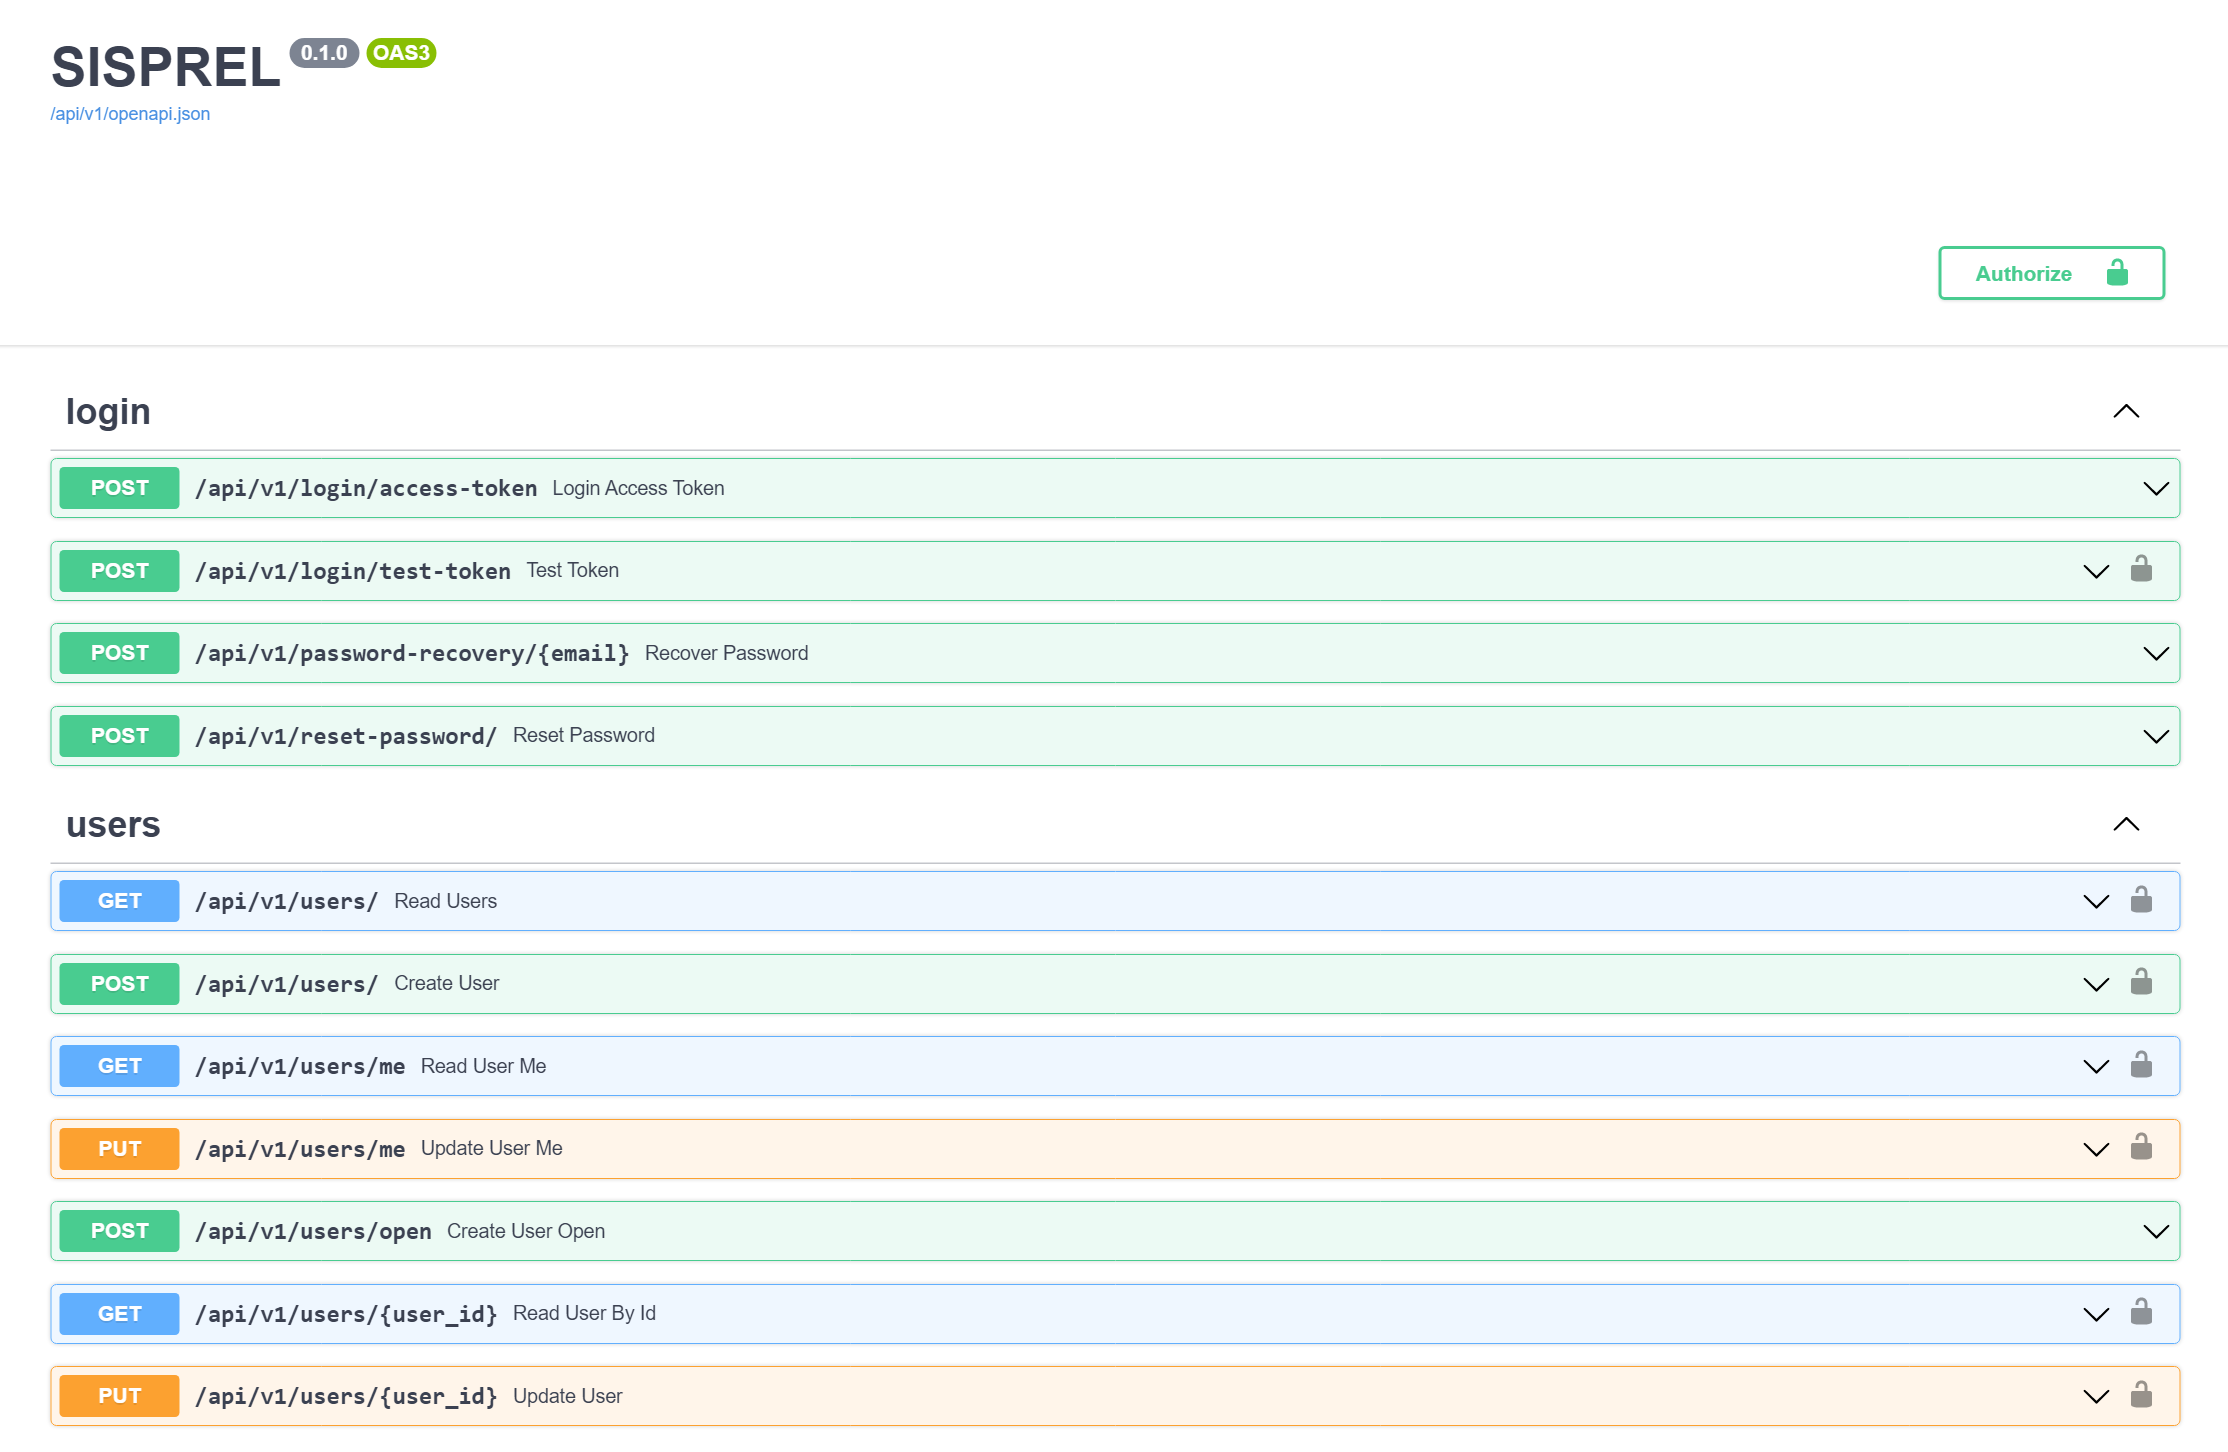
\includegraphics[scale=.20]{TT/img/implementacion/docs_1.png}
    \caption{Documentación 'docs' - Parte 1}
    \label{graphic:docs1}    
\end{figure}

Como se ha descrito anteriormente, esta versión de la documentación permite realizar pruebas, por lo tanto, para tener acceso a los endpoint que estan bloqueados, procedemos a iniciar sesión, en la imagen \ref{graphic:docs1} se puede observar un botón llamado Authorize, al darle clic nos mostrará un aviso como se puede apreciar en la imagen \ref{graphic:docs2} en donde nos pide algunos datos, los únicos que se van a requerir para acceder al sistema, ya sea con el uso de esta documentación o en cualquier aplicación que la consuma, es requerido ingresar el "username" que es el correo electrónico y la contraseña. Al ingresarlos y que sean correctos, nos sale otro aviso de que ha sido aprobada nuestra autorización  como se aprecia en la imagen \ref{graphic:docs3} y se nos otorga un token, el cual nos dará acceso a los endpoints del sistema y nos permite realizar las peticiones que estén disponibles.

\begin{figure}[!htb]
    \centering
    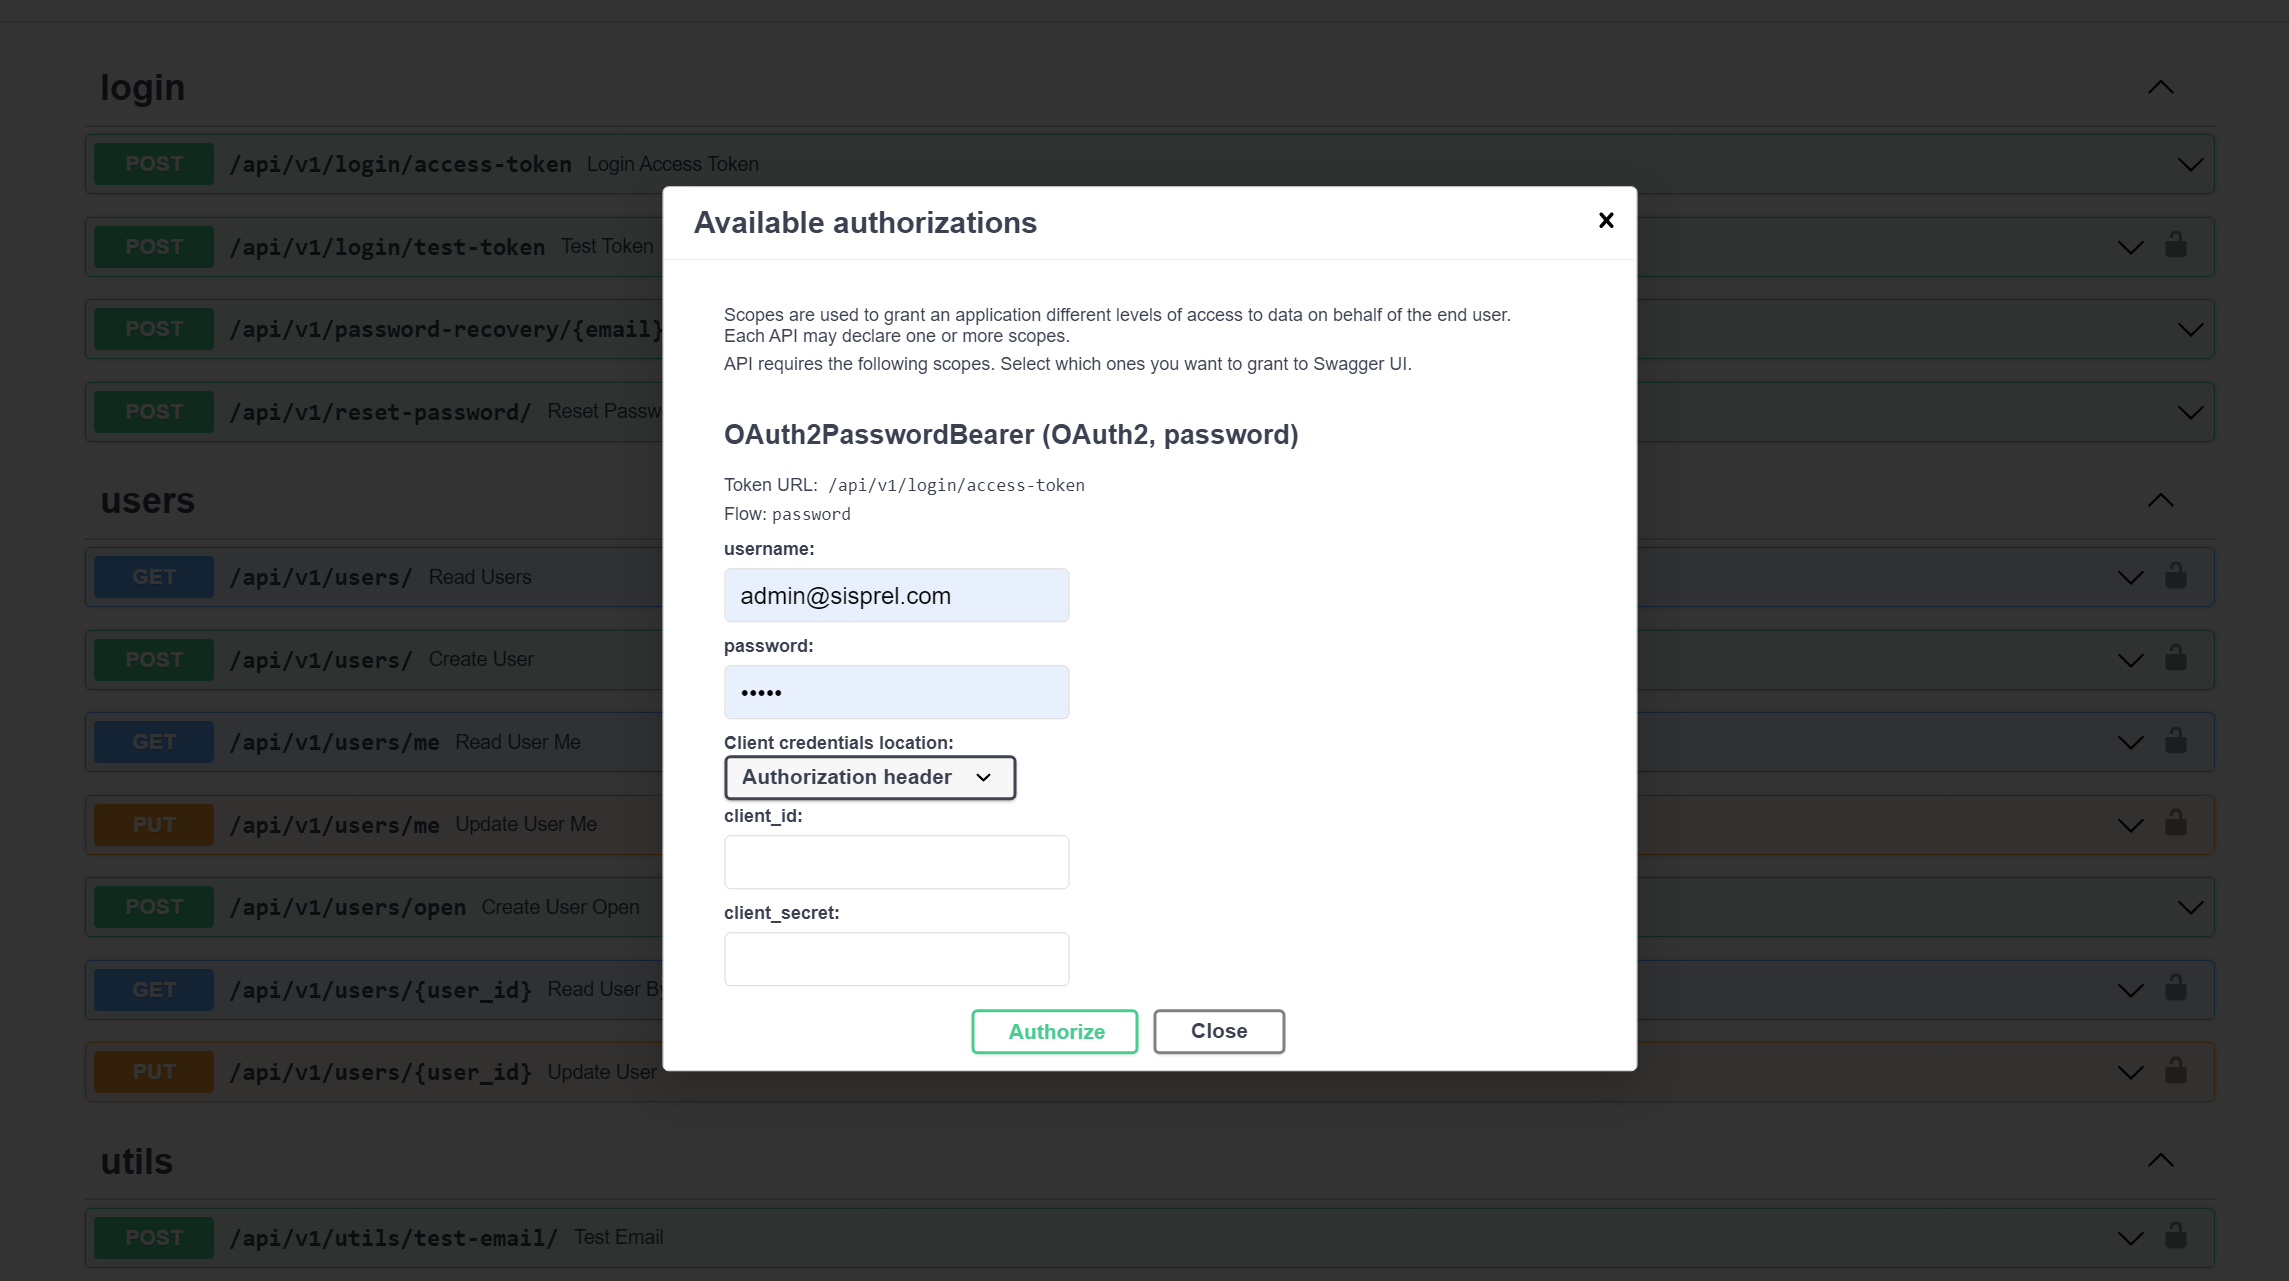
\includegraphics[scale=.20]{TT/img/implementacion/docs_2.png}
    \caption{Documentación 'docs' - Parte 2}
    \label{graphic:docs2}    
\end{figure}

\begin{figure}[!htb]
    \centering
    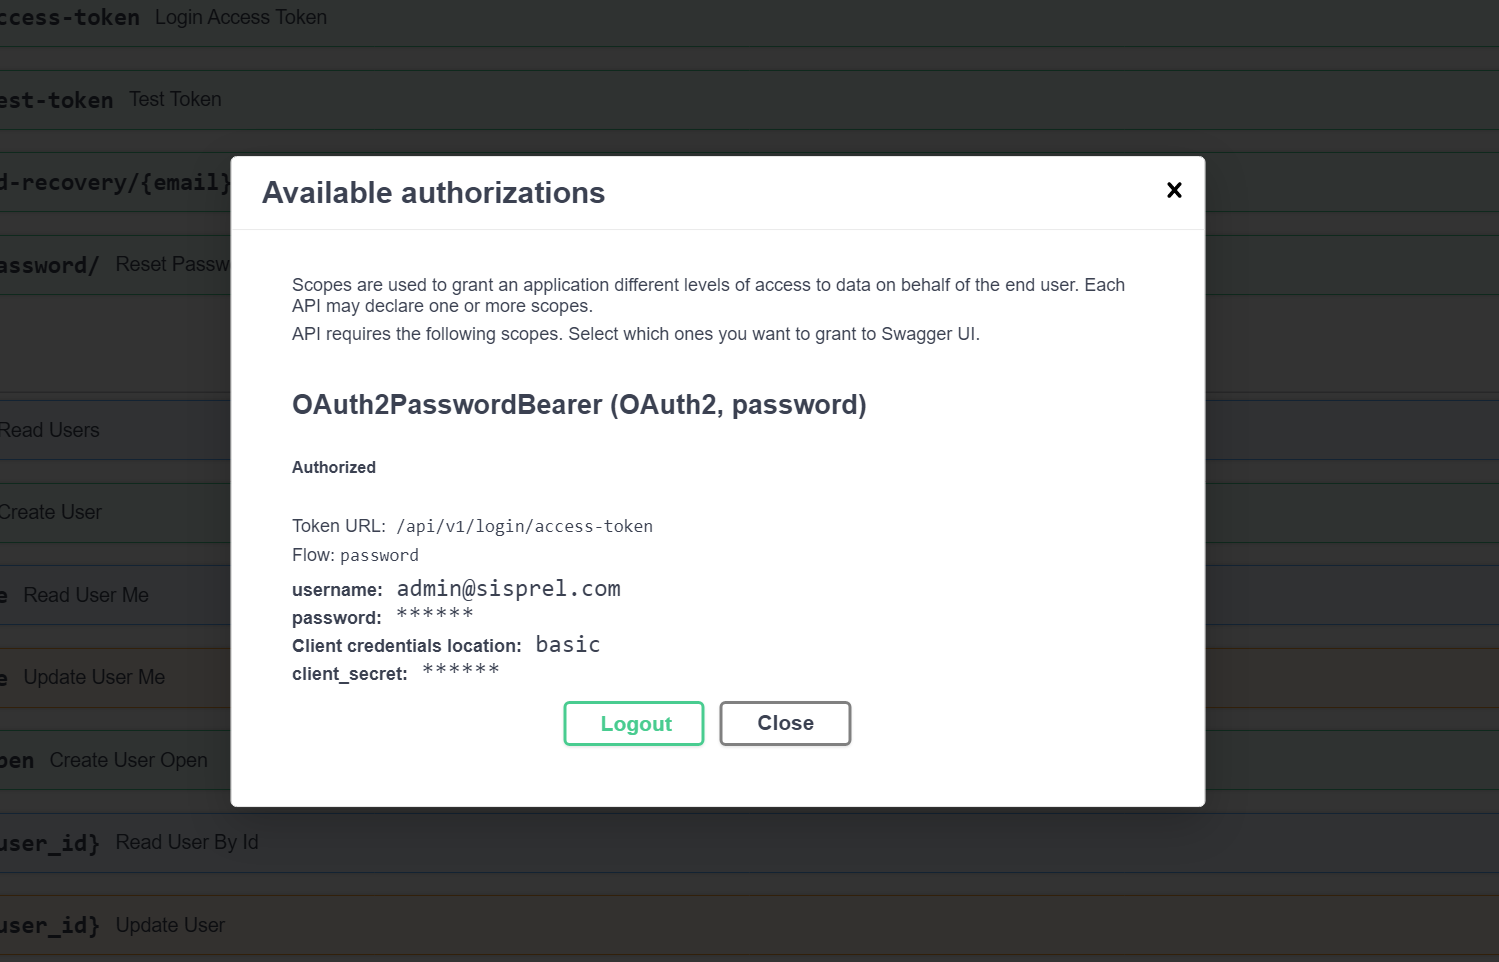
\includegraphics[scale=.30]{TT/img/implementacion/docs_3.png}
    \caption{Documentación 'docs' - Parte 3}
    \label{graphic:docs3}
\end{figure}

Teniendo el token de acceso, podemos realizar pruebas en los endpoints blindados, pero sin el, también podemos probar endpoints pero solo los que no están blindados. En la figura \ref{graphic:docs4} se muestra la interfaz del endpoint, al seleccionarlo nos muestra que datos hay que enviar y como va a devolver la respuesta la API, un código 200 significa que la petición ha sido cumplida y nos devuelve lo que hemos creado o pedido, un error 422 es un error de validación, ya sea porque se mandó algo mal o que no respeta el tipo de dato que se requiere y un error 402 es porque no tenemos autorización a ese recurso.

\begin{figure}[!htb]
    \centering
    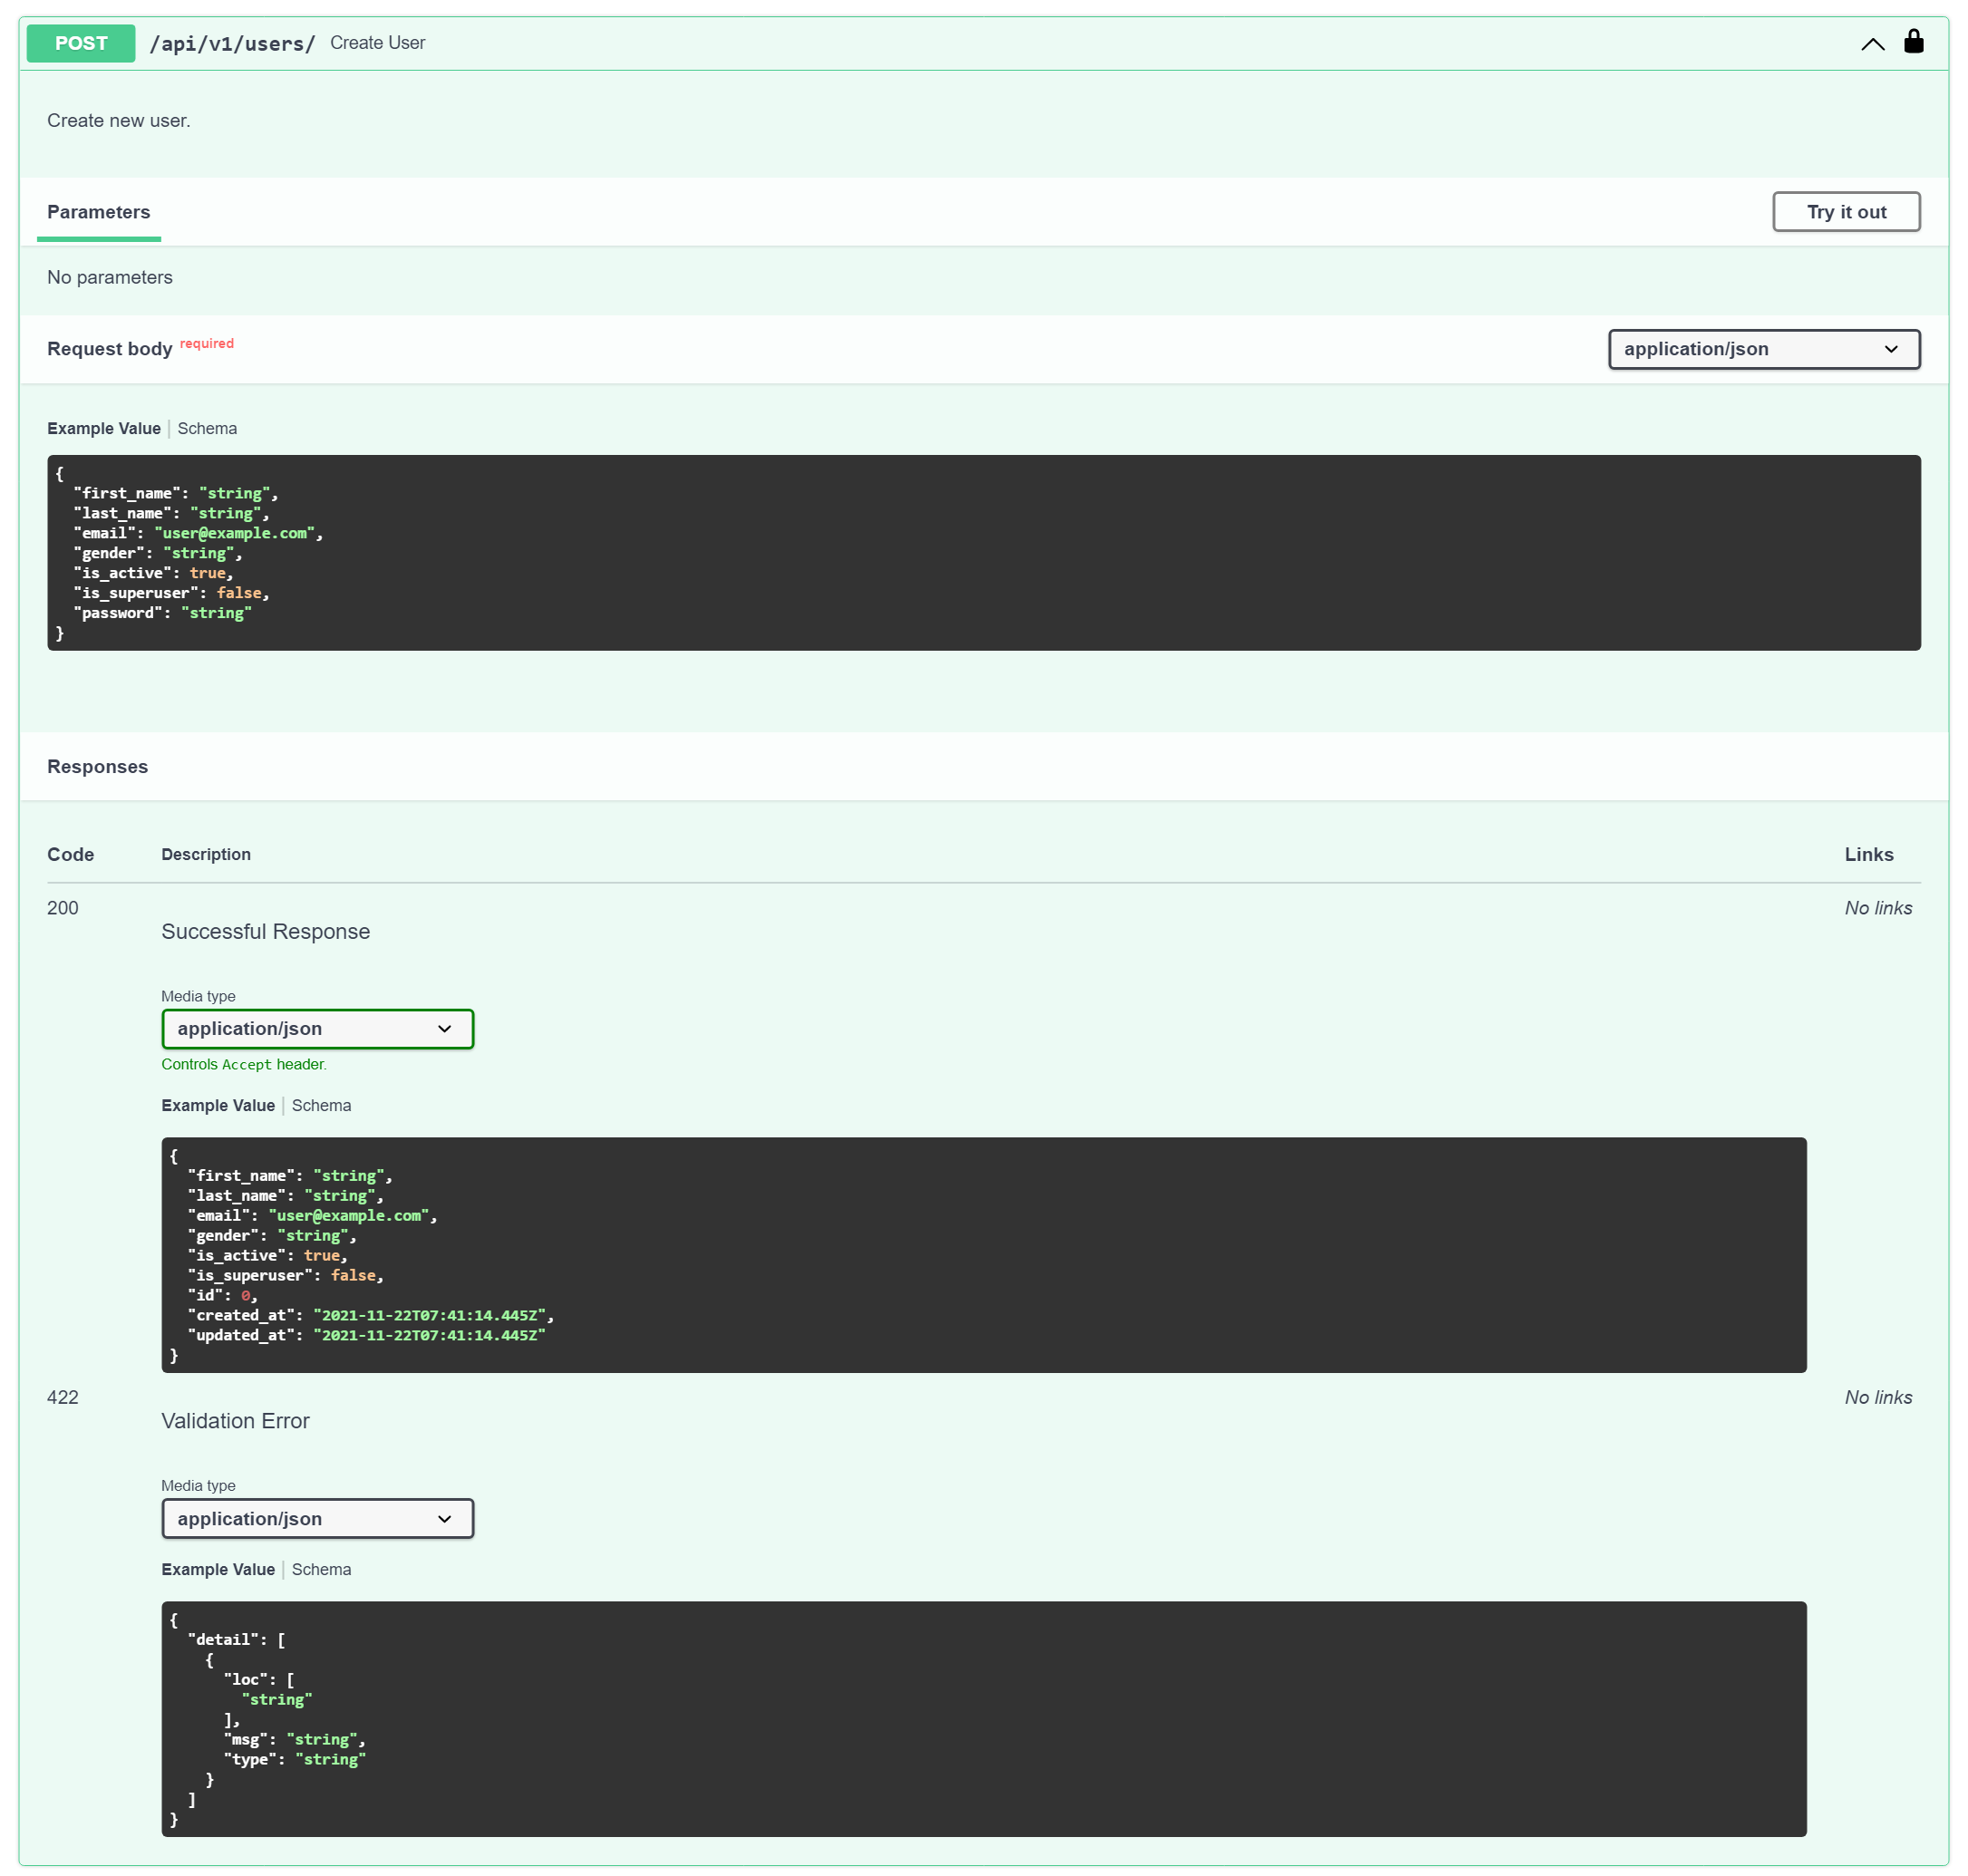
\includegraphics[scale=.20]{TT/img/implementacion/docs_4.png}
    \caption{Documentación 'docs' - Parte 4}
    \label{graphic:docs4}
\end{figure}

Como se mencionó en el parrafo anterior, se pueden realizar pruebas a la API desde esta página, lo que nos evita usar software de terceros para realizarlas tal como lo es por ejemplo Postman, para acceder a ello le damos clic al boton 'Try it out' nos habilitará una sección para mandar un JSON en el caso de realizar un POST a la API, un ID para la consulta o la eliminación de un objeto en la base de datos, en el caso de la imagen \ref{graphic:docs5} se presenta el caso para crear un usuario, por lo tanto se habilitarán los campos en formato JSON y el tipo de dato que este tiene que tener, se tiene que respetar el nombre del campo y se modifican los campos que se desea cambiar y  con ello, le damos clic al botón 'Execute' para ejecutar la petición y nos regresará el código y resultado correspondiente.

\begin{figure}[!htb]
    \centering
    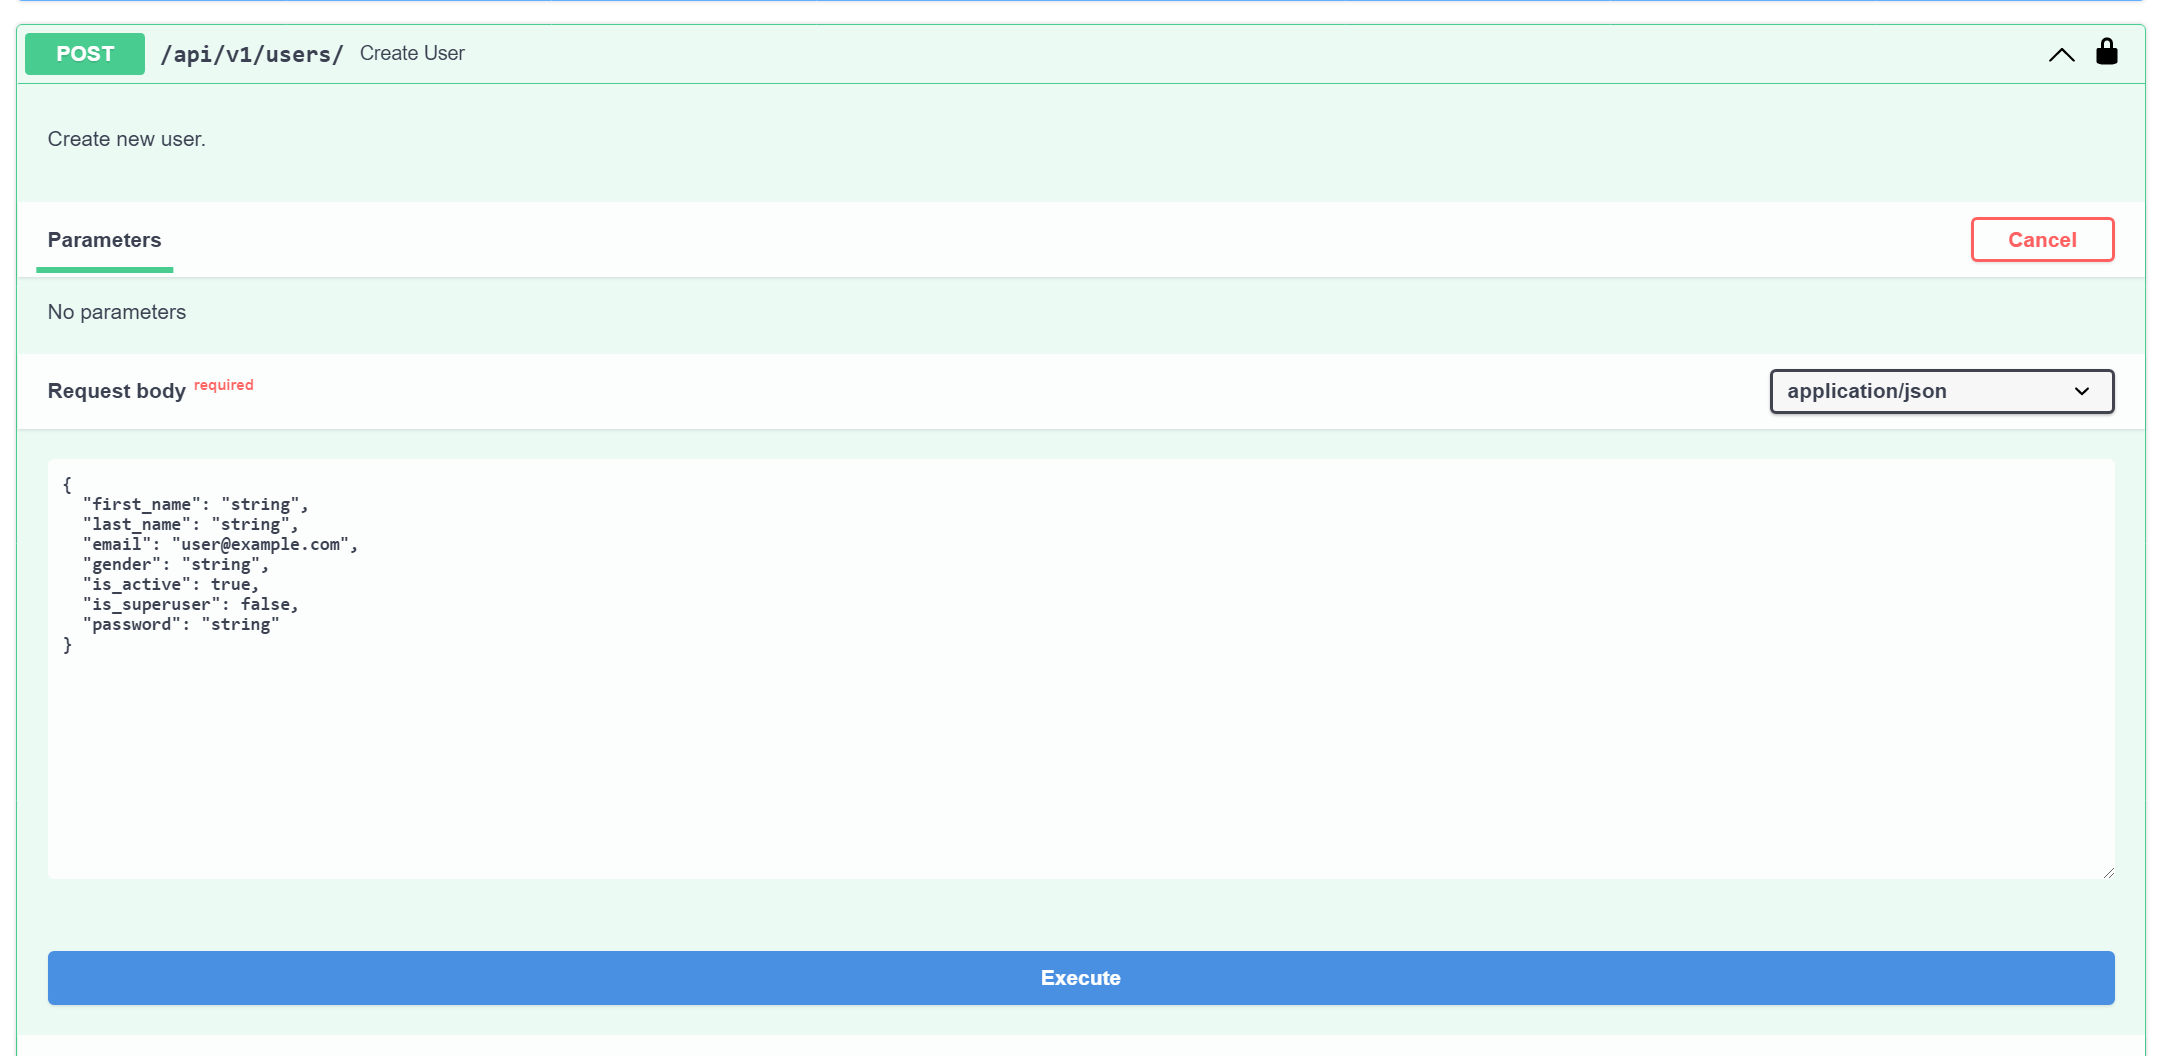
\includegraphics[scale=.20]{TT/img/implementacion/docs_5.png}
    \caption{Documentación 'docs' - Parte 5}
    \label{graphic:docs5}
\end{figure}

Por último, esta versión de la documentación nos genera la lista de los esquemas usados por la API mostrados en la imagen \ref{graphic:docs6}, estos contienen el nombre del esquema y que es lo que pueden recibir o devuelven en formato JSON de acuerdo al tipo de petición que se realice.
\begin{figure}[!htb]
    \centering
    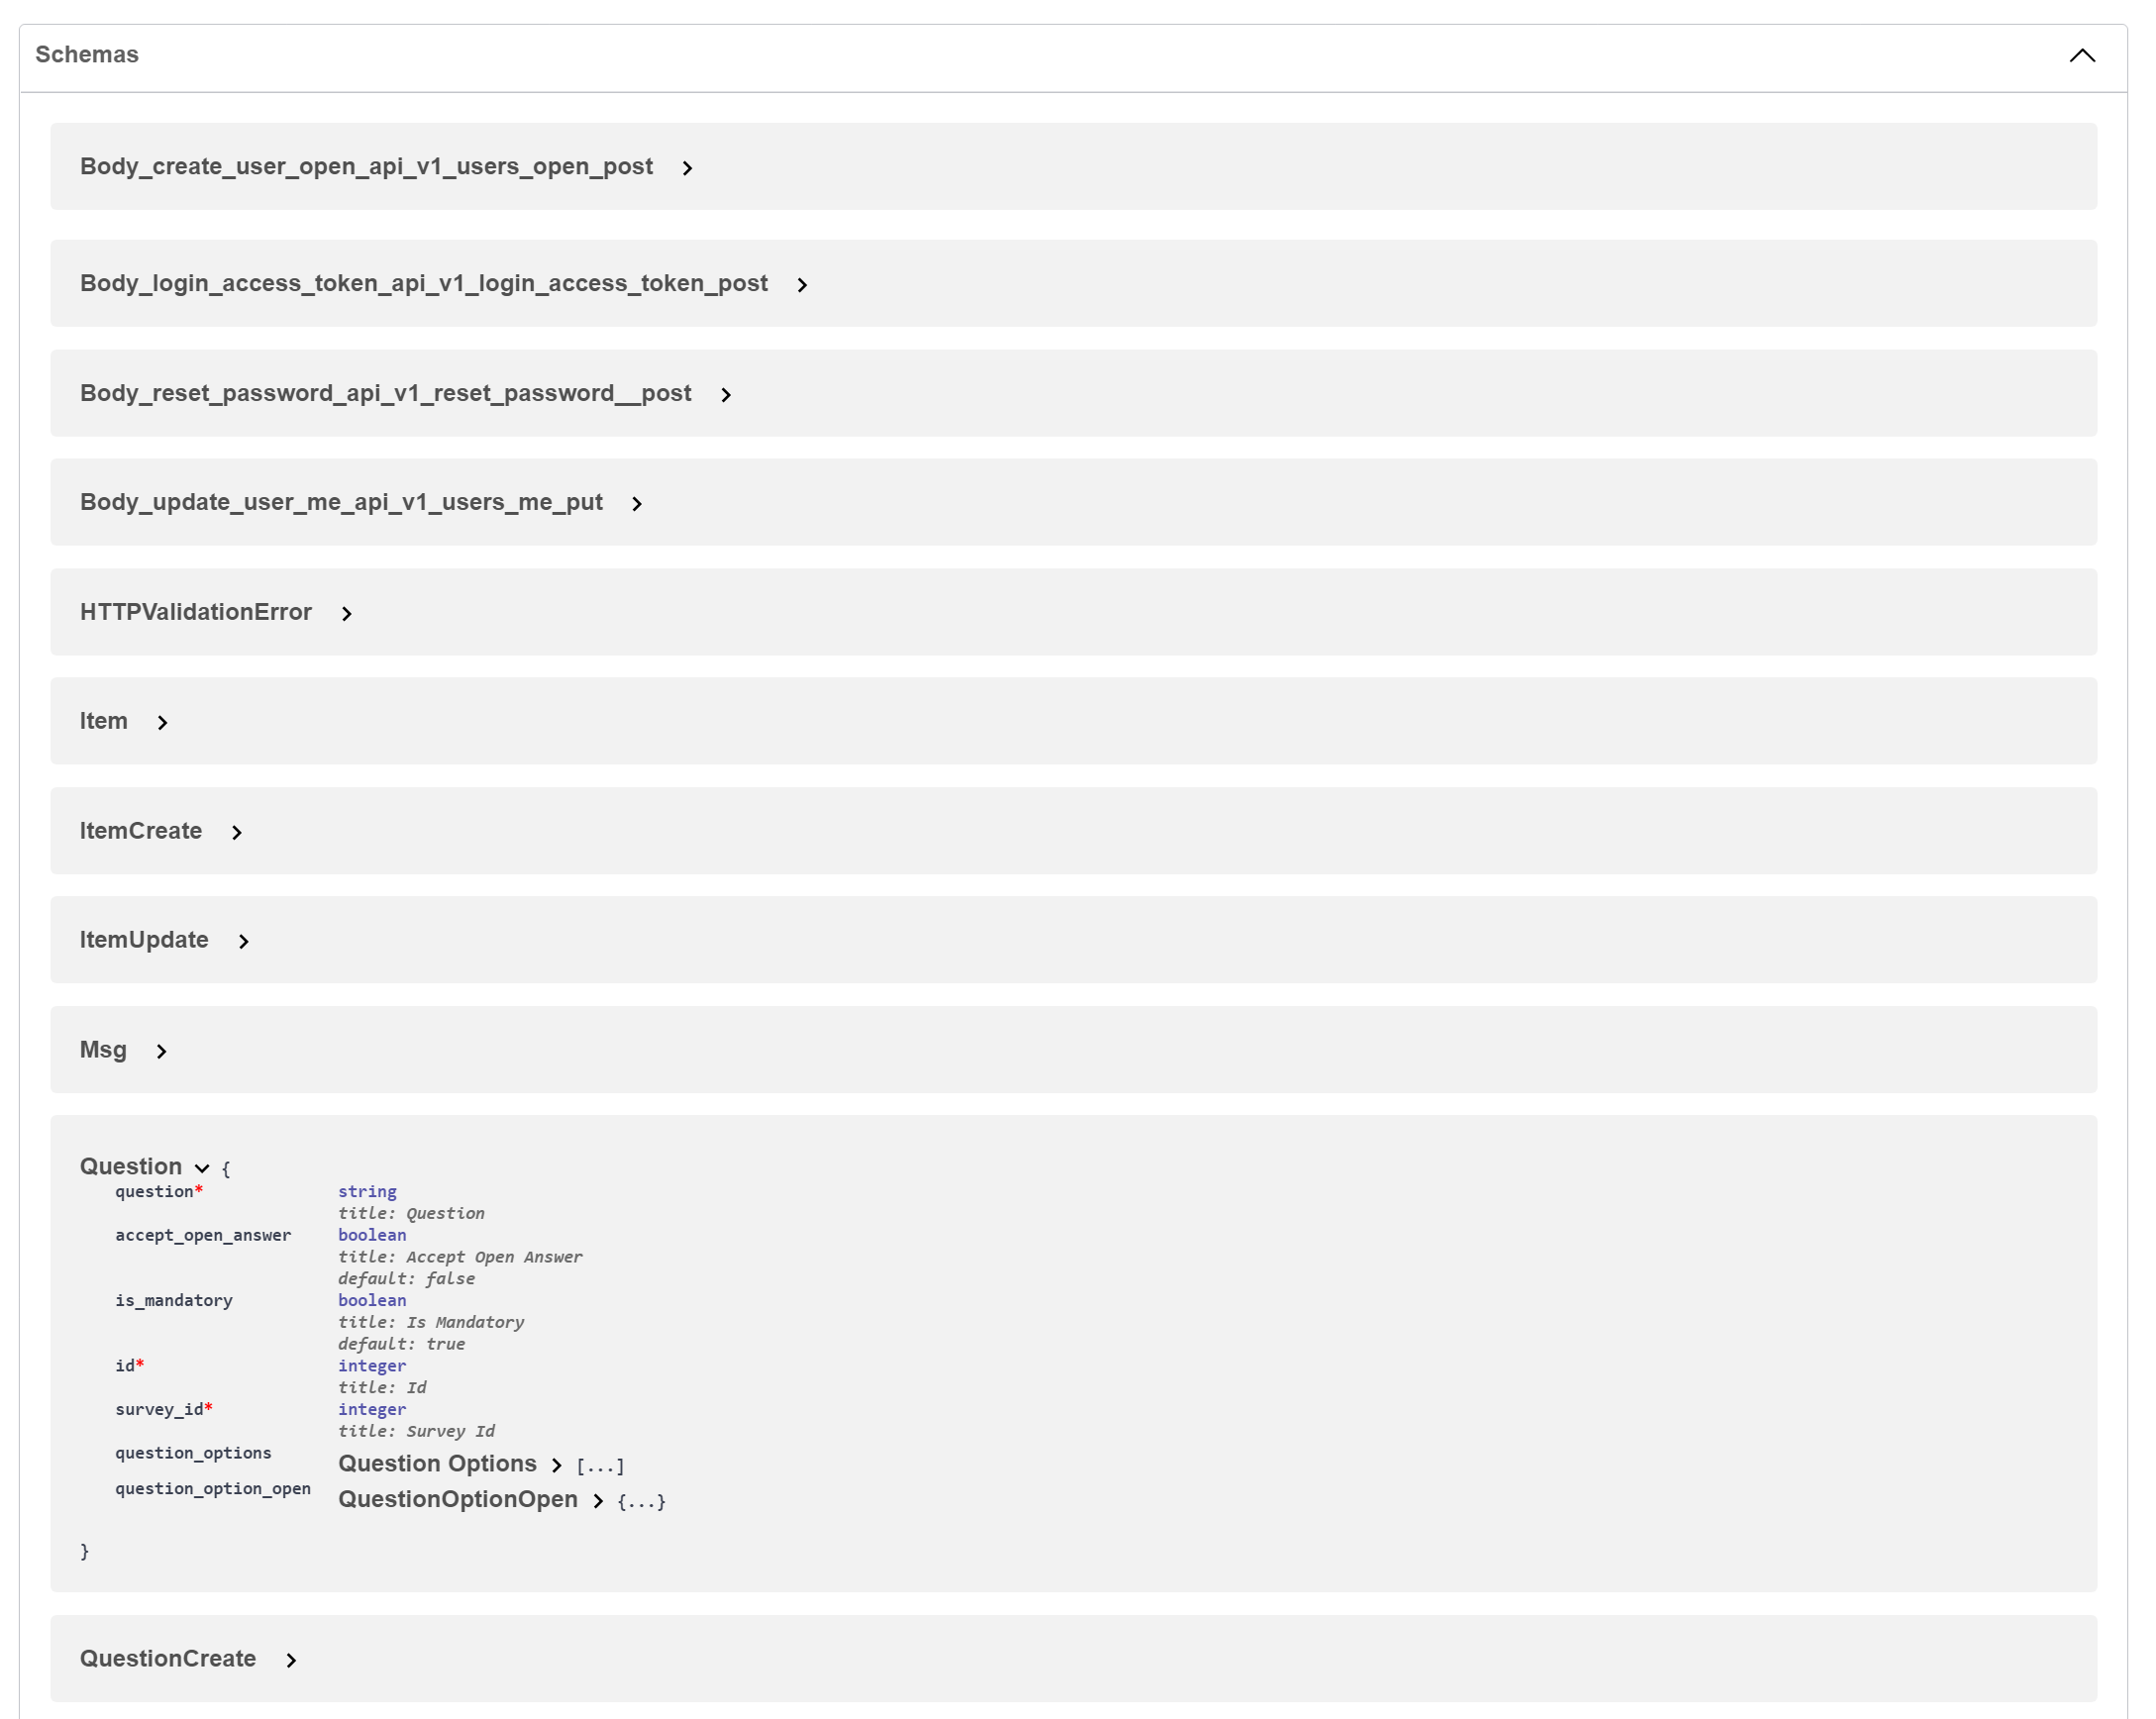
\includegraphics[scale=.20]{TT/img/implementacion/docs_6.png}
    \caption{Documentación 'docs' - Parte 6}
    \label{graphic:docs6}
\end{figure}

\subsubsection{Documentación de FastApi - 'redoc'}
Esta versión esta enfocada en la explicación sobre cada endpoint y los esquemas, en la figura \ref{graphic:redoc1} se puede apreciar la diferencia con la sección anterior. La interfaz de usuario se enfoca mas en informar al usuario la estructura de los endpoint y que datos requiere la API para realizar las peticiones que el usuario desea hacer.

\begin{figure}[!htb]
    \centering
    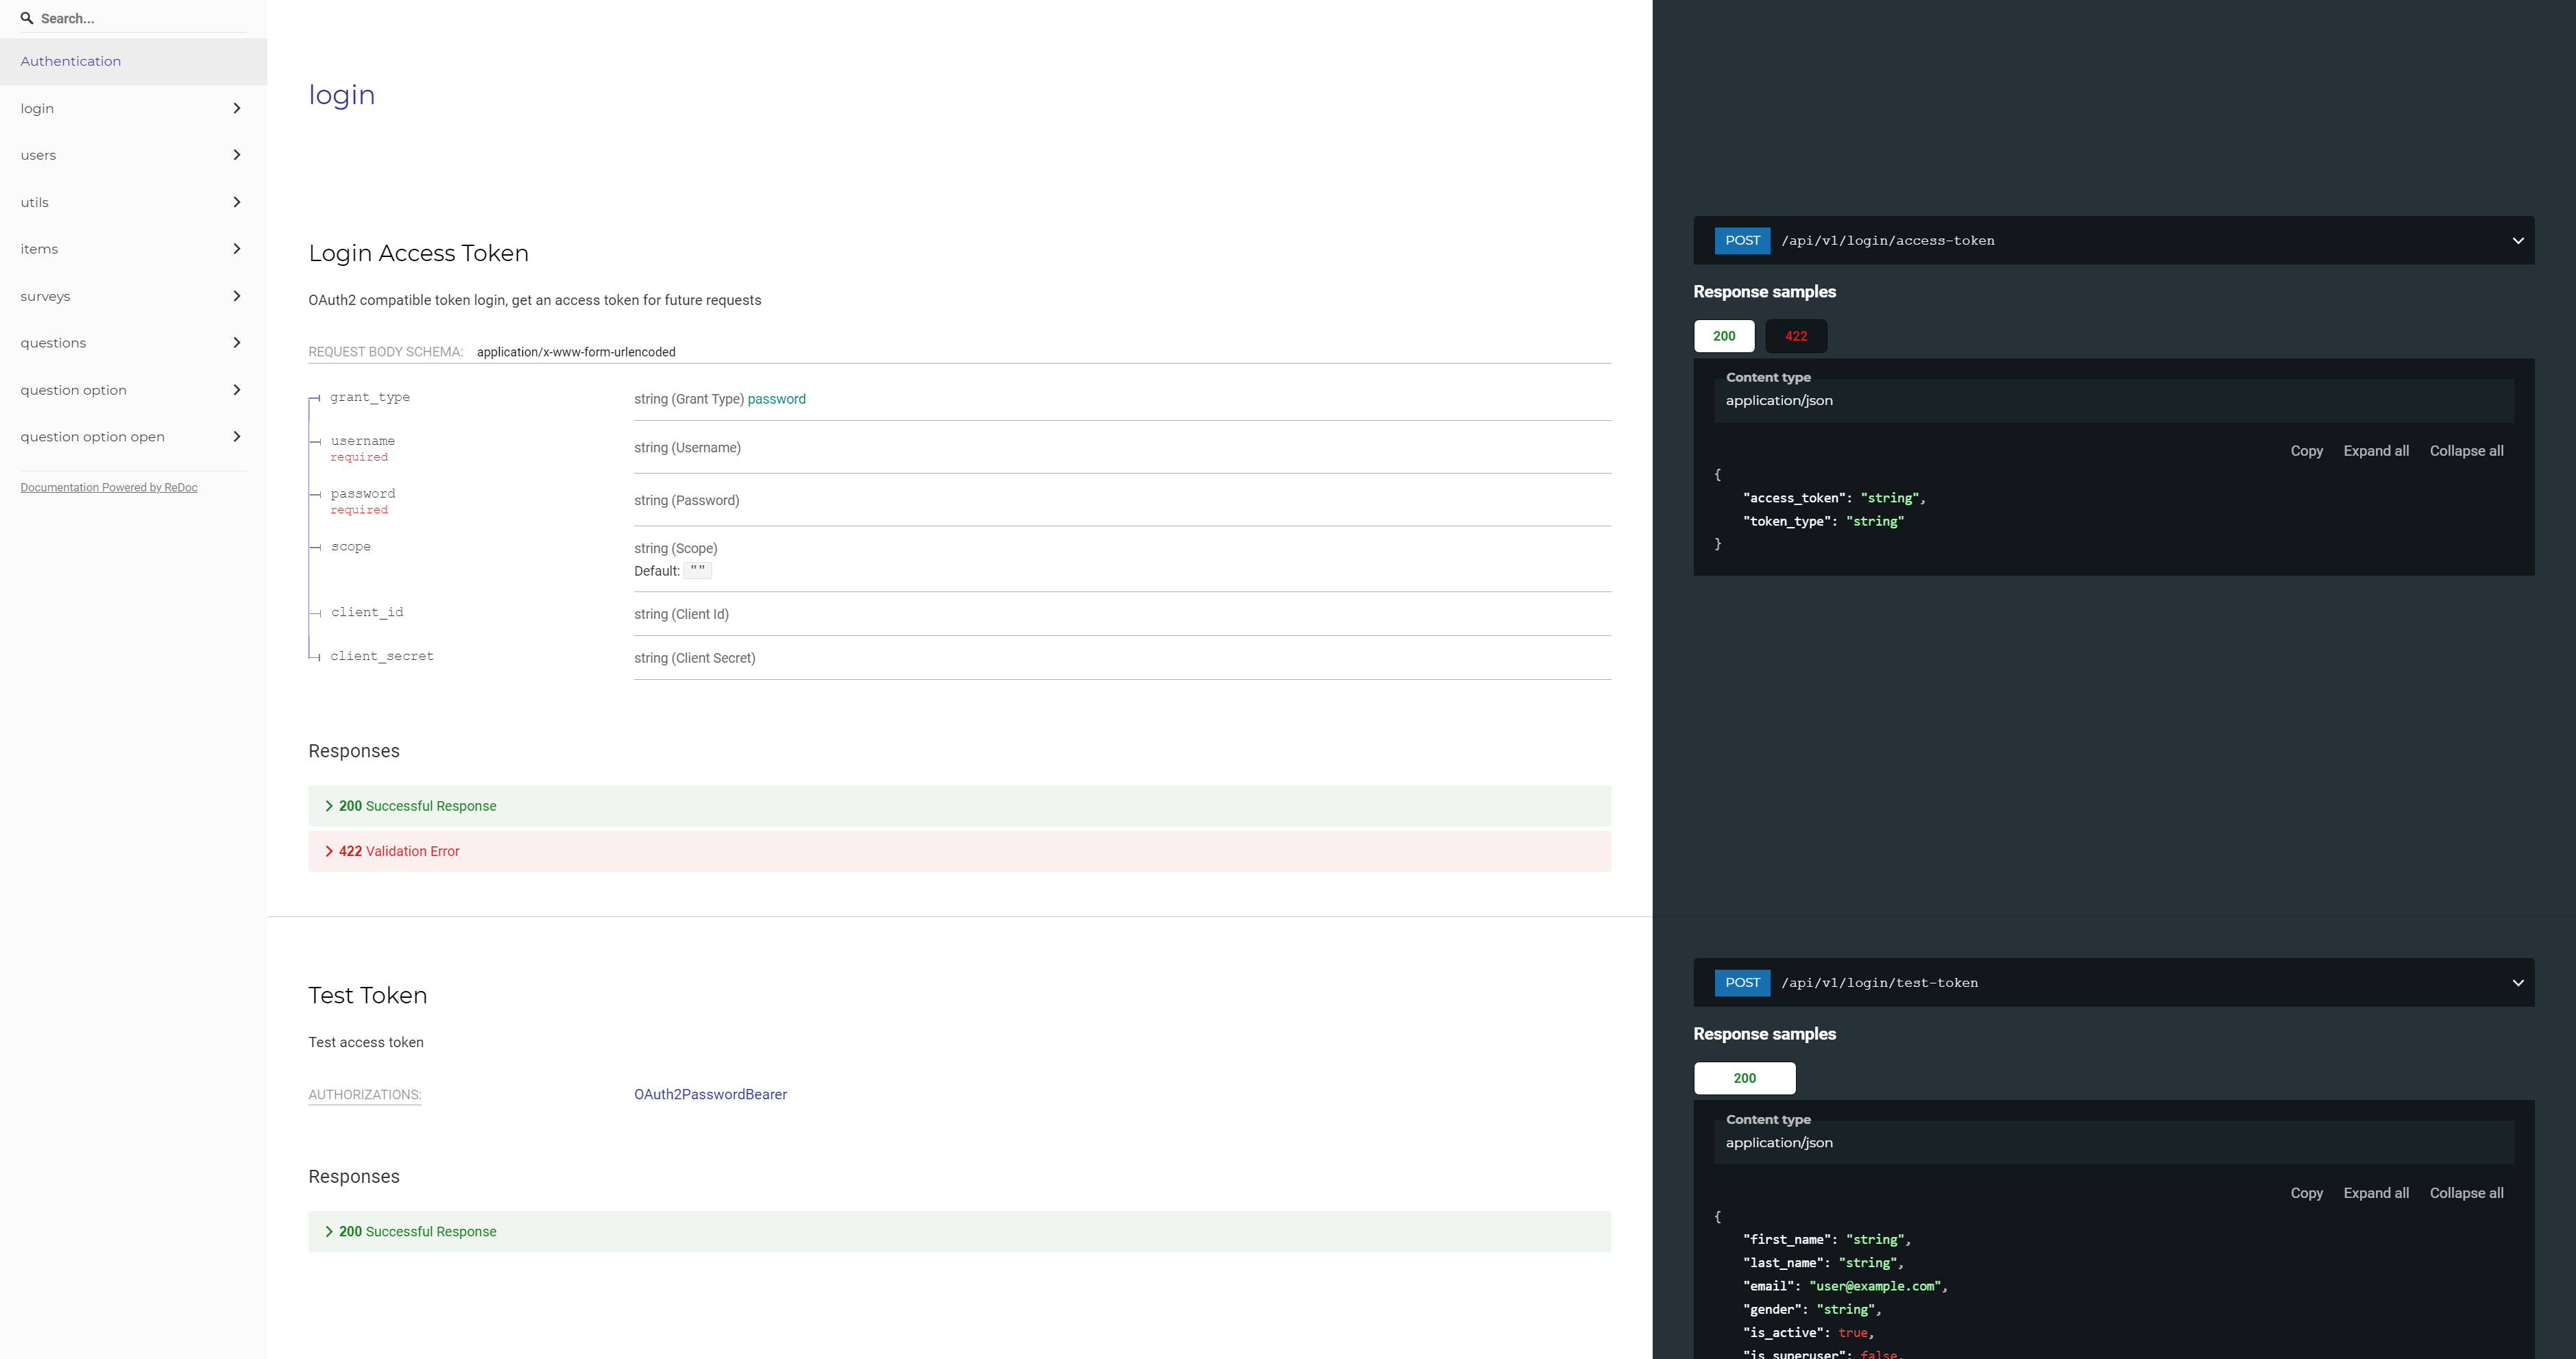
\includegraphics[scale=.25]{TT/img/implementacion/redoc_1.png}
    \caption{Documentación 'redoc' - Parte 1}
    \label{graphic:redoc1}
\end{figure}

En la imagen \ref{graphic:redoc2} se muestra la documentación del endpoint para crear usuario, del lado izquierdo estan listados los endpoint y al darle clic al que se desee, en este caso el endpoint de \textit{users} muestra las peticiones que se pueden hacer y el nombre de estas; en la parte central viene el nombre de la petición, describe el tipo de autorización que se requiere para poder usar el endpoint, describe como es el cuerpo el esquema de la petición los nombres de los campos y el tipo de dato que permite y al final viene detallada las respuestas.
\begin{figure}[!htb]
    \centering
    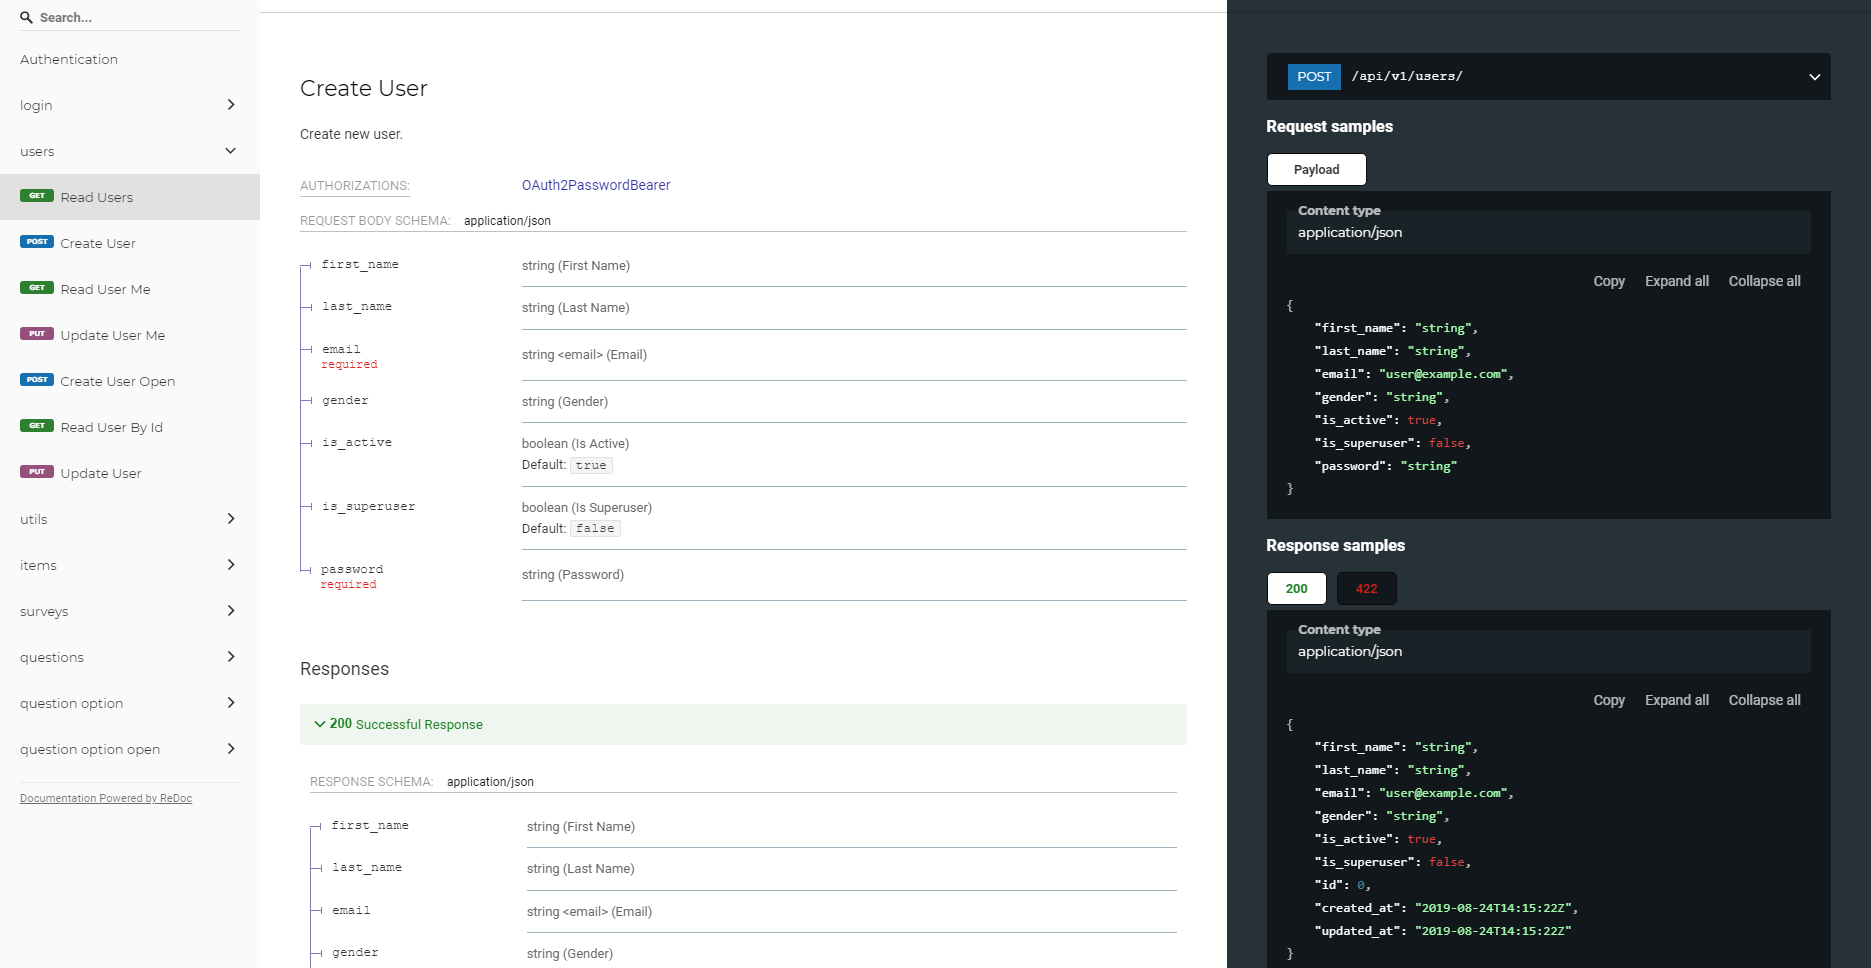
\includegraphics[scale=.25]{TT/img/implementacion/redoc_2.png}
    \caption{Documentación 'redoc' - Parte 2}
    \label{graphic:redoc2}
\end{figure}

Por último, en la imagen \ref{graphic:redoc3} y \ref{graphic:redoc4} se ve con mas detalle lo que se mostraba en las imágenes \ref{graphic:redoc1} y \ref{graphic:redoc2} del lado izquierdo, en esta sección detalla con mas precisión el endpoint, en la parte de arriba de las imágenes se muestra el tipo de petición y la URL de este mismo y al hacer clic de en el URL, nos desplegará el URL con el dominio en el que este configurado para su acceso mostrándose en la imagen \ref{graphic:redoc4}. En la parte central se muestra como se envían los datos, en todos los casos son 'aplication/json' junto con los campos y un ejemplo de como se deben de llenar para realizar la petición. Al final, se muestran los códigos de respuesta que ofrece la API, en la figura \ref{graphic:redoc3} se puede observar el código 200 que es cuando la petición se ha realizado exitosamente junto con la respuesta en formato json, por otro lado, en la figura \ref{graphic:redoc4} se detalla un error 422, este mensaje puede variar pero su estructura es la que se muestra ahí.

\begin{figure}[!htb]
    \centering
    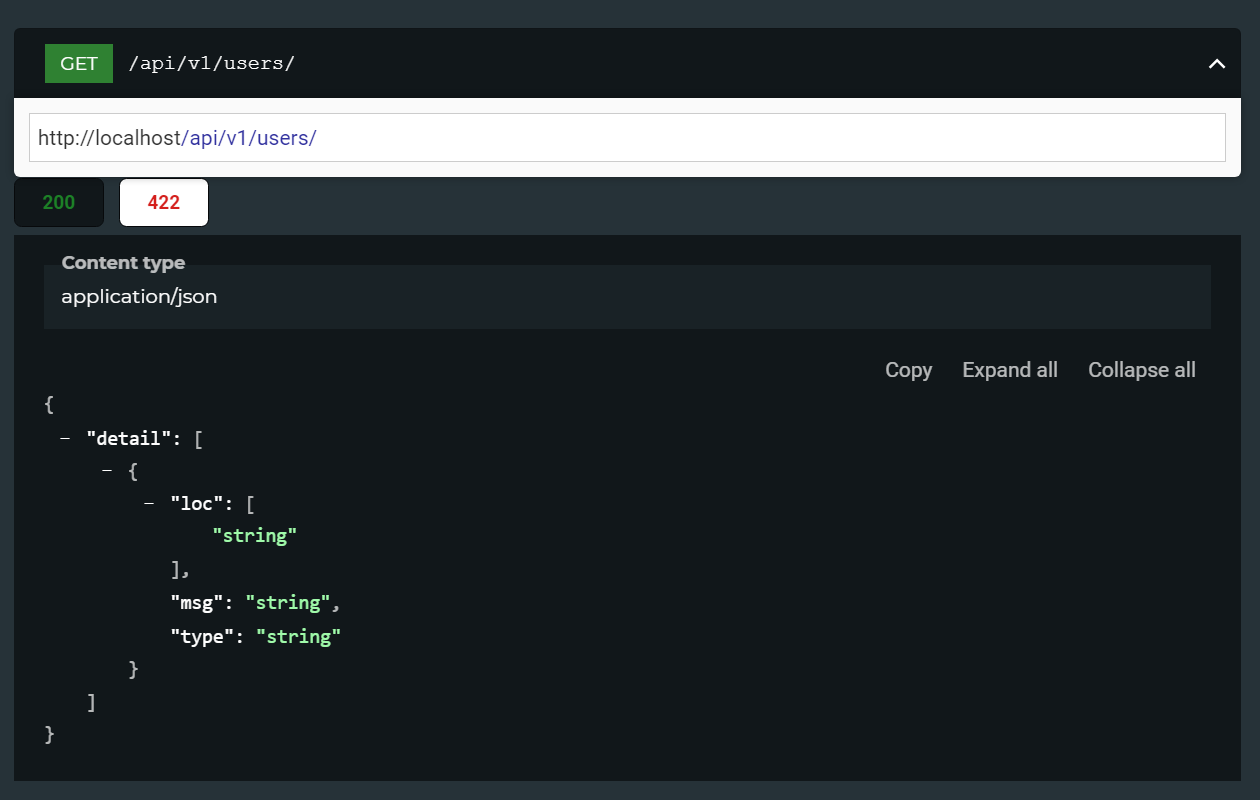
\includegraphics[scale=.40]{TT/img/implementacion/redoc_3.png}
    \caption{Documentación 'redoc' - Parte 3}
    \label{graphic:redoc3}
\end{figure}

\begin{figure}[!htb]
    \centering
    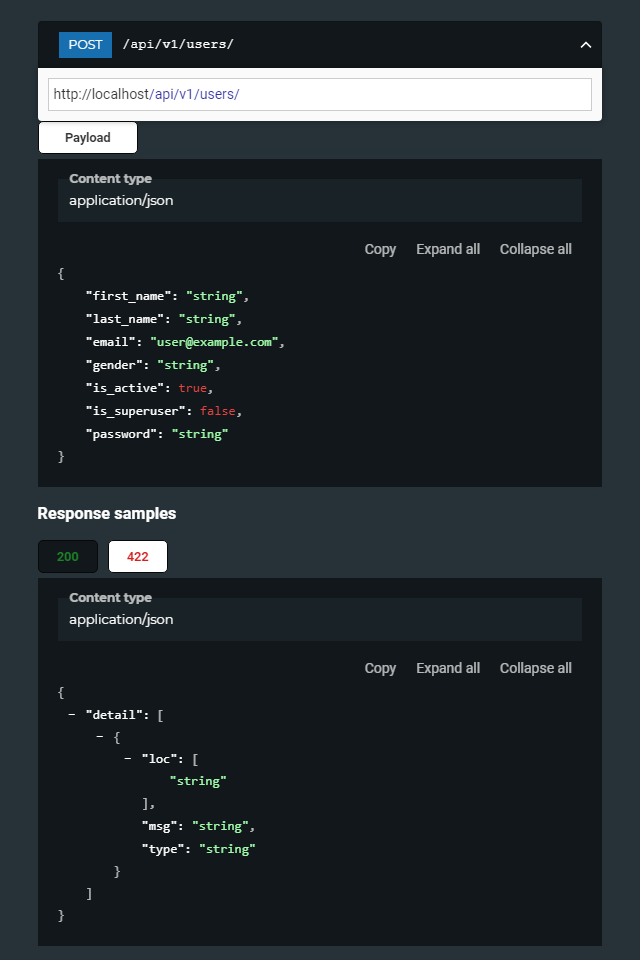
\includegraphics[scale=.40]{TT/img/implementacion/redoc_4.png}
    \caption{Documentación 'redoc' - Parte 4}
    \label{graphic:redoc4}
\end{figure}

\subsection{VueJS}
Para consumir la API usando una interfaz de usuario, se ha elegido usar el framework VueJS de JavaScript por su sencillez.
\subsubsection{Estructura del Frontend}
\subsubsection{Typescript}
\subsubsection{Interfaz de usuario}


\chapter{Conclusiones y Trabajo Futuro}
\epigraph{\textit{Good news, everyone!    
	}}{\textit{—  Professor Hubert J. Farnsworth}}
	\vspace*{8cm}
	\begin{center}
		\centering
		\includegraphics[width=10.5cm]{example-image}
	\end{center}
	\thispagestyle{empty}
	\newpage
\vspace*{2cm}

\section{Conclusiones}
  \blindtext[1]
 
\begin{comment}
\section{Trabajo Terminal II}
		\begin{itemize}
			\item
		\end{itemize}
\end{comment}
 

\subsection{Trabajo Futuro}
Los siguientes puntos son mejoras plausibles que podrían y deberían tomarse en cuenta para una versión futura del sistema.

\blindtext[1]
 


%Ver como se hicieron las otras ecuaciones
\listofmyequations
 \newpage
\appendix
\chapter*{Ejemplo de código} \label{aped.A}
\addcontentsline{toc}{chapter}{Ejemplo de código}
\section*{Ejemplo de programación en Flutter}
\addcontentsline{toc}{section}{Ejemplo de diseño en Flutter}
%\thispagestyle{empty}	
El siguiente diseño se encuentra en el ejemplo \ref{lst:diseño1}.
\newline

\begin{figure}[!ht]
    \centering
    
\includegraphics[scale = 0.9]{img/apendices/layaout.jpg}
    \caption{Diseño de ejemplo en Flutter}
    \label{fig:my_label}
\end{figure}


El diseño consiste en una estructura de árbol con un Container como widget raíz. El widget Container permite cierta personalización del widget hijo, en este caso algo de relleno alrededor del widget Row secundario. El widget Row describe una secuencia horizontal de widget: el primero es un Column (una secuencia vertical de widgets) de dos Text widgets, el segundo es un icono y el tercero es otro Text widget. Para que la segunda parte de la fila se vacíe a la derecha, el Column widget se envuelve en un entorno expandido, lo que permite que el Column ocupe todo el espacio horizontal disponible.
\newline
\begin{lstlisting}[language=Python, caption=Código de diseño de ejemplo, label={lst:diseño1}]
Widget titleSection = Container(
  padding: const EdgeInsets.all(32),
  child: Row(
    children: [
      Expanded(
        /*1*/
        child: Column(
          crossAxisAlignment: CrossAxisAlignment.start,
          children: [
            /*2*/
            Container(
              padding: const EdgeInsets.only(bottom: 8),
              child: Text(
                'Oeschinen Lake Campground',
                style: TextStyle(
                  fontWeight: FontWeight.bold,
                ),
              ),
            ),
            Text(
              'Kandersteg, Switzerland',
              style: TextStyle(
                color: Colors.grey[500],
              ),
            ),
          ],
        ),
      ),
      /*3*/
      Icon(
        Icons.star,
        color: Colors.red[500],
      ),
      Text('41'),
    ],
  ),
);

\end{lstlisting}

%\clearpage
%\appendix
%\includepdf[scale=0.85,pages=1,pagecommand=\chapter*{Patente de análisis de muestras}\label{Apend. B} \addcontentsline{toc}{chapter}{Patente de análisis de muestras}]{pdf/Glucometro-patenteUS7276147.pdf}
%\includepdf[pages=2-]{pdf/Glucometro-patenteUS7276147.pdf}

\clearpage
 % Aquí van las referencias
%BIBLIOGRAFÍA


  \linespread{1.5}
 

\nocite{*}
\bibliography{bib/bibliografia}

% Glosario
\printnoidxglossaries
\vspace*{5cm}
\begin{flushright}
	\textcolor{gray}{crafted with \heart\, using \LaTeX}
\end{flushright}
\end{document}